% $Id$
% $Log$
% To process this file:
% 
% (in tex directory), do the following with 
% codefile = ratecalc, readgeometry, random, classes, geometry, tallysetup,
% elementsetup, speciesetup, reactionsetup, materialsetup, pmisetup,
% problemsetup, outputbrowser:
%   gmake codefile.tex
%   pdflatex codefile.tex
%   mv codefile.pdf ../Doc
% update page numbers in href's to these files.
% rm degas2_all.html
% Remove old {theindex} from this file
% tth -e0 -Ldegas2_all < degas2_all.tex > degas2_all.html
% (this reads but does not update the degas2_all.aux file, so should
%  have that synched with the .tex file before running tth)
% In html file, replace ">Figure with .jpg">Figure
% pdflatex degas2_all.tex
% makeindex degas2_all
%
% Insert degas2_all.ind at end of this file. How about before TOC?
%
% pdflatex degas2_all.tex (will now have a hyperlinked index)
%
%  acroread -toPostScript degas2_all.pdf
%  (pdf2ps DOES NOT appear to work well)
%
%
\documentclass[12pt]{report}
% Macro for http reference inclusion, per hypertex:
\def\href#1#2{\special{html:<a href="#1">}{#2}\special{html:</a>}}
\makeindex
\usepackage{times}
% Use this line with pdflatex. The problem with this is that it
% doesn't use eps or ps formats with includegraphics. It
% will allow pdf or jpg.
% this is different from the usage with latex!
% Nonetheless, ``distill file.ps'' produces a pdf file that looks
% much better than a jpeg from xv.  Can use ``convert file.pdf file.jpg''
% (e.g., on tern) to nicely convert these pdf's to jpeg's.
%
\usepackage[pdftex]{hyperref}
\usepackage[pdftex]{graphicx}
% Do we need:
%
% \hyperbaseurl{http://w3.pppl.gov/degas2/Doc/} ??
%
% Use the following with latex, dvips -Pwww, and then distill:
% The problem with this is that the \tt titles choke distill.
% \usepackage[dvips]{hyperref}
% \usepackage{graphicx}
\begin{document}
% \input epsf
\title{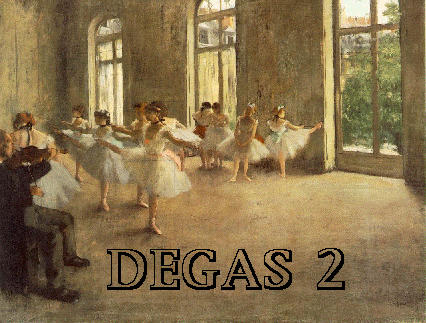
\includegraphics{degas2d}
User's Guide for DEGAS 2 \\
Edition 2.0\thanks{This file is written in \TeX. A hyper-linked PDF
file is generated from that source using {\tt pdflatex}. The ``2.0'' 
version number is a placeholder which will be superseded by the overall version
number of the code in the near future. Copyright \copyright 1999 PPPL.
Permission is granted to make and distribute verbatim copies of this manual
provided the copyright and permission notice is preserved on all copies.
Permission is granted to copy and distribute modified versions of this
manual under the conditions for verbatim copying, provided also that
the entire resulting derived work is distributed under the terms of a
permission notice identical to this one.
Permission is granted to copy and distribute translations of this manual
into another language, under the above conditions for modified versions.}}
\author{\vspace*{-0.5in} \\ Daren Stotler and Charles Karney \\ {\em Princeton Plasma Physics 
Laboratory} \\ Randall Kanzleiter \\ {\em Rensselaer Polytechnic Institute} \\
Jaishankar S. \\ {\em Institute for Plasma Research, India}}
\begin{abstract}
This is version 2.0 of the user's manual for DEGAS 2 - A
Monte Carlo code for the study of neutral atom and molecular transport 
in confined plasmas. It is intended to cover all aspects of DEGAS 2 from the
user's point-of-view: obtaining
the files, compiling them, setting up the input files, executing the
code,  and interpreting the output. 
References will be provided for the underlying physics, but the
essential aspects will be highlighted. Information for programmers
interested in modifying DEGAS 2 can be found within the source code
itself. Links to some of the more useful ones are provided.
\end{abstract}
\maketitle
\chapter{Introduction}

\section{Purpose of Monte Carlo Neutral Transport}
\index{Neutral Transport}
\index{Transport codes}
\index{Theory, transport}
\index{Boltzmann equation}

The interaction of neutral atoms and molecules with the background 
plasma is an important component in the physics of fusion research
plasmas. These
neutrals affect both the particle and energy balance  of the plasma,
providing a source of new plasma and a channel for heat transport across
the magnetic field that confines the charged particles. In addition, hot
neutrals which leave the plasma volume can interact with the wall of the
plasma chamber, sputtering impurities into the plasma and (in reactors)
possibly damaging the wall. Finally, these hot neutrals can also be used
for plasma diagnostics. Therefore, it is worth developing an accurate
description of the neutral behaviour.

The theory of neutral particle kinetics\cite{Tend87}
treats the transport of mass, momentum, and energy in a plasma due to
neutral particles that are themselves unaffected by magnetic
fields. This transport affects the global power and particle balances in
fusion devices, as well as profile control and plasma confinement
quality, particle and energy fluxes onto device components, performance
of pumping systems, and the design of diagnostics and the interpretation
of their measurements.  Though analytic models (solving the
Boltzmann equation for the neutrals or using the diffusion approximation),
both single- and multi-species, have been used to study neutral transport,
a variety of approximations must be made. Some numerical methods for solving
the Boltzmann equation use simplified geometries and atomic physics. On
the other hand, the Monte Carlo approach to integrating the Boltzmann
equation can treat in great detail asymmetric geometries and complex
atomic physics and wall interactions. Because of the similarity in the
problems, Monte Carlo neutral transport codes can build on the techniques
developed for neutron transport in reactor design\cite{Span69}.

\section{Need for DEGAS 2}
\index{DEGAS}

The predecessor to DEGAS 2 was  DEGAS\cite{Heif82}, a widely used and well
documented code. However, two events pointed out its limitations.
\begin{itemize}
\item The combined DEGAS-B2 code was too slow 
(about 100 Cray hours)\cite{Stot92}. 
The stronger the coupling between neutral and plasma species, the more 
difficult it is to arrive at a converged solution. In this case which 
looked at a high recycling
divertor for a compact, high field reactor, hundreds or thousands of complete
Monte Carlo profiles must be carried out in order to couple effectively
to a fluid code. 
\item The problem physics was difficult to modify. In the radiative and 
detached divertor
regimes being investigated for future reactors, it is believed that the list
of important atomic processes will grow to include elastic collisions and
molecular hydrogenic species other than ground state H$_{2}$.
\end{itemize}

Hence, it was decided that a new code should be written which draws
on the extensive experience at PPPL and that from Garching and
J\"{u}lich.
The philosophy behind DEGAS 2 was defined during 1992-1993:
\begin{itemize}
\item  High speed, 
\item  Flexibility,
\item  Ease-of-use,
\item  Well documented.
\end{itemize}


\section{DEGAS 2 Features}
\index{Object oriented programming}
\index{Allocation, memory}
\index{Macros}
\index{FWEB}

An effort was made to realise the above mentioned objectives of
DEGAS 2 by the following means:
\begin{itemize}
\item Improve speed relative to DEGAS by utilizing the 
``track length'' estimator.
\item Ensure flexibility by designing the code using quasi-object oriented
programming techniques. The modifier ``quasi'' refers to the fact that DEGAS 2
is written in FORTRAN (compatible with FORTRAN 77 and FORTRAN 90). Even though
the basic ``classes'' in the problem have been abstracted, the degree of
encapsulation actually achieved (via pre-processor macros) in DEGAS 2 is 
limited. Furthermore, there is no provision for inheritance within this
programming environment.
\item Provide an easy-to-use and well documented code by writing it with the
FWEB\cite{FWEB} package. FWEB provides the powerful preprocessing and
macro facility which underlies the ``quasi-object oriented''  implementation
and internal \TeX\ documentation.
\end{itemize}

\index{NetCDF}
\index{HDF}
\index{CVS}
\index{Processing, parallel}
Other significant features of DEGAS 2 include:
\begin{itemize}
\item Dynamic memory allocation for optimal performance in large problems,
\item Operation on a number of UNIX platforms,
\item Input and output data stored in self-describing, platform-independent 
binary files.
Presently, the main code uses exclusively
netCDF\cite{nCDF} (Network Common Data
Format) files for input and output. However, a simple post-processing
utility is included which generates graphics and data in  
HDF\cite{HDF} (Hierarchial Data Format) files. 
Hopefully, a single format will be settled upon eventually.
\item Parallel execution on distributed workstations and massively
parallel computers. This is the most promising
technique for improving the speed of DEGAS 2.  The reason is that most of
the future advancements in computer speed will result from increases in the
number of processors. Parallel processing is practical to Monte Carlo since
the amount of communication required per computation is small.
\item High quality coding standards.
Good programming practices such as use of the {\tt implicit none} statement
and an assertion facility help to ensure that the code works properly. 
This document will eventually describe a basic test suite which actually
demonstrates that the code is correct. In the code design process, clarity
has been given a high priority as well, facilitating readability and
maintainability.
\item Code versions numbered and documented with the ``CVS'' (concurrent
version system) package.
\end{itemize}

\chapter{Background}

\section{Generic Monte Carlo Algorithms}
\index{Monte Carlo}
\index{Tracking}
\index{Random}
\index{Scoring}
\index{Distribution, probability}
\index{Generators, random number}

Monte Carlo methods generally involve sampling from some ``parent population''.
The sampling process is usually facilitated by pseudo-random numbers generated
via a numerical algorithm. The quantity or quantities sampled are then 
used as input to a subsequent (deterministic) calculation which results in the
desired output. This process is repeated a number of times, so as to 
thoroughly sample the parent population, and a distribution of the output
data is compiled. In some cases, only the mean of this distribution is of 
interest (as well as some estimate of its error), while in other cases, the
distribution itself is the objective.

Note that the process being simulated need not be random. For example, Monte
Carlo techniques may be the only way of computing the volume of some complex
three-dimensional object. This is just one example of the versatility of
Monte Carlo techniques. But, Monte Carlo is not always the most efficient
solution for a problem because of the significant computational
effort required. Two reasons for using Monte Carlo are: 
\begin{enumerate}
\item No other solution is available.
\item The details of the problem are sufficiently important that no 
approximations
can be tolerated.
\end{enumerate}

In the case of particle transport, the latter reason is usually invoked.
Examples of Monte Carlo particle transport include:
\begin{enumerate}
\item Neutron tranport in fission devices,
\item Radiation transport,
\item Electron transport in semiconductors,
\item Neutral particle transport in plasmas.
\end{enumerate}

\subsection{Sampling a Distribution}

The most fundamental process of a Monte Carlo simulation is the sampling
of probability distributions. Typical examples for a particle simulations
would be:
\begin{enumerate}
\item Choosing a velocity vector from a Maxwellian distribution,
\item Picking a particle from a spatially varying source,
\item Determining the distance to the next collision.
\end{enumerate}

\subsection{Sampling Distance to Next Collision}
\label{SamplingDistance}

To illustrate the third case, consider particles with a total, 
macroscopic cross
section $\Sigma_{t}$. We write the  {\em probability density function} 
for having 
the next collision between $x$ and $x + dx$, $p(x)  \: dx$, as:
\begin{equation}
p(x) dx = \Sigma_{t} \exp(-\Sigma_{t} x)   \: dx.
\end{equation}
Then, the  {\em cumulative probability distribution} $P(y)$,
\begin{equation}
P(y) = \int_{0}^{y} p(x)  \: dx, 
\end{equation}
is the probability of having a collision for any $x \leq y$. Note that
$P(0) = 0$ and $P(\infty) = 1$.

\begin{figure}
% \epsfverbosetrue
\begin{center}
\leavevmode
% \epsfxsize=3in
% \epsfbox{MC_Sampling2.eps}
% 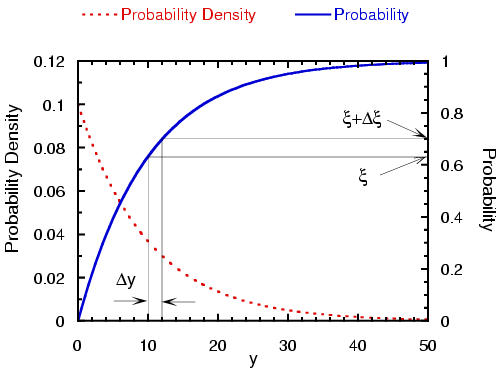
\includegraphics[width=3in]{MC_Sampling2.eps}
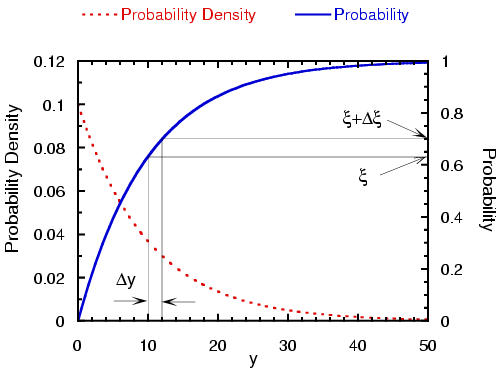
\includegraphics[width=4in]{MC_Sampling2}
\caption{A uniformly sampled $\xi$ value is translated into a sample of $y$
distributed according to the ``Probability Density'' curve using the integrated
``Probability'' curve.}
\label{MCSampling}
\end{center}
\end{figure}

As suggested by the above figure, $P(y)$ can be sampled by choosing a 
uniformly distributed random number $\xi$, with $0 \leq \xi < 1$. For
this example, $P(y)$ is easily computed and inverted so that
\begin{equation}
 y = - \frac{\ln \xi}{\Sigma_{t}},
\end{equation}
where we have surreptitiously replaced $1 - \xi$ with $\xi$ since both
are uniform over the unit interval. Again the logic of this process,
as depicted in the figure, is that if $\xi$ is
uniformly distributed, then numbers between $\xi$ to $\xi + \Delta \xi$ 
are chosen with the same frequency as particles having collisions between
$y$ and $y + \Delta y$. Thus, $y$ is the sampled
  {\em distance to next collision}.

\subsection{Sampling More Complicated Distributions}

Because of the simplicity of the functional form of the collision probability
density function, the distance to the next collision can be easily sampled
using a single, uniform random number. If this were not the case, more
general methods, such as this \emph{rejection technique}, would have 
to be employed.

As an example, consider the sampling of a velocity $v$ from a Maxwellian 
distribution,
\begin{equation}
p(v) = \frac{1}{\sqrt{\pi} v_{\rm th}} \exp \left[ - \frac{(v -
v_{0})^{2}}{v_{\rm th}^{2}} \right].
\end{equation}
For simplicity, limit the $v$ values to $|v - v_{0}| < M v_{\rm th}$ for some
appropriate $M$.

\begin{figure}
% \epsfverbosetrue
\begin{center}
\leavevmode
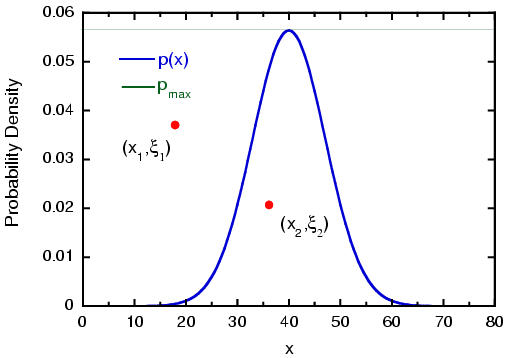
\includegraphics[width=4in]{MC_Rejection2}
\caption{Values of $x$ distributed according to $p(x)$ can be sampled by
uniformly selecting $(x,\xi)$ pairs and tossing out ones with $\xi > p(x)$.}
\label{MCRejection}
\end{center}
\end{figure}

Now, we choose a pair of random numbers $(x, \xi)$ with $x$ uniformly 
distributed over the interval
$v_{0} - M v_{\rm th} \leq x < v_{0} + M v_{\rm th}$ and $\xi$ uniform over 
$0 \leq \xi < p_{\rm max}$, where $p_{\rm max}$ is the maximum value of $p(v)$.
If $\xi < p(x)$, accept this $x$ as the sampled velocity. Otherwise, if 
$\xi > p(x)$, reject these $(x, \xi)$ and sample another pair. That the
resulting set of $x$ values is distributed as required can be seen by studying
the figure above. This figure also makes the case that the rejection approach
may not be very efficient for sampling a Maxwellian (indeed, DEGAS 2 
uses the well-known Box-Mueller method for this task).

In general, a rejection technique factors the probability density $p(x)$ into 
two functions, $p(x) = g(x) h(x)$, where it is known how to sample $x$ from
the function $g(x)$. The acceptance condition is just $\xi < h(x)$. The
Maxwellian example simply sets $g(x) = 1$.

\section{Particle Transport}

One of the main benefits of doing Monte Carlo particle transport is that 
most of the time the algorithm can be understood directly from a physical
picture. Namely, we think of the code as tracking particles through a
medium and having collisions with probabilities determined from the cross
sections of the various collision processes. The outcome of those collisions
is the same as for the actual physical particles, and so on. This is 
known as the \emph{analog} description of Monte Carlo particle transport.

In this section, we want to give a rough idea of how this picture relates
to the integral equations which provide the actual mathematical basis
for Monte Carlo techniques. Only from these equations can we understand
the {\em non-analog} techniques (the rejection technique described in
the previous subsection is a non-analog technique) used to make the Monte 
Carlo process more efficient. We hope to familiarize the reader with
the integral equations to the point where more detailed 
references\cite{Span69,Reit92} can be readily digested.

From an analog point-of-view, we imagine a Monte Carlo particle simulation
as consisting of four parts:
\begin{enumerate}
\item A way to sample an initial particle distribution,
\item A way to treat particles from one point in space to another,
\item Tools to treat ``interesting things'' that might happen along the way,
\item Some useful quantities to compute and record at each stage of the 
process.
\end{enumerate}
The last of these, referring to ``scores'' and their ``estimators'' will
be addressed in Sec.~\ref{Estimators}.

\subsection{Motivating the Integral Equation}

The initial particle distribution, or source, is given by a probability 
density function $Q(x) > 0$. We take $x$ here to represent a point in 
phase space so that this function provides both the velocity and spatial
distribution of the source. 

The tracking of particles is described in the integral equation by a function
$L(y \rightarrow x)$ which gives the probability that a particle starting 
at a point $y$
in phase space ends up at point $x$. This function includes the ``interesting
things'' (collisions) 
that might happen along the way, as we will describe in the next 
subsection.

Using these two functions, we can write the {\em density of particles
arriving at $x$}, $\chi(x)$ as the sum of two pieces:
\begin{enumerate}
  \item Arrivals directly from source: $Q(x)$.
  \item Particles transported from elsewhere: 
\begin{equation}
\int \chi(y) L(y \rightarrow x)  \: dy
\end{equation}
   \end{enumerate}
And we have
\begin{equation}
\chi(x) = Q(x) + \int \chi(y) L(y \rightarrow x)  \: dy.
\end{equation}

\subsection{Transport and Collision Kernels}

In order to describe the kernel $L(y \rightarrow x)$ in more detail, substitute
for $y$ and $x$ the phase space variables $(\vec{r},\vec{v})$ and a species
index $i$. The kernel $L$ can then be broken into two pieces:
\begin{equation}
L(\vec{r}^{\prime}, \vec{v}^{\prime}, i^{\prime} \rightarrow \vec{r}, 
\vec{v}, i) = T(\vec{r}^{\prime} \rightarrow \vec{r}; \vec{v}, i) C(\vec{v}^{\prime}, 
i^{\prime} \rightarrow \vec{v}, i; \vec{r}),
\end{equation}
where $T(\vec{r}^{\prime} \rightarrow \vec{r}; \vec{v}, i)$ 
is the (probability) density of particles leaving a 
collision at $\vec{r}^{\prime}$ and having a subsequent collision at $\vec{r}$. 
The ``;'' is used in
the arguments of $T$ and $C$ to separate changing parameters (on the left) from
those held fixed (on the right). Basically, sampling from $T$ is as 
described in
Section~\ref{SamplingDistance}.

Collisions are described by $C(\vec{v}^{\prime}, i^{\prime} \rightarrow 
\vec{v}, i; \vec{r})$ which provides the probability
that a particle of velocity $\vec{v}^{\prime}$, species $i^{\prime}$ 
will have a collision resulting in 
a particle of velocity $\vec{v}$, species $i$. In practice, $C$ is a 
sum over the physical
reactions in which species $i^{\prime}$ participates.

\subsection{Integral Equation Details}
\label{IntegralEquationDetails}

One of the problems with reading Monte Carlo particle references is that
there are several slightly different ``quantities of interest'' equivalent
to $\chi(x)$. Furthermore, there is no well-established notation for those
quantities. In this subsection, we attempt to list these various quantities
and to provide a detailed form of an integral equation for later reference.

The quantity $\chi(x)$ is called the {\em post-collision density}. The 
origin of this designation should be clear from the previous discussion.
Equivalently, the integral equation can be written in terms of the 
{\em pre-collision density} $\psi(x)$. The two are related by
\begin{equation}
\psi(\vec{r},\vec{v},i) = \int d^{3}r^{\prime} 
\chi(\vec{r}^{\prime},\vec{v},i) 
T(\vec{r}^{\prime} \rightarrow \vec{r}; \vec{v},i).
\label{post2pre}
\end{equation}

It is this pre-collision density which is most closely related to the 
more familiar particle flux $\Phi$ and particle
distribution function $f$ by the definitions:
\begin{equation}
\psi(\vec{r},\vec{v},i) = \Sigma_{t}(\vec{r},\vec{v},i) \Phi(\vec{r},\vec{v},i)
 = \Sigma_{t}(\vec{r},\vec{v},i) |\vec{v}| f(\vec{r},\vec{v},i).
\end{equation}

The integral equation for $\psi$ bears a strong resemblance to that for
$\chi$. We write it out here in detail to illustrate the details as well as 
to provide a reference point for the rest of the document and other
reading:
\begin{eqnarray}
\psi(\vec{r},\vec{v},i) & = & S(\vec{r},\vec{v},i) \nonumber \\
& & \quad + \int_{0}^{\infty} dR \:
\int d^{3}v \: 
C(\vec{v^{\prime}},i^{\prime} \rightarrow \vec{v},i; \vec{r} - \vec{\Omega} R) 
\nonumber \\
& & \qquad \quad \times T(\vec{r} - \vec{\Omega} R \rightarrow \vec{r}; \vec{v},i)
\psi(\vec{r} - \vec{\Omega} R, \vec{v^{\prime}},i^{\prime}),
\end{eqnarray}
where
\begin{equation}
S(\vec{r},\vec{v},i) = \int_{0}^{\infty} dR \: 
Q(\vec{r} - \vec{\Omega} R, \vec{v}, i)
T(\vec{r} - \vec{\Omega} R \rightarrow \vec{r}; \vec{v},i),
\end{equation}
and
\begin{equation}
T(\vec{r} - \vec{\Omega} R \rightarrow \vec{r}; \vec{v},i)
= \Sigma_{t}(\vec{r},\vec{v},i) \exp \left[ - \int_{0}^{R} dR^{\prime} \:
\Sigma_{t}(\vec{r} - \vec{\Omega} R^{\prime},\vec{v},i) \right].
\end{equation}
The actual form of the collision kernel $C$ need not be written down
here. Instead, in this document we'll only talk about it's implementation
from an analog point of view. The only additional piece of information
about it that we could add to the above equations is that $C$ consists
of a sum over the relevant collision processes involving species $i^{\prime}$.

The approach of writing the path integrals as above instead of as general
phase-space volume integrals with the path enforced via 
delta-functions\cite{Reit92}
was copied from Case and Zweifel\cite{Case67}
We find that this leads to expressions which are easier to work
with and think about.

\section{Estimators}
\label{Estimators}

The objective of the Monte Carlo calculation is to evaluate integrals over the
distribution function:
\begin{equation}
I(g) \equiv \int d^{3}r d^{3}v f(\vec{r},\vec{v})
g(\vec{r},\vec{v}).
\end{equation}
For example, if we wish to estimate a reaction rate 
$\rho \equiv \Sigma |\vec{v}|$,
\begin{equation}
I(\rho) = \int d^{3}r d^{3}v \Sigma \Phi(\vec{r},\vec{v}).
\end{equation}

Values of $\rho$ are accumulated along the random walk of the neutral flight
and used to estimate $I(\rho)$. The mathematical description of this
accumulation process is called the {\em estimator} of $I$. 

\subsection{Simple Estimators}
\label{SimpleEstimators}

Consider a random walk $\gamma$ which consists of $k$ steps,
$(x_{1}, x_{2}, \ldots, x_{k})$. I.e., the
particle is absorbed or otherwise terminated at the $k$th step.
The simplest estimator involves writing down the value of $\rho$
at the point of absorption. Thus, the absorption estimator is
\begin{equation}
\xi_{a}(\gamma) = \frac{\rho}{\rho_{a}} w \chi_{V},
\end{equation}
where $\rho_{a}$ is the absorption rate in the volume of interest
$V$ and $w$ is the statistical weight of the particle (constant for
this random walk process). The function $\chi_{V}$
\begin{equation}
\chi_{V} (x_{m}) = \left \{ \begin{array}{ll}
                        1 & \mbox{if $x_{m} \in V$} \\
                        0 & \mbox{if $x_{m} \not\in V$}
                       \end{array}
                         \right.,
\end{equation}
just permits the score to be localized to the volume of interest.

The expectation value of the estimator is just the sum over all
possible random walks $\gamma$ of the probability of each
walk $P(\gamma)$ times the corresponding estimator,
\begin{equation}
E(\xi_{a}) = \sum_{\gamma} P(\gamma) \xi_{a}(\gamma).
\end{equation}
Obviously, only one data point is collected for each random walk.

We can instead accumulate a score at each step (scattering collision)
of the random walk.
\begin{equation}
\xi_{c1}(\gamma) = \sum_{m=1}^{k} \left[ 
\frac{ \rho_{a} (x_{m}) }{ \rho_{t} (x_{m}) } \right] w
\chi_{V} (x_{m}), 
\end{equation}
where $\rho_{t} = \rho_{a} + \rho_{s}$ is the total reaction
rate for the particle, with $\rho_{s}$ being the scattering
rate. The subscript $c1$ denotes the first collision estimator
described here. The expectation value of the estimator is again
formally written as
\begin{equation}
E(\xi_{c1}) = \sum_{\gamma} P(\gamma) \xi_{c1}(\gamma).
\end{equation}
Because of the greater amount of data accumulated along each particle
track, the variance of this estimator will usually be smaller
than that of the absorption estimator.

Consider now a random walk process in which absorption is forbidden.
This is our first departure from the usual analog processes.
Instead of an absorption, the weight of the particle is reduced
at each scattering collision by its survival probability.
So, at the $m$th step of the walk the weight of the particle is
\begin{equation}
w_{m} = w  \prod_{j=1}^{m} \frac{ \rho_{s} (x_{j}) }{ \rho_{t} (x_{j}) }.
\end{equation}
The flight must be terminated in some manner; the usual practice
is to have it undergo Russian roulette\cite{Span69} when 
$w_{m} < w_{\rm min}$, where $w_{\rm min}$ is some specified 
minimum weight. The collision estimator for this nonanalog
random walk process is then
\begin{equation}
\xi_{c2}(\gamma) = \sum_{m=1}^{k} w_{m} \left[ 
\frac{ \rho_{a} (x_{m}) }{ \rho_{t} (x_{m}) } \right]
\chi_{V} (x_{m}).
\label{nonanalog}
\end{equation}

For formal proofs that these expectation values do indeed yield $I(\rho)$,
see Spanier and Gelbard\cite{Span69}.

\subsection{Generalized Collision and Tracklength Estimators}

Two principal
estimators are used in DEGAS 2. One is a generalization of the 
collision estimator described in the previous subsection; the other
is the tracklength estimator.

These estimators can be obtained by making a slight modification of the
derivation given by Macmillan\cite{Macm67} (who had improved upon an
earlier approach described by Spanier\cite{Span66}). To make the connection
to DEGAS 2 clearer, we replace the $\Sigma$ and $d$ variables of Macmillan
with $\rho$ and $t$.

Macmillan's paper, like the earlier one by Spanier, aims to derive the 
tracklength estimator. Collisions are described as either
scatterings, rate $\rho_{s}$, or absorptions $\rho_{a}$. The 
starting point is the nonanalog random walk process described in
Sec.~\ref{SimpleEstimators}. The probability of an event occurring in
a time interval $dt$ is $(\rho_{s} + \rho_{a}) \, dt$. Again, the weight
reduction factor applied at each scattering 
is $\rho_{s} / (\rho_{s} + \rho_{a})$.

The trick used by Spanier is to introduce a fictitious ``delta scattering''
that has no impact on the particle's trajectory or weight. These
``pseudocollisions'' are not unrelated to those of the original
DEGAS code\cite{Heif82}. Additional flexibility in the final results is 
obtained by associating some fraction of the absorptions $\alpha$ with
the delta scatterings. To obtain the estimators used in DEGAS 2, we
work with a total fictitious scattering reaction rate
\begin{equation}
\rho_{t,\delta} \equiv \rho_{s,\delta} + \alpha \rho_{a},
\end{equation}
where $\rho_{s,\delta}$ is equivalent to Macmillan's $\Sigma_{s,\delta}$.
Then, the probability of a delta scattering in a time interval $dt$ is
$\rho_{t,\delta} \, dt$. At each delta scattering, the weight is
reduced by a factor $(\rho_{t,\delta} - \alpha \rho_{a}) / \rho_{t,\delta}$.
The probability of a real scattering in the same interval is
$(\rho_{s} + (1 - \alpha) \rho_{a}) \, dt$; at each such event, the
weight is reduced by $\rho_{s} / [\rho_{s} + (1 - \alpha) \rho_{a}]$.

If a particle travels a time $t$ in a region of constant parameters
before having a real collision, the conditional probability of having
$n$ pseudocollisions is
\begin{equation}
P(n \mid d) = \frac{ ( \rho_{t,\delta} t)^{n}}{n!} \exp(- \rho_{t,\delta} d).
\end{equation}
At each pseudo or real collision, we use the standard collision estimator
for the nonanalog random walk, taken from Eq.~(\ref{nonanalog}):
\begin{equation}
\xi = \frac{\rho}{\rho_{t}^{\ast}} w,
\end{equation}
where $w$ is the current weight of the particle and
\begin{equation}
\rho_{t}^{\ast} = \rho_{t,\delta} + \rho_{s} + (1 - \alpha) \rho_{a}
\end{equation}
is the overall total reaction rate.

The expected value of this estimator over the $n$ collisions in the
region is then
\begin{equation}
E(\xi \mid t) = \sum_{n=0}^{\infty} P(n \mid t) \frac{\rho}{\rho_{t}^{\ast}}
\sum_{i=0}^{n} \left( 
\frac{\rho_{t,\delta} - \alpha \rho_{a}}{\rho_{t,\delta}} \right)^{i},
\end{equation}
where we have assumed that the initial weight of the particle is 1. The
last factor represents the subsequent weight reductions with each
pseudocollision.

Following Macmillan's evaluation of $E(\xi \mid t)$, we find that we
can write
\begin{equation}
E(\xi \mid t) = c^{\prime} \frac{\rho}{\rho_{s} + (1 - \alpha) \rho_{a}}
+ (1 - c^{\prime}) \rho \frac{1 - \exp(- \alpha \rho_{a} t)}{\alpha \rho_{a}},
\end{equation}
where
\begin{equation}
c^{\prime} \equiv 
\frac{\rho_{s} + (1 - \alpha) \rho_{a}}{\rho_{t,\delta} + \rho_{s} 
+ (1 - \alpha) \rho_{a}}
\end{equation}
should be compared with Macmillan's $c$.

Macmillan's expression for the weight reduction after time $t$
is exactly the same in our case:
\begin{equation}
E(w \mid t) = \exp( - \alpha \rho_{a} t) \frac{\rho_{s}}{\rho_{s} + (1 - \alpha) \rho_{a}}.
\end{equation}
The factor at the end represents the weight reduction by the real collision
at time $t$. If the particle travels a time $t$ through the region without
having a real collision, its weight should be reduced by just
$\exp( - \alpha \rho_{a} t)$.

In this latter situation in which there is not a real collision at time
$t$, only the pseudocollisions contribute to the score. An interesting
difference from MacMillan's approach is that if we consider the limit
$\rho_{t,\delta} \rightarrow 0$, we should get no score at all. In
contrast, MacMillan's pure ``collision estimator'' still compiles
a nonzero score as $\Sigma_{s,\delta} \rightarrow 0$ through the
$\alpha \Sigma_{a}$ contribution to the pseudocollision cross section.
Thus, MacMillan's ``collision estimator'' behaves somewhat like
a track-length estimator if there are no collisions in a region.
For simple scores, this behavior is desirable: lower variances will
result in regions of small cross section. However, a few scores are
sufficiently complex that averaging along the particle path cannot
be done, and scoring can only be done at collisions. A pure 
collision estimator is required for handling such scores.

In the case of no real collision at time $t$, the expectation value
for our estimator becomes:
\begin{equation}
E(\xi \mid t) = \frac{\rho}{\rho_{t}^{\ast}} \rho_{t,\delta}
\frac{1 - \exp(- \alpha \rho_{a} t)}{\alpha \rho_{a}}.
\label{nocollision}
\end{equation}
Clearly, $E(\xi \mid t) \rightarrow 0$ as $\rho_{t,\delta} \rightarrow 0$.
The limiting expressions above for $\rho_{t,\delta} \rightarrow 0$
can be obtained from MacMillan's with $\Sigma_{s,\delta} \rightarrow
- \alpha \Sigma_{a}$.

We now consider the expressions used in DEGAS 2. We start by using
$\alpha = 1$ so that absorptions occur only at the delta scatterings.
This is consistent with our use of the nonanalog random walk, i.e.,
suppressed absorption. The collision estimator is then given by
$\rho_{t,\delta} = 0$,
\begin{equation}
\xi_{c} \equiv \frac{\rho}{\rho_{s}} \exp(- \rho_{a} t) w \chi_{V},
\end{equation}
where $w$ is the weight of the particle at the beginning of timestep
$t$ and we have inserted the characteristic function of $V$ $\chi_{V}$ 
for completeness.
At the end of the timestep (after the collision is scored) the weight
is reduced by
\begin{equation}
w^{\prime} = w \exp( - \rho_{a} t).
\label{weightfactor}
\end{equation}
The particle track continues from there, and multiple scores may be made
inside the volume $V$. If the flight travels through the volume $V$ without
a collision, no contribution to the score is made. However, the
weight is still reduced by the factor in Eq.~(\ref{weightfactor}).

The track-length estimator is obtained with $\rho_{t,\delta} \rightarrow
\infty$,
\begin{equation}
\xi_{t} \equiv \rho \frac{1 - \exp(- \rho_{a} t)}{\rho_{a}} w \chi_{V}.
\end{equation}
Note that Eq.~(\ref{nocollision}) yields this same result in the case
of no collisions. The same weight reduction, Eq.~(\ref{weightfactor})
is applied at the end of $t$. Conveniently, this allows us to use the
same weight factor for both estimators (true in MacMillan's case as well).

Molecules and some other species are not treated with suppressed absorption.
Instead, an ionizing collision terminates the flight (typically changing
the species). The estimators for this case are obtained by setting
$\alpha = 0$ in the above expressions:
\begin{equation}
\xi_{c} \equiv \frac{\rho}{\rho_{s} + \rho_{a}} w \chi_{V},
\end{equation}
and
\begin{equation}
\xi_{t} \equiv \rho t w \chi_{V}.
\end{equation}
There is no weight reduction in this case, and $w$ retains its initial
value for the duration of the flight.

\section{Tracking Procedure}
\label{TrackingProcedure}

The two previous sections are tied together with an outline of the
DEGAS 2 subroutine for following flights in Fig.~\ref{flightflowchart}.

\begin{figure}
\begin{center}
\leavevmode
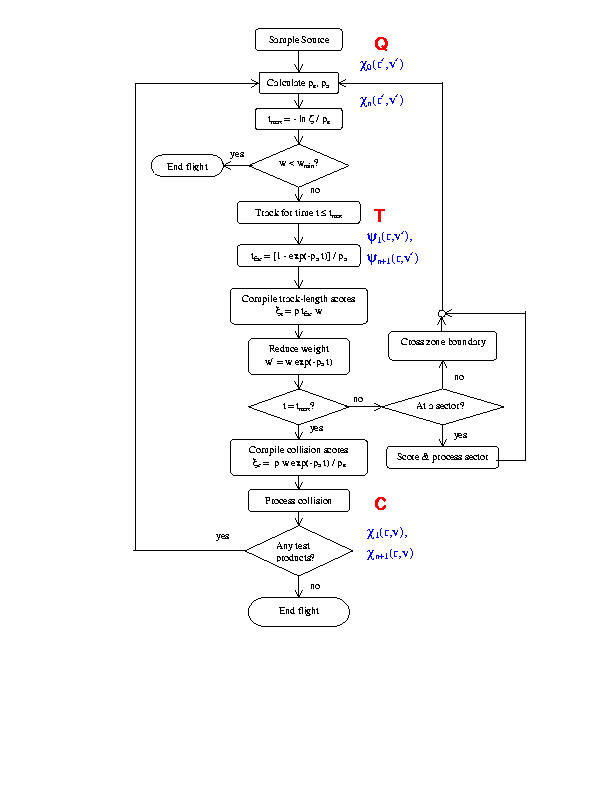
\includegraphics[width=6in]{flight_flowchart}
\vspace{-1.85in}
\caption{Flow chart of DEGAS 2 subroutine {\tt follow}, showing the steps 
involved in tracking a flight from its birth to its termination. Note
the weight reduction, and collision and tracklength estimators 
(Sec.~\ref{Estimators}). The operators from the integral equations are
shown along with the pre- and post-collision densities. These labels 
tie the practical algorithmic operations to the equations in 
Sec.~\ref{IntegralEquationDetails}. Some details have been omitted
for clarity.}
\label{flightflowchart}
\end{center}
\end{figure}

The flight is initiated as it is sampled from the spatial and velocity 
distribution of a source. Conceptually, this step amounts to
specifying $\chi_{0}(\vec{r}^{\prime},\vec{v}^{\prime},i)$ using the
source term $Q(\vec{r}^{\prime},\vec{v}^{\prime})$. The subscript
$0$ denotes the initial track for the flight. 

The next stage of the algorithm involves computing the reaction
rates $\rho_{s}$, $\rho_{a}$, etc. for the flight. Continuing
flights which require a recomputation (due to crossing from one
plasma region to another or to a change in species or velocity)
repeat the main loop starting at this same point. The 
post-collision density $\chi_{n}$
in Fig.~\ref{flightflowchart} is intended to refer to them.

The time to the next collision is randomly sampled 
(Sec.~\ref{SamplingDistance}) from the sum of the non-absorbing
reaction rates using a random number $\zeta$.

The weight $w$ is compared with some minimum weight to guarantee
that the flight terminates at some point. The ``End flight''
process indicated in Fig.~\ref{flightflowchart} actually represents
a Russian Roulette procedure\cite{Span69} which may allow the flight
to live a little longer.

The transport kernel $T$ translates the flight from position
$\vec{r}^{\prime}$ to $\vec{r}$. At the same time, this step 
represents the conceptual transition from post-collision density
to pre-collision density $\psi$, Eq.~(\ref{post2pre}). The tracking 
algorithm stops when $t = t_{\rm max}$, the flight
crosses a zone boundary (denoting a change in plasma parameters), or
a ``sector'' (a material or diagnostic surface; these will be
discussed later in this document) is reached. If a zone boundary
is crossed, the flight continues as is, although the rates must
be recomputed. Processing a sector may result in the continuation or the
termination of the flight, depending on the type of sector. Again,
the details have been omitted for simplicity.

If the flight reaches $t = t_{\rm max}$, the implication is that
it has had a collision. A particular collision is randomly chosen from 
amongst those possible for this particular flight.
At this point, precollision scores are recorded
and the collision itself is processed. Conceptually, this represents the
transition via the operator $C$ from $\psi_{n+1}$ to $\chi_{n+1}$.
If the reaction chosen results in no particles to track (e.g., 
in no neutral species; particles which DEGAS 2 has been instructed
to track are called ``test'' particles), the flight is terminated.
Test particles resulting from the collision are tracked in the same
manner, starting with the computation of the reaction rates.

\section{Atomic Physics}
\label{AtomicPhysics}
\index{Atomic physics}
\index{collisional-radiative}
\index{ionization}
\index{recombination}
\index{rates, atomic physics}

The interaction of electrons with hydrogen atoms and ions in a divertor
plasma is complicated by having comparable collision and radiative
decay times. The techniques for treating such systems were first 
described by Bates and McWhirter\cite{Bate61,McWh65}. The physical
processes included in such a collisional-radiative model are:
  \begin{enumerate}
    \item Electron collisional excitation $K_{e,mn}$ and de-excitation
$K_{d,mn}$,
    \item Spontaneous radiative transitions $A_{mn}$,
    \item Electron collisional ionization $K_{i,mn}$,
    \item Three-body recombination $K_{r,mn}$,
    \item Radiative recombination $\beta_{m}$,
\end{enumerate}
where $m$ and $n$ are principal quantum numbers. For the two state
terms, the initial state is the {\em second} number; the final is the
{\em first}. This apparently backward notation allegedly has a mathematical
origin.

A set of $m$ equations describes the balance between these processes that
determines the density of the $m$ -th excited state of the atom,
$N_{m}$,
\begin{eqnarray}
\frac{d N_{m}}{d t} & = & - N_{m} \left[ n_{e} \left( K_{i,m} + \sum_{n > m}
K_{e,nm} + \sum_{n < m} K_{d,nm} \right) \right. \nonumber \\
& & \qquad \quad \left. + \sum_{n < m} A_{nm} \right] \rule[-1ex]{0ex}{4ex} \nonumber \\
& & \quad + n_{e} \left( \sum_{n > m} N_{n} K_{d,mn} + \sum_{n < m} N_{n} K_{e,mn} 
\right) \rule[-2ex]{0ex}{4ex} \nonumber \\ & & \quad + \sum_{n > m} N_{n} A_{mn} + n_{e} n_{i} ( \beta_{m} + n_{e}
K_{r,m} ),
\end{eqnarray}
where $n_{e}$ is the electron density and $n_{i}$ is the density of ions
corresponding to the atom under consideration ($m \rightarrow \infty$,
effectively).

The basic assumption of the collisional-radiative model\cite{Bate61,McWh65}
is that states above ground state will decay much more rapidly than
the ground state will change. 
The evolution of the ground state is considered to be comparable to
the transport time scales. This physical process is the one considered by
the neutral transport code. In other words, the $m = 1$ equation will
essentially be solved by DEGAS 2 and $N_{1}$ can be treated as an
externally known quantity. The relatively rapid equilibration of the
excited states permits the time derivatives of their densities
to be set to zero. The set of equations for $m > 1$ can then be
solved,
\begin{equation}
N_{m} = \left( \frac{N^{(i)}_{m}}{N_{1}}\right) N_{1} + 
\left( \frac{N^{(ii)}_{m}}{n_{i}}\right) n_{i}.
\label{crnm}
\end{equation}
In practice, the solution of these equations involves:
\begin{enumerate}
  \item Obtaining the various reaction rates,  $K_{e,mn}$,
$K_{d,mn}$, $A_{mn}$, $K_{i,mn}$, $K_{r,mn}$, $\beta_{m}$,
as a function of $n_{e}$ and $T_{e}$,
  \item Solving the $m > 1$ equations for each $n_{e}$, $T_{e}$
pair with $N_{1} = 1$ and
$n_{i} = 0$, providing the ``coupling to the ground state'',
  \item Solving the equations again with $N_{1} = 0$ and
$n_{i} = 1$, yielding the ``coupling to the continuum''.
\end{enumerate}
Tables of $N^{(i)}_{m}/N_{1}$ and
$N^{(ii)}_{m}/n_{i}$ are thus obtained as a function of $n_{e}$ and
$T_{e}$.

With Eq.~(\ref{crnm}), the $m = 1$ equation can becomes
\begin{equation}
\frac{d N_{1}}{d t} = - N_{1} n_{e} S_{eff} + n_{e} n_{i} R_{eff} + {\rm
transport, etc.},
\end{equation}
with
\begin{equation}
S_{eff} = \sum_{m \geq 1} \left( \frac{N^{(i)}_{m}}{N_{1}}\right) K_{i,m},
\end{equation}
and
\begin{equation}
R_{eff} = - \sum_{m \geq 2} \left( \frac{N^{(ii)}_{m}}{n_{i}}\right) K_{i,m}
+ \sum_{m \geq 1} \left( \beta_{m} + n_{e} K_{r,m} \right).
\end{equation}
$S_{eff}$ is thus the effective ionization rate of the ground state
neutral, incorporating the multi-step processes associated with all
of the excited states. Likewise, $R_{eff}$ is the effective recombination
rate. Both are functions of $n_{e}$ and $T_{e}$ and are tabulated
along with selected values of the $N^{(i)}_{m}/N_{1}$ and
$N^{(ii)}_{m}/n_{i}$ for use in DEGAS 2.

Excited state densities, e.g., for $n = 3$, are found with
\begin{equation}
N_{3} = \left( \frac{N^{(i)}_{3}}{N_{1}}\right) N_{1} + 
\left( \frac{N^{(ii)}_{3}}{n_{i}}\right) n_{i}.
\end{equation}
Thus, 
the H$_{\alpha}$ emission rate is given by 
$N_{3} A_{23} = 4.41 \times
10^{7} N_{3}$ cm$^{-3}$ s$^{-1}$.

\subsection{Electron Energy Exchange Rate}

The expression used in {\tt collrad} for the electron energy exchange
is
\begin{eqnarray}
\frac{d E_{e}}{d t} & = & {\rm Ry} \left( - N_{1} n_{e} S_{eff} + 
n_{e} n_{i} R_{eff}  \right) \nonumber \\
& & \qquad - {\rm Ry} \sum_{\stackrel{m,n}{\scriptstyle n < m}} N_{m} A_{nm}
\left( \frac{1}{n^{2}} - \frac{1}{m^{2}} \right) \nonumber \\
& & \qquad - n_{e} n_{i} 
\sum_{m \geq 1} \beta_{m} \left( \langle E_{rad,m} \rangle + \frac{\rm Ry}{m^{2}}
\right),
\label{creloss}
\end{eqnarray}
where
\begin{itemize}
  \item Ry = 13.6 eV (one Rydberg),
  \item the first term is the loss due to ionization,
  \item the second is the gain due to recombination. 
  \item The sums represent lost photons from radiative transitions and
radiative recombination,
  \item $\langle E_{rad,m} \rangle$ is the average energy of a recombining 
electron.
\end{itemize}
For the last item, we use the expression given by Reiter\cite{Reit93},
\begin{equation}
\langle E_{rad,m} \rangle  =  T_{e} \left[ \frac{3}{2} 
   + \frac{T_{e}}{\beta_{m}} \frac{ d \beta_{m}}{d T_{e}} \right].
\end{equation}

Using Eq.~(\ref{crnm}), Eq.~(\ref{creloss}) becomes
\begin{equation}
\frac{d E_{e}}{d t} = - {\rm Ry} \left( N_{1} n_{e} S_{eff} - 
n_{e} n_{i} R_{eff}  \right) - N_{1} E_{loss}^{(i)} - n_{i} E_{loss}^{(ii)},
\end{equation}
where the terms $E_{loss}^{(i)}$, $E_{loss}^{(ii)}$ represent the loss
rates due to coupling to the ground state and continuum, respectively.
Both are provided as tables as functions of $n_{e}$ and $T_{e}$ for
use in DEGAS 2.

\subsection{Solutions Used with DEGAS 2}

The code we use to solve these equations, {\tt collrad}, 
is based on the one described
by Weisheit\cite{Weis75}. Rather than using Eq.~(\ref{crnm}), the original
code used the assumption that ionization and recombination were in balance 
to determine the neutral density in terms of the ion density.  The other
change made to Weisheit's version of the code is that the cross section
data have been updated as prescribed in the Janev-Smith database\cite{Jane93}.
The resulting collisional-radiative data are believed to be
in good agreement with ADAS. Although the {\tt collrad} code is not
itself distributed with DEGAS 2, it can be obtained from the DEGAS 2
authors (see Sec.~\ref{help}).

The output data from {\tt collrad} are contained in the file {\tt ehr2.dat}.
(contains...) Earlier versions of this same file, {\tt eh.dat} 
(as generated by Weisheit's original code) and {\tt ehr1.dat}
[generated with Weisheit's code modified to use Eq.~(\ref{crnm})] are
also included in the DEGAS 2 distribution since they were both used 
extensively with the original DEGAS code.

The {\tt ehr2.dat} file contains
\begin{enumerate}
  \item Ionization rate $S_{eff}$ in cm$^{3}$ s$^{-1}$,
  \item Recombination rate $R_{eff}$ in cm$^{3}$ s$^{-1}$,
  \item Neutral electron losses $E_{loss}^{(i)}$ in erg s$^{-1}$,
  \item Continuum electron losses $E_{loss}^{(ii)}$ in erg s$^{-1}$,
  \item Neutral ``n=3 / n=1'', $N_{3}^{(i)} / N_{1}$,
  \item Continuum ``n=3 / n=1'', $N_{3}^{(ii)} / n_{i}$,
  \item Neutral ``n=2 / n=1'', $N_{2}^{(i)} / N_{1}$,
  \item Continuum ``n=2 / n=1'', $N_{2}^{(ii)} / n_{i}$.
\end{enumerate}
The portion of the file for each quantity consists of 15 separate sections 
(labeled by {\tt jn}), corresponding to the various electron density values,
\begin{equation}
n_{e}({\tt jn}) =  10^{10 + ({\tt jn} - 1)/2} \: {\rm cm}^{-3}.
\end{equation}
Each section consists of 60 data values, one for each $T_{e} ({\tt jt})$,
\begin{equation}
T_{e}({\tt jt}) =  10^{-1.2 + ({\tt jt} - 1)/10} \: {\rm eV}.
\end{equation}
The index {\tt jt} starts at 1 in the first column and row and proceeds 
row-by-row. There are 10 rows of 6 entries each.

\section{Elastic Scattering}
\label{ElasticScattering}
\index{Elastic scattering}

\subsection{Neutral-Ion Elastic Scattering}
\label{NeutralIon}
\index{Neutral-ion scattering}
\index{Charge exchange}
\index{Spin exchange}
\index{Diffusion cross section}
\index{Total cross section}
\index{Viscosity cross section}
\index{Scattering angle}
\index{Differential cross section}

{\em Note: this subsection was extracted from Ref.~\cite{Kanz00}. 
A few minor changes in notation have been made for consistency.}
Only limited experimental data are available for ion-neutral elastic
scattering at low energies.  The monograph by Janev\cite{Jane87} is one of the
most widely used data sources available, but only contains charge
exchange at moderate to high collision energies and no data for
elastic scattering.  As divertor technology has progressed, low
temperature operating environments have become a standard mode of
operation.  Under these conditions, both charge exchange and
small-angle elastic scattering must be included in simulations.  Below
approximately 2 eV for $D^{+} + D$ collisions, separate treatment of
small-angle elastic scattering and resonant charge exchange becomes
impossible due to quantum mechanical effects.  The need for a
comprehensive treatment of ion-neutral elastic collisions at low
energies motivated the \href{http://www-cfadc.phy.ornl.gov/}{Controlled Fusion Atomic Physics Data Center} at
ORNL to produce a collection of total differential elastic scattering
cross sections for 31 various isotopic combinations of hydrogen atoms
and molecules\cite{Krst98}.

DEGAS 2 represents an improvement over the
original DEGAS code in that the pseudo-collision algorithm originally
employed in scoring results\cite{Heif82} is replaced with a track-length type
estimator.  This allows efficient determination of momentum and energy
exchange with the background plasma over a wide range of background
densities.  The rate expressions used by the track-length estimator
involve the momentum transfer (or diffusion) 
cross section, $\sigma_{d}$\cite{Bach95}.

A general
expression for the integral cross sections is\cite{Bach95}
\begin{equation}
\sigma_{l} = 2 \pi \int_{0}^{\pi} \left( 1 - \cos \theta \right)^{l}
\sigma(\theta, E_{r}) \sin \theta \: d \theta,
\label{sigmal}
\end{equation}
where $l=0$
corresponds to the total elastic scattering cross section, $l=1$ to the
diffusion cross section and $l=2$ to the viscosity cross
section; $\theta$ is the center-of-mass scattering angle, $E_{r}$ 
is the relative
energy of the collision, and $\sigma(\theta,E_{r})$ is the differential elastic
scattering cross section.  The total elastic collision cross section,
$\sigma_{t}$, is used in Monte Carlo simulations to determine the time between
elastic collisions.  In this manner the size of the total elastic
collision cross section influences the execution time of numerical
simulations.

A simulation technique that reduces the total
collision cross section while keeping the momentum transfer cross
section invariant can be developed.  Using the expression for $\sigma_{d}$ and
dividing Eq.~(\ref{sigmal}) into small and large angle components,
\begin{equation}
\sigma_{d} (E_{r}) = 2 \pi \int_{0}^{\theta_{\rm min}} C(E_{r})
( 1 - \cos \theta) \delta(\theta - \theta_{\rm min}) \: d \theta 
+ 2 \pi \int^{\pi}_{\theta_{\rm min}} 
( 1 - \cos \theta) \sigma(\theta, E_{r}) \: d \theta.
\label{sigmad}
\end{equation}
Substituting $\sigma(\theta,E_{r})$ from the ORNL data set here and directly
computing $\sigma_{d}(E_{r})$  [via Eq.~(\ref{sigmal})], 
allows Eq.~(\ref{sigmad}) to be solved for
$C(E_{r})$ given a particular value of $\theta_{\rm min}$.  
The resulting value of $C(E_{r})$
is then used in a similar expression for the viscosity cross section.
This provides viscosity cross sections accurate to second order in
$\theta_{\rm min}$.  The value of $\theta_{\rm min}$ 
is chosen so as to reduce the total elastic
cross section as much as possible while retaining physical realism.

For low energy elastic collisions a significant portion of the
collisions involve small-angle deflections.  Due to this behavior, the
majority of the reduction in total elastic cross section is obtained
with a five-degree minimum scattering angle (Fig.~\ref{rjkfig1}).  Minimum
scattering angles greater than five degrees result in little
computational savings.  The resulting reduction in $\sigma_{t}$ 
is approximately
a factor of two at relative energies $E_{r} > 10^{-1}$ eV.  The values for 
$\sigma_{d}$
are unchanged during application of a small-angle cut-off. 

\begin{figure}
\begin{center}
\leavevmode
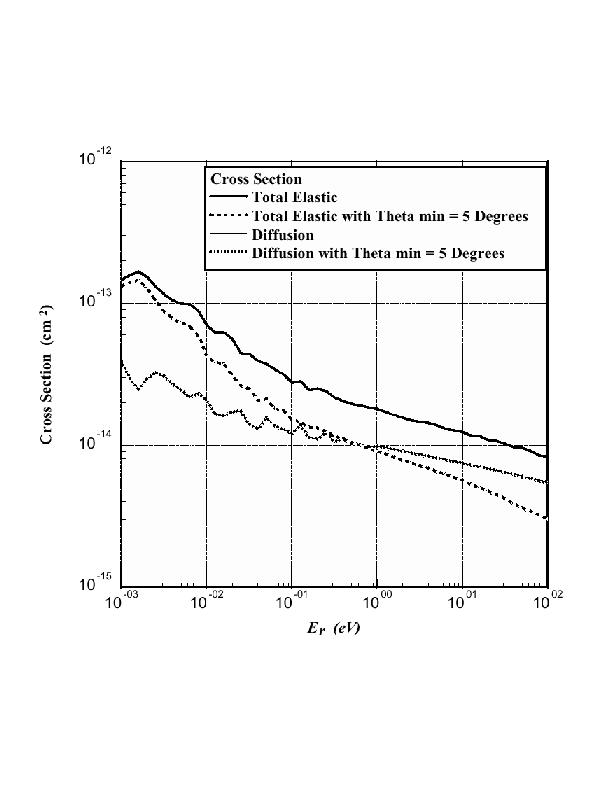
\includegraphics[width=5in]{rjk_fig1}
\caption{Comparison of total and diffusion cross sections for $D^{+} + D$
collisions with and without the small-angle cut-off approximation.}
\label{rjkfig1}
\end{center}
\end{figure}

The
use of this small-angle cut-off leads to an efficient algorithm for
simulating the dynamics of elastic collisions in Monte Carlo
simulations.  Previous models based on classical collision kinetics
for direct elastic scattering face difficulties in that the cross
section is a rapidly varying function of the impact parameter\cite{Bach95}.  
This
precludes the use of efficient table-look-up methods and forces a time
consuming evaluation of the collision integral for each individual
interaction.

Utilization of the differential elastic cross
section, $\sigma(\theta,E_{r})$, 
allows development of a table-look-up interpolation
for both direct elastic scattering and resonant charge exchange.
Following the work by Abou-Gabal and Emmert\cite{Abou91}, 
we divide the total
elastic cross section into $n$ pieces and interpret the result as a
cumulative probability distribution function,
\begin{equation}
P_{i} = 2 \pi \int_{-1}^{\cos \Theta_{i}} 
\frac{\sigma(\theta, E_{r})}{\sigma_{t}(E_{r})} \: d( \cos \theta),
\: i = 0, 1, \ldots n.
\label{scatprob}
\end{equation} 
Equation~\ref{scatprob}
is inverted to obtain the scattering angle as a function of relative
energy and $n$ equally spaced values of the cumulative probability
spacing, $\Theta_{i}(P_{i},E_{r})$, where $\Theta_{i}$ 
is the scattering angle in the
center-of-mass frame.  Examples of $\Theta_{i}(P_{i},E_{r})$
for the $D^{+} + D$ and $D^{+} + D_{2}$
collisions at a center-of-mass energy of 1 eV are presented in 
Fig.~\ref{rjkfig2}.
At this energy, inclusion of direct elastic scattering increases the
probability that colliding particles undergo small angle deflections.
Consideration of charge exchange alone would shift the probability
distribution to favor collisions resulting in $\Theta = \pi$.  As evident in
Fig.~\ref{rjkfig2}, $\Theta_{i}(P_{i},E_{r})$ for like-species 
collisions exhibits a higher
probability of undergoing large-angle collisions compared to the
ion-molecular collision case.  This is due to the absence of a charge
exchange contribution to the scattering function for ion-molecular
elastic collisions.  Monte Carlo collision processing begins with the
sampling of a suitable ion from a Maxwellian distribution at the local
ion temperature, yielding, $E_{r}$.  The $P_{i}$ 
are next sampled from a uniform
distribution.  The collision angle follows from a bi-linear
interpolation into this data table without evaluation of complex
integral functions.

\begin{figure}
\begin{center}
\leavevmode
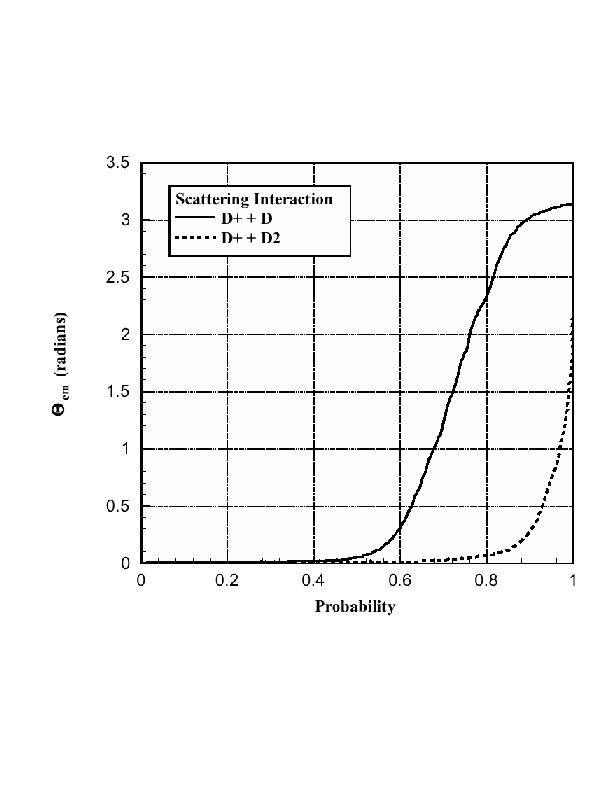
\includegraphics[width=5in]{rjk_fig2}
\caption{Scattering function $\Theta_{i}(P_{i},E_{r})$ for
$D^{+} + D$ and $D^{+} + D_{2}$ ion-neutral elastic
interactions at an interaction energy of 1
eV.}
\label{rjkfig2}
\end{center}
\end{figure}

Previous treatments of charge exchange in
Monte Carlo algorithms employed a $180^{\circ}$ collision scattering model in
the center-of-mass frame.  The approach is simple to implement,
requiring just the exchange of the ion and neutral velocity vectors
and yields a momentum transfer cross section of about $2 \sigma_{cx}$, 
where $\sigma_{cx}$
is the charge exchange cross section.  This is, in fact, roughly equal
to the total diffusion cross section in ion-neutral
collisions, $\sigma_{d} \sim 2 \sigma_{cx}$ \cite{Dalg58,Hols52,Wade79}
The accuracy of this simple
expression is demonstrated in Fig.~\ref{rjkfig3}, which compares the 
diffusion cross section with results for the ``spin exchange'' cross
section from the ORNL data\cite{Krst98}.  
Spin exchange is defined as the exchange
of the intrinsic quantum mechanical property of particle spin; for
distinguishable particles this is equivalent to charge exchange.  For
like-species collisions, spin exchange and charge exchange are 
equivalent only within classical regimes.  The relation 
$\sigma_{d} \sim 2 \sigma_{cx}$
holds within the classical regime above approximately 2 eV for $D^{+} + D$.
At lower energies, the particles must be treated as indistinguishable
and separation of direct elastic scattering and charge exchange is no
longer possible.  At these low energies, spin exchange is no longer
equivalent to charge exchange and the relation 
$\sigma_{d} \sim 2 \sigma_{cx}$ no longer
holds.  This illustrates the difficulties in treating ion-neutral
elastic collisions by charge exchange alone under low-temperature
detached conditions.

\begin{figure}
\begin{center}
\leavevmode
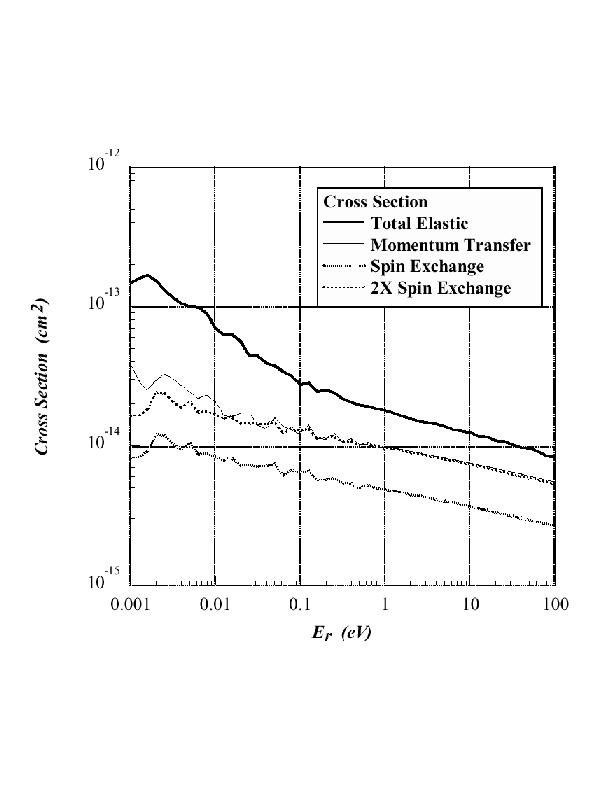
\includegraphics[width=5in]{rjk_fig3}
\caption{Comparison of diffusion and charge exchange cross sections for 
$D^{+} + D$ elastic collisions.}
\label{rjkfig3}
\end{center}
\end{figure}

\subsection{Neutral-Neutral Elastic Scattering}
\label{NeutralNeutral}

\subsection{Validation of BGK Model and Rates}
\label{BGKRates}
\index{BGK}
\index{Viscosity}
\index{Diffusion}
\index{Neutral-neutral scattering}
\index{Maxwell molecules}

As described by May\cite{Mayxx}, the reaction rates for the BGK algorithm
can be determined by matching physical quantities, the viscosity and
diffusion cofficients, against measured values. However, since the May's
work and the publication of Reiter\cite{Reit97}, the ORNL 
CFADC has
computed \href{http://www-cfadc.phy.ornl.gov/elastic/elastic0.html}{differential scattering cross sections} \cite{Krst98}, analogous to those
described in Sec.~\ref{NeutralIon}, for these neutral-neutral systems.
In this subsection we will show that the two approaches are largely
consistent, at least near room temperature.

We proceed in a manner analogous to May. Namely, we will obtain from the
CFADC differential cross sections values for the viscosity and diffusion
coefficients. Using the same expressions as May, these will be transformed
into reaction rates that can be compared with those described in 
Sec.~\ref{NeutralNeutral}.

For self-collisions, we consider the viscosity. The general expression 
derived in Chapman and Cowling\cite{Chap70} [their Eq.~(10.1,4)] is
\begin{equation}
\mu_{1} = \frac{5}{8} \frac{k T}{\Omega_{1}^{(2)}(2)},
\label{visc1}
\end{equation}
where $\Omega_{1}^{(l)}{(n)}$ corresponds directly to the $\Omega^{l,n}$
integrals described by Bachmann\cite{Bach95}.  The subscript ``1'' here 
is to be associated with the cross section and refers to collisions of species 
``1'' with itself (as opposed to collisions between species ``1'' and 
``2'' which will be labeled with ``12'' below).

Likewise, we have for the diffusion coefficient [Eq.~(9.81,1) in
Ref.~\cite{Chap70}],
\begin{equation}
D_{12} = \frac{3}{16} \frac{k T}{(n_{1} + n_{2})m_{r} \Omega_{12}^{(1)}(1)},
\label{diff1}
\end{equation}
where $n_{1}$ and $n_{2}$ are the species densities and $m_{r}$ is the
reduced mass for the system, $m_{r} = m_{1} m_{2} / (m_{1} + m_{2})$.

The $\Omega^{(l)}(n)$ integrals represent averaging of the collision 
cross sections over Maxwellian distributions for both species. The
{\tt ratecalc} code is able to integrate these cross sections over
a single Maxwellian distribution,
namely, the $I_{l,n}$ described in Reiter\cite{Reit93}
and the \href{ratecalc.pdf#page.3}{documentation} for {\tt ratecalc}.
Fortunately, the double integral can be found as a limiting case of 
the single integral:
\begin{equation}
\langle I_{l,n} \rangle(u_{p},u_{n}) = \lim_{u^{\prime} \rightarrow 0} 
I_{l,n}(u_{p}^{\prime},u^{\prime}),
\label{Iln1}
\end{equation}
where $u_{p}^{\prime 2} \equiv u_{p}^{2} + u_{n}^{2}$, and 
$u_{p} = \sqrt{2 T_{p} / m_{p}}$ is the thermal velocity of the
second species. Likewise, $u_{n} = \sqrt{2 T_{n} / m_{n}}$ is the
thermal velocity associated with the Maxwellian distribution used in the
averaging over $u$.  The $\langle I_{l,n}\rangle$ is then related to
$\Omega^{(l)}(n)$,
\begin{equation}
\langle I_{l,n} \rangle = 8 \left( \frac{u_{p}^{\prime}}{u_{p}} \right)^{n}
\Omega^{(l)}(n/2).
\label{Iln2}
\end{equation}
The same result is quoted in Ref.~\cite{Bach95} and in \cite{Reit93},
although in the latter case the variable equivalent to $u_{p}^{\prime}$
is incorrectly defined.

With these expressions, we can compute the single species viscosity and
two species diffusion coefficients from the CFADC differential scattering
cross sections. The corresponding expressions for the ``Maxwell molecule''
interaction [intermolecular force given by $\kappa / r^{5}$; e.g., see
Eq.~(12.1,1) in Ref.~\cite{Chap70})] are
\begin{equation}
\mu_{1} = \frac{k T}{3 \pi A_{2}(5)} \sqrt{\frac{2 m}{\kappa}},
\label{visc2}
\end{equation}
where $A_{2}(5) = 0.436$ is the result of a dimensionless integral.
And from Eq.~(14.2,2) of Ref.~\cite{Chap70},
\begin{equation}
D_{12} = \frac{k T}{2 \pi A_{1}(5)} \frac{1}{n \sqrt{\kappa_{12} m_{r}}},
\label{diff2}
\end{equation}
where $A_{1}(5) = 0.422$ is the result of another dimensionless integration.

The reaction rates needed for the BGK algorithm are related to the constant
in the Maxwell molecule force law by (see Ref.~\cite{Mors63} or \cite{Mayxx}),
\begin{equation}
\langle \sigma v \rangle_{11} = 2 \sqrt{2} \pi A_{1}(5)
\sqrt{\frac{\kappa}{m}},
\label{sv11}
\end{equation}
and 
\begin{equation}
\langle \sigma v \rangle_{12} = 2 \pi A_{1}(5)
\sqrt{\frac{\kappa_{12}}{m_{r}}}.
\label{sv12}
\end{equation}

Now, we can use Eq.~(\ref{visc2}) to eliminate $\kappa$ in Eq.~(\ref{sv11})
in favor of $\mu_{1}$. Then, we can insert  $\mu_{1}$ as given by
Eq.~(\ref{visc1}) to obtain an effective BGK reaction rate that has the
same viscosity as that computed directly from the CFADC differential
cross sections:
\begin{equation}
\langle \sigma v \rangle_{11} = 2.065 \Omega_{1}^{(2)}(2).
\end{equation}
The analogous procedure for the diffusion coefficient yields
\begin{equation}
\langle \sigma v \rangle_{12} = \frac{16}{3} \Omega_{12}^{(1)}(1).
\end{equation}

Finally, we can use Eqs.~(\ref{Iln1}) and (\ref{Iln2}) to
replace the $\Omega$ integrals with the equivalent integrals obtainable
from {\tt ratecalc},
\begin{equation}
\langle \sigma v \rangle_{11} = \frac{2.065}{32} 
\lim_{u^{\prime} \rightarrow 0} I_{2,4} (u_{p}^{\prime} = \sqrt{2} u_{p},
u^{\prime}),
\end{equation}
and
\begin{equation}
\langle \sigma v \rangle_{12} = \frac{2}{3} 
\frac{u_{p}^{2}}{u_{p}^{2} + u_{n}^{2}} 
\lim_{u^{\prime} \rightarrow 0} I_{1,2} 
(u_{p}^{\prime} = \sqrt{u_{p}^{2} + u_{n}^{2}}, u^{\prime}).
\label{sv122}
\end{equation}

In evaluating the latter expression, we will assume that one of the
species (e.g., molecules at the wall temperature) are much cooler
than the other, i.e., $u_{n} \ll u_{p}$. Equation~(\ref{sv122}) then
becomes a function of only $u_{p}$.

The CFADC data exist only for the $D + D_{2}$ and $D + D$ systems 
(and isotopic equivalents; molecules are computationally intensive, hence,
the absence of molecule-molecule data). These are compared with the 
May data in Fig.~\ref{scattering}. 

One concern with May's treatment of the $D + D$ case is that the 
empirical viscosity formula quoted in Ref.~\cite{Mayxx} does not
appear in the literature, nor is its origin clearly stated. The best
guess for its origin is that it was obtained by rescaling the 
``Fuller'' expression for the diffusion coefficient\cite{Reid87}
into a viscosity using the theoretical expressions to relate the two.
In Fig.~\ref{viscosities}, we compare May's expression with two that do
appear directly in Ref.~\cite{Reid87} (``Chung'' and ``Lewis'') and with
individual data points listed in the CRC Handbook\cite{CRC}.  The 
agreement of these values near room temperature ($\sim 0.03$ eV) is
expected. However, May's formula has a stronger temperature scaling than
the others and exceeds them by about a factor of 15 at 10 eV. The
relevant temperature range for this process is expected to be between
1 and 10 eV.

Figure~\ref{scattering} shows that at least near room temperature,  
May's expressions are also consistent with the CFADC data. However,
in the 1 to 10 eV range, they are considerably larger than the
CFADC values,
suggesting that the values used in DEGAS 2 (and EIRENE) may be too
large.

\begin{figure}
\begin{center}
\leavevmode
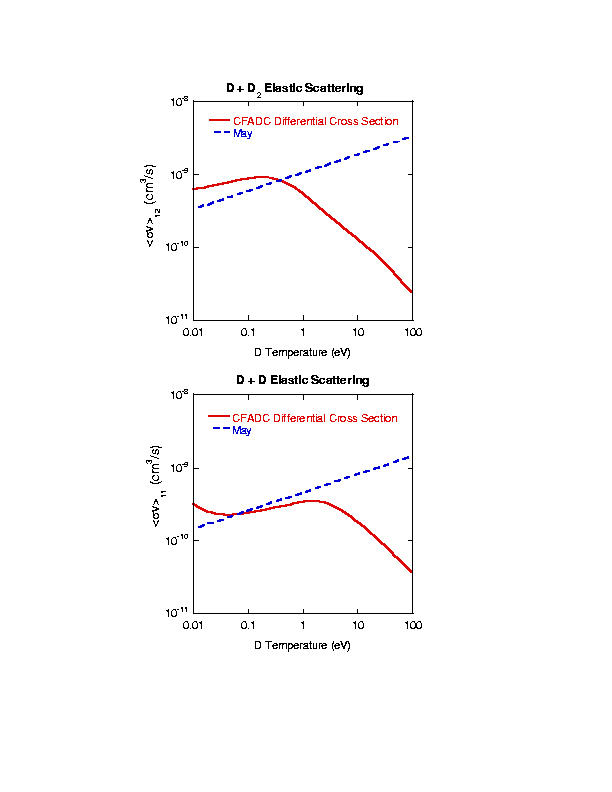
\includegraphics[width=5in]{scattering_plot}
\caption{Comparison of reaction rates for the $D + D_{2}$ and $D + D$ 
systems.  The original rates suggested by May\cite{Mayxx} and effective
rates computed from the CFADC data are shown.}
\label{scattering}
\end{center}
\end{figure}

\begin{figure}
\begin{center}
\leavevmode
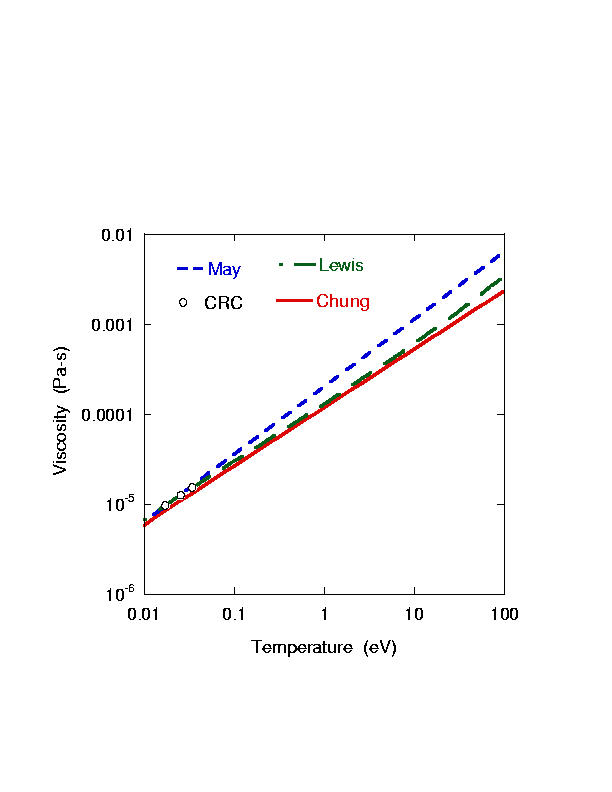
\includegraphics[width=5in]{viscosity_plot}
\caption{Comparison of viscosity formulas from May\cite{Mayxx}, 
Reid{Reid87} (the ``Chung'' and ``Lewis'' expressions), and the CRC
Handbook\cite{CRC}.}
\label{viscosities}
\end{center}
\end{figure}

\chapter{Structure of DEGAS 2}

The essential inputs to a Monte Carlo neutral transport code are:

\begin{itemize}
\item The neutral or test species which are of interest,
\item The species and phase space distribution of the background 
species with which
the test species will interact, 
\item The interaction processes between the test and background species. 
The relative probability of these processes as a function of the 
test and local background properties are required as well as a 
prescription for specifying the outcome of each interaction.
\item The simulation geometry, including a framework for
holding the background species data, as well as a means for tracking
the test species through the background.
\item The boundaries of the geometry, including a prescription
for specifying the outcome of interactions between the test species and
these boundaries.
\end{itemize}

In this chapter we will familiarize the user with way these inputs are 
defined and specified for DEGAS 2, as well as provide an overview 
of the rest of the code. More
detailed information on running DEGAS 2 will follow in later chapters.

\section{Structure of the File System}

Here is an example structure of the directories under the top-level 
{\tt degas2} directory. Those labeled with ``(D)'' represent
source and data directories maintained with CVS. The others are created
by the user as described in the compiling section.

\begin{description}
\item[data] Input atomic and surface physics data and information (D)
\item[src] All source code (D)
\item[Doc] Location of the various formats of this document and ancilliary
files (needs to be established in archive)
\item[examples] Input and output files from example and benchmark runs 
\item[Aladdin] Source code and data for use with IAEA Aladdin package (D)
\item[ALPHA] Object and executable files for Dec Alpha machines
\item[SUN] Object and executable files for Sun Solaris and SunOS machines
\item[CRAY] Pre-processed source code for export to Cray computers
\item[tex] Intermediate files and final DVI documentation files generated 
from source code
\end{description}

\section{Components of the Code}
\label{components}

DEGAS 2 is not a single code (not now anyway), but a complex package of 
setup, test, simulation, and post-processing tools. Which ones are
needed depend on the user's objectives and familiarity with DEGAS 2.
A few additional ``targets'' are listed in the Makefile. These are
either sufficiently out of date or infrequently used to warrant
mention here.

\subsection{Main Code}
\label{maincode}
\index{problemsetup}
\index{readgeometry}
\index{readbackground}
\index{tallysetup}
\index{flighttest}
\index{geomtesta}

Virtually every user will be running these executables,
usually in this order.

\begin{description}
\item[problemsetup] Reads a text file describing the species, 
materials, atomic, and surface physics required for the
current problem. The code
accesses the required "reference" data, and compiles them
into a netCDF file (the {\tt problem.nc} file).
\item[readgeometry] Generates a DEGAS 2 netCDF geometry file from an
existing DEGAS, UEDGE, or SONNET geometry description. Hopefully, this
package will be superseded by other more general means of generating
geometries (and backgrounds). A short text input file helps readgeometry
through the transformation process.
\item[readbackground] Plasma data in an external file is mapped onto
the zones of the DEGAS 2 geometry. Presently, only DEGAS and UEDGE files
can be used; readgeometry and readbackground read the same data
file. 
\item[updatebackground] Is similar to readbackground, but is intended
for use in iterations with the UEDGE code {\em only}. The source
information generated by the initial run of readbackground is 
stored in a separate file ({\tt oldsourcefile},
Sec.~\ref{degas2in}). On subsequent
iterations, small changes in the source terms are accounted for
by allowing non-unit weighting factors at each source segment.
Once the accumulated changes exceed a certain size (specified by
parameters in the sources class), the DEGAS 2 source sampling
arrays are re-initialized (i.e., to once again use unit weights)
and the {\tt oldsourcefile} is rewritten. The effectiveness of this
procedure is currently being evaluated and should be considered
as experimental.
\item[tallysetup] This code specifies the types of ``scores'' (the
essential output of the code), along with their
dependencies, which will be computed in the DEGAS 2 run. Although the input
files(s) should not be modified by the novice user, this code needs to be
run to factor the values of physics and geometry parameters for the
problem at hand into the specification of these scores.
\item[flighttest] The core of DEGAS 2. This program launches, follows,
and scores the Monte Carlo trajectories which make up a DEGAS 2 simulation.
(The name is a holdover from early versions in which this did tracking 
with a minimum of hardwired physics).
\item[outputbrowser] Reads the output netCDF file generated by
{\tt flighttest} (in addition to all other netCDF files for the
problem) and allows the user to interactively browse its contents.
A script facility is provided for batch-like operation. 
\item[geomtesta] Another inappropriately named routine which serves as
the principal post-processing cdoe for DEGAS 2. Although originally
designed as a diagnostic for the geometry, it has proven too easy to 
continue extending this code to warrant development of an honest
post-processing tool. The DEGAS 2 input and output files are read in by
the code. Using the geometry information, the zone-based plasma and neutral
data are transcribed onto a high density uniform rectangular mesh and
dumped into the HDF files suitable for further manipulation by commercial
products such as IDL and Noesys.
\end{description}

\subsection{Other Setup Routines}
\label{othersetup}
\index{datasetup}
\index{ratecalc}
\index{reactionwrite}
\index{pmiwrite}
\index{boxgen}

These are occasionally used to add new atomic
or surface physics reactions, or to generate new atomic and surface physics
data files.

\begin{description}
\item[datasetup] This routine possibly belongs in the first list. It
reads text files describing the complete lists of elements, species, reactions,
materials, and plasma-material interactions available to DEGAS 2 and generates
the corresponding DEGAS 2 netCDF files. These lists are occasionally referred 
to in the code as the "reference" lists; the input file for problemsetup
specifies subsets of these lists. A new reaction is added to DEGAS 2 by 
inserting the requisite information into the ``reactionfile'' 
and rerunning datasetup. The new reaction can
then be added to the problem input file.
\item[ratecalc] A routine for computing averages of atomic physics
cross sections. Since it is designed to read data from the Aladdin 
database, ratecalc is presently limited in its flexibility. The principal
application thus far has been the generation of reaction rates and higher
moments for charge exchange and other interactions between atoms, molecules,
and ions.
\item[reactionwrite] A simple routine designed to translate collisional
radiative data for the electron impact ionization of hydrogen from the
format used by the old DEGAS code into netCDF files (ionization and
recombination) for DEGAS 2. This code has been run a handful of times
as needed to keep up with changes in the content and format of the atomic
physics data files.
\item[pmiwrite] Is analogous to reactionwrite, but handles almost all
of the plasma-material interaction data. Presently, two data files from
the old DEGAS code and one from EIRENE are used as input. A few processes
describable without external data are also included. This code can be used,
in a somewhat clumsy manner, to add new plasma-material interaction data
to DEGAS 2 using either one of these three existing data bases or via
a new datafile (with the rest of the code serving as an example).
\item[boxgen] Is intended to serve as an example of how to generate
geometry and background files from scratch. As the name implies, boxgen
sets up a simple box geometry with a linearly varying plasma.
\end{description}

\subsection{Test Routines}
\label{testroutines}
\index{reactiontest}
\index{pmitest}
\index{sourcetest}
\index{dataexam}
\index{sysdeptest}
\index{randomtest}

\begin{description}
\item[reactiontest] Can be run after problemsetup to check the computation
of the reaction rate, and collision products (including velocities and
scoring data) for a given reaction.
\item[pmitest] The analog of reactiontest for plasma-material
interactions. Again, this code can be executed for a given problem once
problemsetup has been run. Since the velocity distributions of some
plasma-material interactions are described statistically, pmitest
is also set up to average the outcome of a given interaction over a
specified number of trials and print out a list of the product velocities
for external manipulation.
\item[sourcetest] Tests the distribution in phase space of the source
terms for a particular problem. Since the source is described in the 
``background'' netCDF file, readbackground, boxgen, or something equivalent
must be run prior to using this routine. Like pmitest, the code is able
to run many trials, compute averages, and printout data from each 
individual trial.
\item[dataexam] Provides the user with a convenient interface to the
atomic physics data files. Although netCDF files can be converted to
a human-readable text form, interpreting those data is since DEGAS 2
collapses the multi-dimensional structure components of the atomic physics data
into a single one-dimensional array. This routine reads the ``raw'' (at
the ``reference'' level) data files prior to their insertion into the
problem netCDF file and, thus, can be run at any time. An analogous
routine for the plasma material interactions is needed.
\item[sysdeptest] Tests several system-dependent features of DEGAS 2.
This would be run only if the code was being ported to a new operating
system or if the operating system on a currently supported architecture
underwent a signficant upgrade.
\item[randomtest] Is used to verify that DEGAS 2 will give the same 
results on 
different architectures (provided the random number seeds are set the
same!). 
\end{description}

\subsection{Miscellaneous Routines}
\label{miscroutines}
\index{matchout}
\index{matcheir}

\begin{description}
\item[matchout] Is used to compare the current DEGAS 2 output netCDF
file with another from an equivalent run (i.e., all of the arrays must
be exactly the same size). The most frequent use
of {\tt matchout} is to verify that two separate runs have yielded 
results which are the same to within roundoff error. Because of the size of 
the ouptut netCDF file, verifying this by visually comparing the files 
is impractical.  
\item[matcheir] Is specifically designed for comparing with output from
the EIRENE code. See Sec.(the same physics benchmark).
\end{description} 

\section{Input Files}

DEGAS 2 utilizes several text based input files for controlling the actions
of its component executables (see Sec.~\ref{components}).

\subsection{degas2.in}
\label{degas2in}
\index{symbolic name}

{\tt degas2.in} is the input file which controls (most of) the other
input files. Each line consists of DEGAS 2's symbolic name for the
file (this can be changed only by modifying {\tt readfilenames.hweb}
and {\tt readfilenames.web}) followed by the path name for the file
to be used in the current problem. The order of the lines in this file
is unimportant. Comments (beginning with \#) and spaces are ignored.

\begin{verbatim}
elementsfile  ../data/elements.nc 
backgroundfile bk_uers.nc 
testfile  test.nc 
geometryfile ge_uers.nc 
problemfile pr_uers.nc
reactionfile reactions.nc
speciesfile ../data/species.nc 
aladinfile ../data/aladinput.nc
aladoutfile ../data/aladoutput.nc 
elements_infile ../data/elements.input
problem_infile  pr_uers.input
reaction_infile reactions.input
species_infile ../data/species.input
materials_infile ../data/materials.input
materialsfile ../data/materials.nc
pmi_infile ../data/pmi.input
pmifile ../data/pmi.nc
cramdproblemfile cramdprob.nc
tallyfile tally_uers.nc
outputfile degas2_uers_out.nc
oldsourcefile os_uers.nc
\end{verbatim}

Note that some of these are 
outdated or rarely used (unused entries may be deleted from the file, if
desired). Most of the files come in pairs with the name
\verb+XXX_infile+ corresponding to a text input file and
\verb+XXXfile+ being a netCDF file generated by a program
like {\tt datasetup}, {\tt problemsetup}, etc.

\subsection{elements\_infile}
\label{elementsinfile}
\index{elements\_infile}
\index{elementsfile}

{\tt elements\_infile} lists all of the elements available to DEGAS 2 for
use in constructing the species (see Sec.~\ref{speciesinfile}). 
Additional detail is given at the beginning of the 
\href{elementsetup.pdf#page.1}{file} {\tt elementsetup.web}.

\subsection{species\_infile}
\label{speciesinfile}
\index{species\_infile}
\index{species}
\index{generic}
\index{speciesfile}

Inputs for species are contained in the file with the symbolic
name {\tt species\_infile}. Additional detail is given at the beginning
of the \href{speciesetup.pdf#page.1}{file} {\tt speciesetup.web}.

\subsection{reaction\_infile}
\label{reactioninfile}
\index{reaction\_infile}
\index{reaction type}
\index{chargex}
\index{elastic}
\index{dissoc}
\index{dissoc\_rec}
\index{ionize}
\index{ionize\_suppress}
\index{recombination}
\index{reactionfile}
\index{generic reactions}
\index{non-generic reactions}

The file {\tt reaction\_infile} describes all of the reactions available in
DEGAS 2. Additional detail is given at the beginning of the
\href{reactionsetup.pdf#page.1}{file} {\tt reactionsetup.web}.

Note that adding a new reaction to this file involves two tasks beyond 
inserting the appropriate lines in {\tt reaction\_infile}. First, the 
netCDF file for the atomic physics data must be generated (see
Sec.~\ref{addreactions}). The
second task would be to write subroutines for setting up the products and
handling collisions (see Sec.~\ref{reactionprocessing}). 
This would be necessary only if a new reaction type
were being added.

\subsection{materials\_infile}
\label{materialsinfile}
\index{materials\_infile}
\index{materialsfile}

The materials described in {\tt materials\_infile} are essentially just labels
which will be used in conjunction with the plasma material interactions 
(see Sec.~\ref{pmiinfile}) to specify how test 
species interact with non-transparent
surfaces. Additional detail is given at the beginning of the 
\href{materialsetup.pdf#page.1}{file} {\tt materialsetup.web}.

\subsection{pmi\_infile}
\label{pmiinfile}
\index{pmi\_infile}
\index{PMI}
\index{generic PMI}
\index{non-generic PMI}
\index{reflection}
\index{adsorption}
\index{desorption}

The file {\tt pmi\_infile} describes all of the plasma-material interactions
(PMI) available in DEGAS 2. Additional detail is given at the beginning
of the \href{pmisetup.pdf#page.1}{file} {\tt pmisetup.web}.

\subsection{problem\_infile}
\label{probleminfile}
\index{reference level}
\index{subset data}
\index{test species}
\index{background species}
\index{problem\_infile}
\index{problemfile}

As noted already in the section describing the DEGAS 2 components
(see Sec.~\ref{components}), there are two levels of physics input to DEGAS 2.
The input files noted thus far comprise the reference level: in
practice, the sum total of the data available to the code (although
in principle it could be smaller). The second level is the problem level
of data. This prescribes the species, reactions, materials, and
PMI which will serve as the physical
model to be used in carrying the simulation at hand. In some
parts of the (internal) code, these are also referred to as the
subset data since they represent a subset of the reference data
(see also Sec.~\ref{addreactions} and Fig.~\ref{classeschart}).

Additional concepts alluded to above in connection with the
reaction input file (see Sec.~\ref{reactioninfile}) are those of 
test species
and background species. Most simply, test species are the ones
DEGAS 2 will track as they collide off of background species.
The use of the word species here is important: both of the test
and background lists are subsets of the ``species'' list 
(see Sec.~\ref{speciesinfile}). One more precise distinction between the
two species types is that we assume that we know the distribution
function (in space and velocity) of the background species; in
fact, such information is required input to DEGAS 2. On the other
hand, we are attempting to {\em compute} the test species
distribution function, moments of which serve as the primary output
of DEGAS 2.

More information about the input file can be found at the beginning of
the \href{problemsetup.pdf#page.1}{file} {\tt problemsetup.web}.

\subsection{readgeometry Input}
\index{readgeometry input}

% Again, generated this using FWEB to get the TeX file and
% pdflatex to get the PDF file.

The documentation for {\tt readgeometry} input is maintained in the
source code, {\tt readgeometry.web}. For readers of the PDF version
of this manual, here's a 
\href{readgeometry.pdf#page.1}{link} to the
corresponding PDF file.

\subsection{readbackground Input}
\index{readbackground input}

Currently, the only possible inputs to |readbackground| are the
{\tt UEDGE} (a specifically formatted text file generated during
{\tt UEDGE} post-processing) and {\tt DEGAS} formats (an input file for
the old DEGAS code). This routine makes some specific assumptions about
the contents of these files. Since this situation is unsatisfactory from
a number of viewpoints, a better long-term approach is being contemplated.
For that reason, no additional documentation is provided at this point.

\subsection{tally\_infile}
\label{tallyinfile}
\index{tally\_infile}
\index{tallyfile}
\index{tallysetup}
\index{tally}

The documentation on the input file for {\tt tallysetup} is maintained
in the source code, {\tt tallysetup.web}. This 
\href{tallysetup.pdf#page.1}{link} will take the reader to the corresponding
PDF file. The \href{classes.pdf#page.51}{tally class} contains more 
extensive and detailed information.

\subsection{outputbrowser Input}
\index{outputscript}

This post-processing utility can be run interactively or with an
input file. When run interactively, the session is logged into a
script file called {\tt outputscript} (in the run directory) which
can be subsequently used as input to {\tt outputbrowser}. Details on
the use of {\tt outputbrowser} and on the format of the script
file can be found in the introduction to the 
\href{outputbrowser.pdf#page.1}{file} {\tt outputbrowser.web}.

\subsection{geomtesta Input}
\index{geometry.inp}

The post-processing utility {\tt geomtesta} produces HDF files which can
be viewed using the freeware utility {\tt ximage}. However, commercial
products such as IDL or Noesys from Research Systems, Inc. provide
convenient tools for generating images and manipulating the data
contained in these files.

The input to {\tt geomtesta} is called
{\tt geometry.inp} and consists of 4 lines:
\begin{enumerate}
\item $(x, y, z)$ coordinates of an origin
\item $(x, y, z)$ unit vector giving one axis,
\item $(x, y, z)$ unit vector giving a second axis,
\item length of each of the two sides.
\end{enumerate}

For example,
\begin{verbatim}
-0.013 0.0 -0.008
1  0  0
0  0  1
0.056 1.088
\end{verbatim}

The code just plots the data on a 2-D slice through the
3-D problem space.  Specifying the slice requires: an origin (first
line), a vector for each edge of the slice (second and third lines), and
the length of each edge (fourth line). Since most DEGAS 2 applications
will involve either cylindrical or toroidal symmetry, i.e., with the
$y$-coordinate ignorable, the specification of the vectors is usually
going to be as in the example. In general, though, one could take a
slice which goes in the third direction as well. The vectors do not 
need to be orthogonal.

\section{Data Files}

\subsection{Radiation Data}


\section{Other Tools}

\subsection{Concurrent Version System}
\label{cvs}
\index{CVS}
\index{Pcl-cvs}

The UNIX CVS (Concurrent Version System) utility 
is used to coordinate work on a
code by a number of authors. CVS maintains a central, safe version
of the code; authors check out copies in their own disk space in order to
work on the code. By doing a {\tt cvs update}, a given author can update his
local sources to incorporate changes others have saved to the central
repository. The cvs commit command allows him to save his own changes to
the repository.

The Info page for CVS is the best reference for commands. The manual
page is complete, but lengthy. The man page for
{\tt rcsintro} may also be helpful as an introduction. Many cvs commands
may be executed from within Emacs. See the Emacs Info page on
{\tt Pcl-cvs} for more details.

\subsection{FWEB}
\label{fweb}
\index{FWEB}

The FWEB package provides a tool for code documentation as well
as a powerful preprocessor. The typesetting abilities of FWEB allow authors
to insert \TeX (or \LaTeX) comments into their code. In DEGAS 2, the
preprocessor is utilized extensively for writing macros which allow the
code seen by the user to be significantly more powerful than pure FORTRAN.
In fact, the code can be processed into FORTRAN 77 or FORTRAN 90 as
needed. However, FWEB is {\em not optional}. The user must have access
to at least its {\tt ftangle} executable on some system in order to
generate compilable FORTRAN files (once generated, these can be copied
to other systems for compilation).
For examples of the overall structure of FWEB programs, see the *.web
files; most of the macros are located in the header *.hweb files.
FWEB is fully documented in the Info facility of Emacs. 

\subsection{netCDF}
\label{netcdf}
\index{netCDF}

netCDF provides a device-independent binary file
format. Furthermore, these files are self-describing. Most of the effort
required to read and write these files is handled by macros. These are
documented in the file netcdf.hweb. By adding the commands 
in {\tt src/.emacs} to
your .emacs file, Emacs will be able to convert automatically these files
to text and back to binary for perusal and editing.
netCDF is fully documented in the Info facility of Emacs. The netCDF
libraries are required to run DEGAS 2 since virtually all of the input
data is stored in netCDF files. The associated netCDF utilities {\tt ncdump}
(for translating a netCDF file into human-readable text) and {\tt ncgen}
(for generating a netCDF binary file from a text file) are useful for
reading and making minor changes to DEGAS 2 input files.
Two short scripts, {\tt ncdump-filter} and {\tt ncgen-filter}, allow
Emacs to invoke these utilities via the commands in the .emacs file.
These are not part of the netCDF distribution and are included amongst
the DEGAS 2 source files for your convenience. These should be copied
to a directory which is covered by your shell's {\tt PATH} variable.

An additional note: if you use {\tt ncgen}, be sure to either specify
the \verb+-b+ or \verb+-o netcdf_filename+ option to let the utility know
that you want it to generate a netCDF file (see: {\tt man ncgen}).

\subsection{Emacs Tags}
\label{tags}
\index{Tags}

Emacs provides a facility which allows the user to search for variable
and routine names across many files. For example, say you're
editing {\tt randomtest.web} and you'd like to see the source
code for {\tt subroutine next\_seed} called there. All you
have to do is execute the Emacs command \verb+M-. next_seed+ (it
will ask for the name of the tags file; the default value of {\tt TAGS}
is correct and you just need to hit {\tt Enter} here). All of DEGAS 2
source and header files are included in this list of tags. Additional
facilities such as a tag-query-replace  (e.g., to change {\em all} 
occurences of a variable name) are available. See the Emacs Info
file under the node ``Tags'' for more information.

\chapter{Using DEGAS 2}

\section{Getting DEGAS 2 and Associated Tools via FTP}

DEGAS 2 can be obtained from the anonymous FTP site at Princeton Plasma
Physics Labs (PPPL). It can be found in the directory
{\tt /pub/degas2}. The procedure for getting it is:

\begin{verbatim}
ftp ftp.pppl.gov
user: anonymous 
Password: < your email adress > 
ftp> cd pub/degas2 
ftp> binary 
ftp> get degas2.tar 
ftp> bye 
\end{verbatim}

If you want to download DEGAS 2 through your browser
now, \href{ftp://ftp.pppl.gov/pub/degas2}{here's a link} to it.
Currently, there are three forms: 
\begin{enumerate}
\item {\tt degas2.tar} An uncompressed tar file (extract with:
\begin{verbatim}
tar xf degas2.tar
\end{verbatim}
\item {\tt degas2.tar.Z} The tar file compressed with the {\tt compress}
utility. To extract the code,
\begin{verbatim}
uncompress degas2.tar.Z
tar xf degas2.tar
\end{verbatim}
\item {\tt degas2.tar.gz} The tar file compressed with the {\tt gzip}
utility. To extract the code,
\begin{verbatim}
gunzip degas2.tar.gz
tar xf degas2.tar
\end{verbatim}
\end{enumerate}

There are a number of older versions of the code in this directory. The most
recent is always linked to the names listed above. Please consult with the
authors if you think you need an earlier version.

The other requisite utilities can be obtained from the following sites. You
will probably want to have your system administrator download, compile,
and install these packages system-wide for your convenience.
\begin{itemize}
\item FWEB (version 1.62) (see Sec.~\ref{fweb}) is available at
\href{ftp://ftp.pppl.gov/pub/fweb/fweb-1.62.tar.gz}{ftp://ftp.pppl.gov/pub/fweb/fweb-1.62.tar.gz}
\item \LaTeX\  is available in lots of places. To begin with, see the
official CTAN \TeX\ network page at  
\href{http://www.tex.ac.uk/ctan}{http://www.tex.ac.uk/ctan}. The 
distribution in use at PPPL is called \verb+teTeX+,
\href{ftp://ctan.tug.org/tex-archive/systems/unix/teTeX/1.0/distrib/sources}{ftp://ctan.tug.org/tex-archive/systems/unix/teTeX/1.0/distrib/sources}.
\item netCDF (see Sec.~\ref{netcdf}) can be obtained at from  
\href{ftp://unidata.ucar.edu/pub/netcdf/netcdf-3.4.tar.Z}{ftp://unidata.ucar.edu/pub/netcdf/netcdf-3.4.tar.Z}
Other compression formats and files are also present in this same directory.
See the link to ``FAQ'' for the answers to frequently asked questions.
\item The HDF libraries can be obtained from 
\href{ftp://ftp.ncsa.uiuc.edu}{ftp://ftp.ncsa.uiuc.edu}
Note that as of HDF version 4, some of the netCDF functionality is 
implemented in HDF. To avoid conflicts with the official netCDF libraries,
do not install the netCDF portion of the HDF distribution.
\item The {\tt gmake} (the GNU Make utility) can be found at
\href{ftp://prep.ai.mit.edu/gnu/make/}{ftp://prep.ai.mit.edu/gnu/make/}
\end{itemize}


\section{Compiling DEGAS 2}

The Makefile has been written to compile on  a variety of architectures
and operating systems. Those currently supported and their corresponding
symbols (in brackets) are:
\begin{enumerate}
\item Sun Solaris [{\tt SUN}],
\item IBM AIX [{\tt IBM}],
\item Digital OSF1 [{\tt ALPHA}],
\item Silicon Graphics IRIX [{\tt SGI}],
\item Linux, NAG F90 compiler [{\tt LINUX}],
\item Others (e.g., [{\tt CRAY}]) are available for cross-compilation.
\end{enumerate}

By default, the Makefile assumes that the DEGAS 2 main directory
exists at \verb+$HOME/degas2+. If you unpacked the {\tt tar} file
in some other location, you'll need to tell the Makefile where to look
(see Sec.~\ref{adjustments}). 
Blindly change directory names is not recommended.
Some flexibility is again provided; see below for details.

\subsection{Basics}

Let's start by compiling the {\tt randomtest} utility (see 
Sec.~\ref{testroutines}) on a Sun system. To use other systems,
replace {\tt SUN} with the appropriate symbol from the above list.

First, change to the main DEGAS 2 directory and create the SUN 
subdirectory:
\begin{verbatim}
cd ~/degas2
mkdir SUN
cd SUN
cp ../src/Makefile .
\end{verbatim}

Once the Makefile is present here, it will ``update itself'' with respect
to the copy in the {\tt src} directory when needed. To get an idea of
how {\tt ftangle} works, just ``make'' the main FORTRAN file for 
{\tt randomtest}:
\begin{verbatim}
gmake randomtest.f
\end{verbatim}
At some point, you may want to visually compare this file with the
original source code {\tt randomtest.web} (in the {\tt src} directory, with
the other source files) to gain an appreciation
for the amount of work the FWEB macros do in DEGAS 2. For more information
on these macros, see the documentation in {\tt array.hweb} and the
other header files.

Now, finish making {\tt randomtest}:
\begin{verbatim}
gmake randomtest
\end{verbatim}

To run {\tt randomtest}, just type
\begin{verbatim}
./randomtest
\end{verbatim}
The output to the right of the ``='' sign should match the numbers in
parentheses.

\subsection{Making Documents}

Generating ``woven'' (i.e., using FWEB's {\tt fweave} utility)  
documentation is similar:
\begin{verbatim}
cd ~/degas2
mkdir tex
cd tex
cp ../src/Makefile .
gmake randomtest.dvi
\end{verbatim}
The DVI file can then be printed or viewed (using {\tt xdvi}), as desired.
In fact, the Makefile also provides additional ``targets'', e.g.,
{\tt randomtest.print} (uses {\tt lpr} to print to your default printer),
{\tt randomtest.view} (launches {\tt xdvi}) for you, and
{\tt randomtest.ps} (a PostScript file generated via {\tt dvips}). You
can generate woven documents for all of the ``{\tt .web}'' source files.
For some of the more useful ones, see Sec.~\ref{otherdoc}.

\subsection{Adjustments to Makefile}
\label{adjustments}

A number of the default settings in the Makefile can be overridden by
placing the desired values in a file called {\tt Makefile.local} in the
working (e.g., {\tt SUN}) directory. Some of the more frequently
changed variables are:
\begin{itemize}
  \item {\tt DEBUG=no} turns on optimization. The default {\tt DEBUG=yes}
is required for debugging.
  \item {\tt DEGASROOT=somedir} will tell Makefile to find the main
DEGAS 2 directory at {\tt somedir/degas2}. {\tt somedir} should be an
absolute path name.
  \item {\tt FORTRAN90=yes} switches from using the default FORTRAN 77 
compiler to FORTRAN 90. Be aware that only some of the FORTRAN 90
compilers available work satisfactorily. Some will compile the code,
but run slowly. Others will not work at all.
  \item {\tt FCF77}, {\tt FCF90} tell {\tt Makefile} which ``normal'' (non-MPI)
compiler to use.
  \item {\tt MPI=yes} will enable the MPI commands in the source
code and direct the {\tt Makefile} to use the MPI compiler flags.
  \item {\tt FCMPI77}, {\tt FCMPI90} tell Makefile which MPI 
compliant compiler to use.
  \item {\tt NETCDFV2=yes} tells DEGAS 2 that your system has only the
older version 2 of the netCDF library (by default, DEGAS 2 expects version 3).
  \item The Makefile will accomodate more than one working directory on
a given machine provided the additional directory has a name like
{\tt SUN-junk}, where ``junk'' is some string meaningful to you.
  \item If you would like to have more than one source directory, we
recommend creating a new {\tt degas2} directory heirarchy somewhere else
in your file system and use the {\tt DEGASROOT} variable to get 
the Makefile working there (you can set up symbolic links to common
directories such as {\tt data}).
\end{itemize}

\subsection{Cross-Compiling}

As an example of how to cross-compile, here are the procedures for 
making {\tt randomtest} on the NERSC Crays. This assumes that you
have access to AFS from your local workstation (and at NERSC, of
course):

\begin{verbatim}
mkdir <some-afs-directory>/degas2/CRAY
ln -s <same-afs-directory>/degas2/CRAY ~/degas2/CRAY
cd ~/degas2/CRAY
cp ~/degas2/src/Makefile .
gmake randomtest
\end{verbatim}

This will use {\tt ftangle} on the local workstation to generate
the FORTRAN source code files from the FWEB files in the \verb+src+
directory. It is advisable to set up a {\tt Makefile.local} 
(see Sec.~\ref{adjustments}) in this
directory that contains the same flags that will be used on the
remote machine, particularly {\tt DEBUG}, {\tt FORTRAN90}
and {\tt MPI}.

Then, log on to the remote machine and do:
\begin{verbatim}
ln -s <same-afs-directory>/degas2 ~/degas2
cd <some-work-directory>/CRAY
cp ~/degas2/CRAY/Makefile .
make randomtest
\end{verbatim}

In addition to the usual variables in {\tt Makefile.local}, one
needs to add {\tt STANDALONE=no}. This will tell {\tt make} that 
the FORTRAN (e.g., {\tt .f}) files have already been generated on
your local workstation, and that it can find them in
\verb+~/degas2/CRAY+ on the remote machine, which should be
linked back to your local workstation via AFS.

The \verb+degas2/data+ directory will likely also be needed on the 
remote machine. You can manually copy the directory and its contents
to the remote machine (e.g., via ftp) 
or keep a copy in the AFS directory and use 
a link to allow the code on the remote machine to find the files.
E.g., for the second option, starting on the local workstation:
\begin{verbatim}
cd ~/degas2
cp -R data <same-afs-directory>/degas2
\end{verbatim}
And on the remote machine
\begin{verbatim}
cd <same-work-directory>
ln -s <same-afs-directory>/degas2/data data
\end{verbatim}
Be aware that in either case, the \verb+data+ directory could eventually
get out of sync with the one on your local workstation. If this
is a likely possibility, one could consider also linking the 
\verb+data+ directory on the local workstation to the one in the
AFS directory, making the latter the only real copy.

\subsection{Miscellaneous Targets}

The Makefile provides some other occasionally useful targets. Please
see the Makefile for more details.

\begin{itemize}
  \item {\tt clean} removes source, object, and other unessential
files. This is pretty thorough and indescriminate; use with caution.
  \item {\tt TAGS} updates the Emacs tags table (see Sec.~\ref{tags}).
You may need to do this if you subtstantially altered any of the source
files or have other reason to believe that the tags table is out-of-date.
You would run \verb+gmake TAGS+ from the {\tt src} directory only.
  \item {\tt depend} updates the Makefile dependencies 
(in {\tt Makefile.depends}). Do this if the header file dependencies
of one or more executables have been changed or if you believe that the
dependencies are out of date. Note that source code (i.e., object files)
dependencies are
explicitly stated in the Makefile and must be updated by hand.
  \item {\tt foof} dumps out values of some of the internal Makefile
variables. This is useful for debugging Makefile problems.
\end{itemize}

\subsection{CVS Access to DEGAS 2}

Properly privileged (in the UNIX sense) authors of DEGAS 2 will be given
access to the
CVS (see Sec.~\ref{cvs}) repository for the code. With this access,
one can obtain the latest version of the source with:

\begin{verbatim}
setenv CVSROOT /afs/pppl.gov/common/cvs
cd
cvs co degas2
\end{verbatim}

(this will place the code in \verb+~/degas2+; see also Sec.~\ref{adjustments}).
Of course, the command setting the {\tt CVSROOT} variable can be more
conveniently executed from a login (e.g., \verb+~/.login+) or shell startup
script (e.g., \verb+~/.cshrc+). The user will also have access to
all older versions of the source and data files through the appropriate
CVS commands. More importantly, the user will be able to {\em update}
the CVS repository. For this reason, such access is controlled by 
the primary authors of DEGAS 2. Contact them if you feel that you can
contribute to the DEGAS 2 source code
(see Sec.~\ref{help}).


\section{Examples}

The {\tt examples} directory contains several documented DEGAS 2 examples,
with input output, and auxiliary files. They are included not only
for instructive purposes, but also for verifying that successive versions
of the code give the same results. Namely, the user should be able to
download the code and generate exactly (to within roundoff error) the
results contained within each of the example subdirectories. Any
discrepancies should be reported to the primary code authors (see
Sec.~\ref{help}).

\subsection{Analytic\_fluid\_bench}
\label{analyticfluidbench}

This simple run demonstrates that DEGAS 2 matches the results of analytic
model in the fluid limit. More information on this comparison can be
found in the IAEA proceedings\cite{Stot96} or on the Web as a 
\href{http://www-local.pppl.gov/pppl/services/pub_report/1997/PPPL-3221.ps}{PostScript}
or 
\href{http://www-local.pppl.gov/pppl/services/pub_report/1997/PPPL-3221.pdf}{PDF} file.

To run this example, follow these steps:
\begin{enumerate}
  \item {\bf Set source code switch.} The source code file {\tt boxgen.web}
has within it a few different settings available which can be selected
by changing the value of the flag {\tt BOXRUN}. With this file open in
an editor, change the line
\begin{verbatim}
@m BOXRUN 0
\end{verbatim}
so that it now reads
\begin{verbatim}
@m BOXRUN 32
\end{verbatim}
Save the file and exit the editor. 
  \item {\bf Switch to the example directory.} If the main DEGAS 2 
directory sits within your home directory:
\begin{verbatim}
cd ~/degas2/examples/Analytic_fluid_bench
\end{verbatim}
  \item {\bf Copy the} {\tt degas2.in} {\bf file into your working
directory.} E.g., if you are working on a Sun, 
\begin{verbatim}
cp degas2_boxgen.in ../../SUN/degas2.in
cd ../../SUN
\end{verbatim}
(overwriting any {\tt degas2.in} file you may have had there already!).
  \item {\bf Prepare reference data.} This example uses the standard
reference data files in the {\tt data} directory. Hence, this step can
be skipped if
those files have not been altered since you downloaded the code.
\begin{verbatim}
gmake datasetup
./datasetup
\end{verbatim}
  \item {\bf Prepare problem data.} This and subsequent steps are 
{\em not} optional! Note that the {\tt degas2.in} file points back to
the {\tt examples} directory for the problem input file (see
Sec.~\ref{probleminfile}).
\begin{verbatim}
gmake problemsetup
./problemsetup
\end{verbatim}
  \item {\bf Generate geometry and background files.} The {\tt boxgen}
program takes care of both of these:
\begin{verbatim}
gmake boxgen
./boxgen
\end{verbatim}
  \item {\bf Set the number of flights.} The background file {\tt bk\_boxgen.nc}
contains the specification of the number of flights to be run. Open this
file in an editor (Emacs will be the most convenient) and find the line
\begin{verbatim}
 source_num_flights = 100 ;
\end{verbatim}
Change the ``100'' to either ``1600'' or ``6400''. The example contains the
output for both cases. Save the file and exit the editor.
  \item {\bf Set up the tallies.} 
\begin{verbatim}
gmake tallysetup
./tallysetup
\end{verbatim}
  \item {\bf Run the code.}
\begin{verbatim}
gmake flighttest
./flighttest
\end{verbatim}
  \item {\bf Check the text output.} The file {\tt density.out} can be directly
compared with either {\tt density\_1600.out} or {\tt density\_6400.out},
depending on the number of flights. The numbers in here have only five
digits of precision. If an exact match is not obtained, something is
amiss. Please contact the code authors (see Sec.~\ref{help}) if you feel
that a problem exists with the code as you downloaded it. 
  \item {\bf Check the binary output.} You can use the {\tt matchout}
utility (see Sec.~\ref{miscroutines}) to do this. 
  \item {\bf Compare with the analytic solution.} The file {\tt soln\_32}
contains the columns:
\begin{description}
  \item[x] Distance along the problem space in meters.
  \item[N1(x)/N(0)] Relative density (to density at $x=0$) predicted by
one analytic model (see the above references) solution.
  \item[N2(x)/N(0)] Relative density predicted by a second analytic model
solution.
  \item[Ti(x)] Ion temperature profile.
  \item[Ni(x)] Ion density profile.
\end{description}
The columns of the {\tt density.out} file contain
\begin{enumerate}
  \item First zone number. These zones correspond directly to the $x$
values in the {\tt soln\_32} file.
  \item Second zone number. This is always 0 since this is a 1-D problem.
  \item Neutral hydrogen density in m$^{-3}$. To normalize this column,
divide the whole column by the value in the first row. Since this corresponds
to the first value of $x$ in {\tt soln\_32} and {\em not} to $x = 0$, 
multiply the whole column by the relative density from the analytic
solution at the first value of $x$, normalizing the DEGAS 2 result
to the analytic solution at one point.
  \item Relative standard deviation of the neutral density (see
Sec.~\ref{statcompare}).
  \item Neutral hydrogen pressure in pascals.
  \item Relative standard deviation of the neutral pressure.
  \item The last two columns are no longer used and should be filled with
zeroes.
\end{enumerate}
\end{enumerate}

\section{Run Control Parameters}

Several run control parameters are contained in the 
\href{classes.pdf#page.29}{sources class}. Ideally, these would be
set by the user in a dialog box just prior to the run. For now,
they must be changed manually by editing the background netCDF file.
The following subsections describe the features, roughly in order of usefulness
to the average user:

\subsection{Checkpoints}

By default, the DEGAS 2 output netCDF file is written only at the end of
the run. Each source group can be broken up into an integral number
of pieces with an intermediate output file being written after
each such checkpoint. The array {\tt so\_chkpt(grp)} contains the number
of checkpoints for source group {\tt grp}. If {\tt so\_chkpt(grp)} is 0,
no file is written. If 1, an intermediate output file will be written
at the end of the source group, and so on. 

The intermediate output file does not contain post-processed results and
cannot be used with post-processing utilities. The raw data there are
suitable only for a restart of the code.

\subsection{Restarting}

The two main uses of the restarting capability are 

\begin{enumerate}
  \item To complete an interrupted (and checkpointed) run without having
to restart from the beginning,
  \item To increase the number of flights in a run to improve statistics.
\end{enumerate}

In both cases, the user needs to change the value of the flag 
{\tt so\_restart} from its default value of {\tt FALSE} (represented
by 0 in the background netCDF file) to {\tt TRUE} (1). The code will
expect to find an existing output file, with the name specified in
the {\tt degas2.in} file. This can be either an intermediate
output file from a checkpoint or a completed one generated at the
end of a run. 

The restarted run will extend the number of flights to the value specified
in the background netCDF file (by {\tt so\_nflights}). A few different
situations may arise:

\begin{enumerate}
  \item If the number of flights is the same as those in the output file,
no additional flights are run. This feature permits the data in an
intermediate output file to be post-processed into a ``completed''
output file.
  \item If the previous checkpointed run was interrupted, the restarted
run resumes from the point of the last checkpoint and completes the
specified number of flights. The results should match those that would
have been obtained if the run were to have run to completion on the first
try.
  \item If the user wishes to increase the number of flights for 
the {\em last} source group of a completed run, the code will compute the
required number of flights. The results will be the same as if the
flights were all done at once.
  \item If the user wishes to increase the number of flights in {\em more
than one} source group, the code will extend the run accordingly. However,
the results {\em will not} exactly match those obtained in a single run of
the same length. The reason is that by default a run uses a continuous
random number chain for all source groups. In a restart, that chain is
resumed at its end. Hence, the first source groups will be using 
random numbers for these new flights different from those they would have
had in a single run. Note that the resulting run should still be
{\em statistically equivalent} to the single run. The ``spaced seeds''
option has been added to provide a workaround to this minor shortcoming
of the restart procedure.
\end{enumerate}

\subsection{Seed String}

Prior to version 2.6 of DEGAS 2, the initial random number seed was
hardwired in {\tt flighttest.web}. The user can now change the initial
seed (and, hence, the entire random number chain) via 
{\tt so\_seed\_string} in the background netCDF file. 

The preferred mechanism for specifying the initial seed is as a
character string. This is transformed into the appropriate integer
representation using routines in {\tt random.web} 
(see Sec.~\ref{randomnumbers}). The default value is ``12''. Reasons
to use different values include
\begin{enumerate}
  \item An unexpected, but perhaps not statistically significant, result
has been obtained. A repeat of the run with a different random number
seed will aid in establishing the validity of the result,
  \item The DEGAS 2 code package contains several tools for 
statistically analyzing results (e.g., {\tt matchout} and
{\tt matcheir}). By changing the random number seed, the effectiveness of
these statistical comparisons can be evaluated.
\end{enumerate}

\subsection{Spaced Seeds}

If the user anticipates needing to extend a multiple source group run to
a larger number of flights (e.g., to achieve a desired variance) and 
insists that the results match those of a single run, the flag
{\tt so\_spaced\_seeds} should be set to {\tt TRUE} (1) in the initial 
run. With this option enabled, the code will set the initial seed
for each source group to be 100000000 (set by {\tt so\_seed\_spacing})
flights apart. Each source group
in a restarted run will then be able to ``pick up where it left off'',
up to a total of 100000000 flights.

To minimize the chances of compromising the integrity of the random
number chain, {\tt so\_spaced\_seeds} should be left at its default
{\tt FALSE} (0) value, unless the user truly needs to be able to extend
the run and match the single run results.

\subsection{Direct Sampling}

The default (random) method of sampling the initial particle source in
DEGAS 2 leads to a source distribution that differs from the ideal,
input distribution by a fraction of order $1/\sqrt{N}$ ($N$ being the
number of flights). Yet, if we were to take those same $N$ flights
and divide them up by hand amongst the source segments, we would 
obtain an error of order $1/N$. Such an approach is impractical in
general as it requires specifying the number of flights once and for
all at the beginning of the run (a restart would not be possible) and
the possibility of overlap in the initial source positions would arise
if the number of flights were large enough.

An equally effective alternative can be developed based on hashing
algorithms described by Knuth\cite{Knuth97}. The idea is to replace the
pseudo-random number $\xi$ usually used in the source sampling process with
\begin{equation}
\xi = (x + i / \phi) \bmod 1,
\end{equation}
where $x$ is a single, fixed random number, $i$ is the flight number,
and 
\begin{equation}
\phi^{-1} = \frac{\sqrt{5} - 1}{2}
\end{equation}
is the golden ratio. This value yields the desired distribution properties
(as can be verified using {\tt sourcetest}), but minimizes the possibility
of overlap by ensuring that $\xi$ is far from low order rational numbers.

The sampling method used is governed by the flag {\tt so\_sampling}. The
default value of {\tt so\_random} yields the usual random sampling procedure.
This is the recommended value for most applications. The new, direct 
sampling method is selected by setting {\tt so\_sampling} to 
{\tt so\_direct}. This method was installed to see if it would lead
to more efficient iterations in coupling DEGAS 2 to plasma transport
codes.

\section{Adding Reactions and PMI}
\label{addreactions}

\subsection{Overview of Data Format}

The same, basic approach is used to store all reaction- and PMI-related data
in DEGAS 2. First, the data for each reaction or PMI is stored in its own 
netCDF file. That file contains:

\begin{enumerate}
  \item Name of reaction,
  \item Number of dependent variables,
  \item Organization of  data for each dependent variable (``table'' or
``fit''),
  \item Rank of each dependent variable (number of independent variables),
  \item Character name for each dependent and independent variable,
  \item Number of values of each independent variable (for tabular
data), 
  \item Data table, a single one-dimensional array. Indices into this
array are computed on the fly based on the number of values used for
each independent variable.
\end{enumerate}
For more details, see the description of the 
\href{classes.pdf#page.67}{cross section class}.  % Start of the description section
The corresponding information for PMI is in the description of the
\href{classes.pdf#page.72}{PMI format class}.

The only general tool available for creating new data files is {\tt ratecalc}
(see Sec.~\ref{othersetup} and \href{ratecalc.pdf#page.1}{the ratecalc
file} itself). Example input files for {\tt ratecalc} can be found in the
{\tt data} directory. Two other routines {\tt reactionwrite} and
{\tt pmiwrite} (again see Sec.~\ref{othersetup}) read existing text files
and write the data out into netCDF files. These two routines can be
used as examples for generating specific data files.

At run time, all of the reaction data files specified in the problem
input file (see Sec.~\ref{probleminfile}) (and only those) are read
in. The reaction rates (for PMI, the corresponding quantity is termed
the ``yield'') and the descriptions of their independent
variables and other characteristics are compiled into one set of arrays.
The information is organized in a similar manner to that of the
original data files, but with an additional index corresponding to
the problem reaction number. Additional processing is done to replace
character strings with integer indices, to make for more efficient searches.
Again, all of the actual reaction rate
data values are stored as a single 1-D array with macros used to provide
simple access to individual entries for a particular reaction.
The reaction rate is used in computing the current mean free path of the
flight and in choosing amongst the flight's possible reactions when a 
collision is indicated.

All other data present in the reaction data files is compiled into a set
of ``handling'' arrays, indicating that their primary purpose is to
control the specification of collision product velocities for that
reaction. In addition to an index for problem reaction number, there is
one for dependent variable number. The collision routines will 
search these data arrays for required information and will stop code
execution (in {\tt DEBUG} mode, anyway) if they are not found. The flow
of data through the various DEGAS 2 classes is shown in 
Fig.~\ref{classeschart}.

\begin{figure}
\begin{center}
\leavevmode
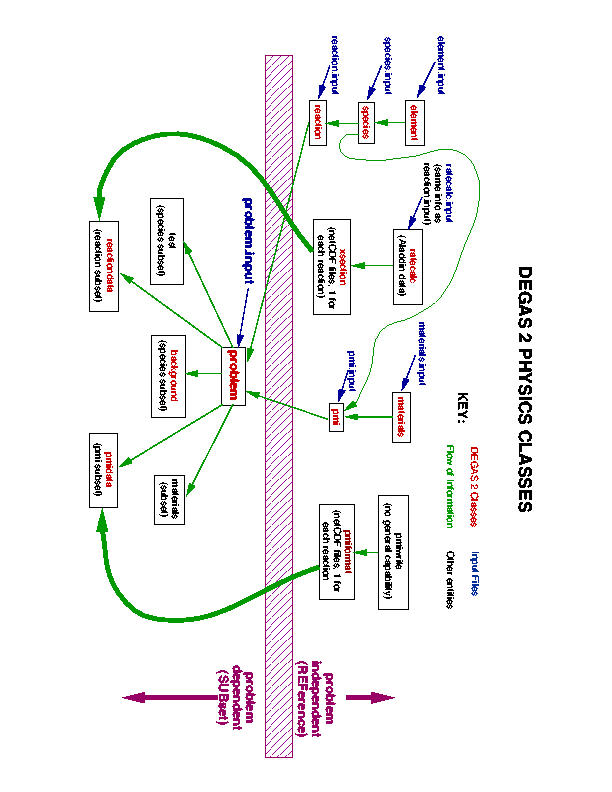
\includegraphics[width=5in,angle=180]{classes_chart}
\caption{Flow of atomic and surface physics data through various DEGAS 2
classes during preprocessing.}
\label{classeschart}
\end{center}
\end{figure}

The data format, evaluation routines, and scoring mechanisms are designed so
that specific quantities can be scored just by adding the appropriate
data to the data file and creating a corresponding tally with that
quantity as the dependent variable. 

One aspect unique to the PMI is that specification of the outgoing velocity
distribution necessarily involves a ``fit'' since standard FORTRAN will
not permit a function (in this case, the function which interpolates
the data tables) to return a vector.

\subsection{An Example: Bateman Format Data}

A particularly involved example of a PMI is the specification of
``Bateman format'' data\cite{Heif82,Bate80}. A few uses of this for
reflection processes are currently in the code. A large set of data
for PMI in an improved version of this format will soon be added.

For each incident
energy and polar angle pair, $(E_{\rm in}, \theta_{\rm in})$,  we have a 
conditional distribution for the product atom
\begin{equation}
P_{E_{\rm in},\theta_{\rm in}}(v,\alpha,\phi) v^{2} dv \: \sin \alpha d\alpha \: d \phi,
\end{equation}
where $\alpha$ and $\phi$ are the outgoing polar and azimuthal angles, 
respectively.

This distribution is sampled from three separate 1-D distributions. First,
the outgoing velocity $v_{0}$ is specified by
\begin{equation}
f^{1}_{E_{\rm in},\theta_{\rm in}}(v) = \int \int P_{E_{\rm in},\theta_{\rm in}}(v,\alpha,\phi)
\sin \alpha d\alpha \: d \phi.
\end{equation}

The outgoing polar angle $\alpha_{0}$ obeys the distribution
\begin{equation}
f^{2}_{E_{\rm in},\theta_{\rm in}}(\alpha) = \int
P_{E_{\rm in},\theta_{\rm in}}(v_{0},\alpha,\phi) d \phi.
\end{equation}

And, finally, the outgoing azimuthal angle $\phi_{0}$ is taken from
\begin{equation}
f^{3}_{E_{\rm in},\theta_{\rm in}}(\phi) = 
P_{E_{\rm in},\theta_{\rm in}}(v_{0},\alpha_{0},\phi).
\end{equation} 

The inverse cumulative distribution, $F(\omega) = G^{-1}(\omega)$, with
\begin{equation}
G(x) = \omega = \int\limits^{x}_{0} f(y) \: dy,
\end{equation}
is specified, say, 5 values of $0 < \omega < 1$. For example,
for a normally incident $\theta_{\rm in}) = 0$, 
$(E_{\rm in} = 1$ eV H atom being reflected off
of Fe, the data are

$R_{N}(E_{\rm in},\theta_{\rm in}) = $ 
\begin{verbatim}
  8.27750E-01
\end{verbatim}

$F^{1}(\xi) =$ 
\footnotesize
\begin{verbatim} 
  1.99146E+00  2.25513E+00  2.32691E+00  2.36544E+00  2.40806E+00
\end{verbatim}
\normalsize
Interpolation into this array with a random number $\xi$ yields 
$\sqrt{E_{\rm out}}$, and thus $v_{0}$.

$F^{2}(\eta,\xi) =$
\footnotesize
\begin{verbatim} 
  5.16532E-01  6.99576E-01  8.11503E-01  8.99906E-01  9.67300E-01
  3.70481E-01  6.11799E-01  7.63020E-01  8.72539E-01  9.61285E-01
  3.80010E-01  6.18834E-01  7.63825E-01  8.75375E-01  9.61256E-01
  3.57688E-01  5.95520E-01  7.51752E-01  8.59766E-01  9.57489E-01
  3.48497E-01  5.17881E-01  6.53833E-01  7.79846E-01  9.23956E-01
\end{verbatim}
\normalsize
A 2-D interpolation into this table with the same first random number $\xi$
and a second one $\eta$ gives $\cos \theta_{0}$.

$F^{3}(\zeta,\eta,\xi) =$ 
\footnotesize
\begin{verbatim}
 -9.54674E-01 -5.93616E-01 -4.55439E-03  6.11607E-01  9.54292E-01
 -9.39719E-01 -5.34726E-01  7.70975E-02  5.91124E-01  9.38723E-01
 -9.47749E-01 -5.99118E-01 -5.34413E-03  5.58645E-01  9.59176E-01
 -9.52932E-01 -5.09963E-01  1.11845E-01  6.68895E-01  9.59592E-01
 -9.63812E-01 -6.32861E-01  2.84474E-02  6.49311E-01  9.65024E-01

 -9.49486E-01 -5.27460E-01  4.71202E-02  5.40823E-01  9.43092E-01
 -9.18789E-01 -5.34890E-01  3.87104E-03  5.97719E-01  9.43635E-01
 -9.35546E-01 -5.66353E-01 -6.17420E-02  5.65376E-01  9.28863E-01
 -9.39133E-01 -5.88361E-01  4.03247E-02  5.36441E-01  9.41553E-01
 -9.42917E-01 -5.66390E-01  4.88304E-03  5.72368E-01  9.58254E-01

 -9.59566E-01 -6.35221E-01 -7.50576E-02  5.72627E-01  9.59374E-01
 -9.43053E-01 -6.23133E-01 -8.35145E-02  5.13894E-01  9.33565E-01
 -9.42753E-01 -6.40605E-01 -1.50300E-02  5.51493E-01  9.32335E-01
 -9.28625E-01 -5.03451E-01  3.69856E-02  6.04412E-01  9.51354E-01
 -9.47567E-01 -5.75171E-01  6.78900E-02  6.17675E-01  9.61149E-01

 -9.42125E-01 -6.25972E-01 -6.74072E-02  5.10579E-01  9.26111E-01
 -9.24288E-01 -5.62514E-01 -6.67559E-02  5.49679E-01  9.57450E-01
 -9.45958E-01 -5.88903E-01  6.07203E-02  5.98492E-01  9.45981E-01
 -9.64714E-01 -6.17340E-01 -2.49212E-02  5.61052E-01  9.49261E-01
 -9.59291E-01 -6.47473E-01 -8.40439E-02  4.58677E-01  9.33637E-01

 -9.43142E-01 -5.25077E-01  4.79891E-02  6.22436E-01  9.53027E-01
 -9.43214E-01 -5.90395E-01  2.32011E-02  5.42675E-01  9.35411E-01
 -9.40994E-01 -4.99927E-01  7.81558E-02  6.19613E-01  9.44418E-01
 -9.35018E-01 -5.38589E-01  8.60652E-02  6.47157E-01  9.51505E-01
 -9.49873E-01 -5.38587E-01  8.93784E-02  6.39298E-01  9.66431E-01
\end{verbatim}
\normalsize
A third random number $\zeta$ is used with the other two in a 3-D
interpolation of this table to obtain $\cos \phi_{0}$. The re-use of
these random numbers in interpolating these three separate dependent
variables means that DEGAS 2 has to treat the random numbers as
fixed independent variables, just like electron density or
ion temperature, rather than generating the random numbers on the
fly in the interpolation process. Hence, the appearance of 
\verb+1st_random_number+, \verb+2nd_random_number+, and
\verb+3rd_random_number+ in the independent variables list
(see the \href{classes.pdf#page.72}{PMI format class}).

So, each file for such PMI contains
\begin{enumerate}
  \item $R_{N}(E_{\rm in},\theta_{\rm in})$,
  \item $F^{1}(\xi,E_{\rm in},\theta_{\rm in})$,
  \item $F^{2}(\eta,\xi,E_{\rm in},\theta_{\rm in})$,
  \item $F^{3}(\zeta,\eta,\xi,E_{\rm in},\theta_{\rm in})$.
\end{enumerate}
Again, all of the data values are stored in a single 1-D array
with the array behavior specified by macros
(see the \href{classes.pdf#page.72}{PMI format class}).

\subsection{Reaction Processing Routines}
\label{reactionprocessing}

Need to create ``set products'' and ``products'' routines, as well as
collision and track-length routines if new type.

\section{Defining Radiation Detectors}

The user defines ``groups'' of detector ``views''. Each view needs
to be defined only once and can be used in more than one group. A
view is defined by:
\begin{enumerate}
  \item Two points,
  \begin{itemize}
    \item The first is taken as the starting point,
    \item The second fixes direction. 
  \end{itemize}
  \item Angular halfwidth (i.e., each view consists of a cone with apex at
the starting point),
  \item An averaging algorithm, used to simulate 3-D behavior with
a cone defined in 2-D (see below). The two techniques available now are
  \begin{itemize}
    \item Uniform weighting,
    \item Circular weighting.
  \end{itemize}
  \item A binning variable,
  \begin{itemize}
    \item Only examples are ``none'' and ``wavelength,''
    \item To use ``wavelength'', would also need to specify a 
minimum, maximum, and the number of wavelength bins.
  \end{itemize}
\end{enumerate}
The actual variables are defined and described in the
\href{classes.pdf#page.42}{detector class}.

Views are machine specific and not frequently changed. For these reasons,
the user will need to specify them via specific lines of code in
{\tt readgeometry} or {\tt boxgen} (both have working examples).

\subsection{Signal Computation}

The contribution from each zone to a view is precomputed so that the
signal can be quickly determined
during or after the run from volumetric emission. 

The 2-D viewing cone is divided into 30 subchords / degree. The code
expects, but does not insist (a warning will be printed), 
that the apex of the cone does not
fall inside a plasma or vacuum zone. Each subchord is tracked from the
apex to the start of a plasma or vacuum zone. From there, the distance
the subchord traverses through each zone is computed. The subchord is
terminated when it reaches a solid zone; this is the actual end point.
The resulting contribution made to the view by zone $j$, call it $f(z_{j})$,
is for $i = 2N+1$
uniformly weighted subchords
\begin{equation}
f(z_{j}) = \sum_{i=-N}^{N}  d_{i,j} w_{i} / V_{j},
\end{equation}
where $d_{i,j} = $ is the distance along subchord $i$ through zone $j$, 
and $V_{j}$ is the volume of zone $j$.  The relative weight of each
subchord is $w_{i}$ with
\begin{equation}
w_{i}^{\rm uniform} = \frac{1}{4 \pi (2N + 1)},
\end{equation}
and
\begin{equation}
w_{i}^{\rm circular} = \frac{1}{2 \pi^{2} N \sqrt{1 - (i/N)^2}}.
\end{equation}
The units of $f$ are ${\rm m}^{-2}/{\rm st}$.

These zone contributions can then be used during execution of the main
code or during post-processing to compute, say, the 
H$_{\alpha}$ signal $S_{\alpha}$
in the absence of recombination  (see Sec.~\ref{AtomicPhysics}) as
\begin{equation}
S_{\alpha} = \sum_{j} N_{1}(z_{j}) \left[ \frac{N_{3}}{N_{1}} 
A_{23} E_{23} \right] f(z_{j}),
\end{equation}
where $N_{1}$ is the number of neutral H atoms in zone $j$. The
bracketed quantity is interpolated from the input data file, with $E_{23}$
being the energy of the Balmer-$\alpha$ transition, and other quantities
defined in Sec.~\ref{AtomicPhysics}.
Note, however, that the code is completely general regarding wavelength 
and origin of radiation. Other line emission rates can be scored in
an analogous if the appropriate data are present in the input data
files. Again note that the views cannot be toroidally directed. If
needed, this option could be incorporated with relative ease.

\section{Sectors and Diagnostic Surfaces}

The default behavior for a surface in DEGAS 2's tracking algorithm is
to stop the flight momentarily (to check for a zone boundary) and then
to continue. In some instances, these surfaces need to do more, e.g.,
\begin{enumerate}
  \item If that surface represents the interface between a plasma or
vacuum zone and a material (solid) or exit zone, the quantities describing
the flight must be altered to represent the effect of that next zone,
  \item If the user wishes to monitor the passing of a flight through a
particular surface, the flight's parameters must be noted and used to
update the appropriate tallies.
\end{enumerate}

To address these needs, DEGAS 2 utilizes the {\em sector} concept.
The most general description of a sector is a coupled surface and 
a zone. More specifically, the surface should be a bounding surface
of a cell comprising the zone (the orientation is important; see below).
The function used to define sectors takes as an optional argument a
second zone. If provided, the function will verify that the input surface
is indeed an interface between the two zones. The programmer should use
this option whenever possible as a consistency check. 

Solid zones in DEGAS 2 are typically physically larger entities than
plasma zones. E.g., many plasma zones may be in contact with the same
solid zone. Although this approach simplifies specification of the
geometry, it prevents local variations in the properties of the solid
zone, such as material temperature or recycling coefficient. Instead,
we will use the sectors to store data such as these. In contrast,
each plasma zone has associated with it local data, such as plasma 
temperature and density. By including the plasma zone number in the
sector definition, the sectors have access to the properties of both the
material and plasma at the interface between the two. The particular
properties required may vary with the model used process the flights
as they strike the interface. The existing geometry setup routines
({\tt readgeometry} and {\tt boxgen}) define take care of the definition of
these sectors. In the case of {\tt readgeometry}, little or no input is
required from the user. 

Sectors can also be defined for purely diagnostic use. The zones adjacent
to the sector surface can be of any type. A given sector may be used to
specify more than one diagnostic (e.g., one may track particle current,
another might tally particle energy).

Because of the inherent differences between interfaces of different types,
the sectors must be categorized into subclasses:
\begin{description}
  \item[target] The interface between a plasma zone and a solid zone,
  \item[wall] The interface between a vacuum zone and a solid zone,
  \item[exit] The interface between a vacuum or plasma zone and an
exit zone,
  \item[diagnostic] A diagnostic sector.
  \item[plasma] A sector type used in an earlier version of the code,
retained only for backward compatibility. 
  \item[vacuum] A sector type used in an earlier version of the code,
retained only for backward compatibility. 
\end{description}

To facilitate output organization, sectors have labels associated with them,
{\tt strata} (for groups of sectors) and {\tt sector\_strata\_segment}
(for an individual segment). The user can specify these in an arbitrary 
manner. {\tt readgeometry} provides some keywords for this purpose.

Additional details on the sector subclass properties can be found
in the documentation on the \href{classes.pdf#page.34}{sector class}.

\subsection{Diagnostic Sectors}

Diagnostic sectors are defined in a manner closely paralleling that of 
detectors. Diagnostic sector groups are used to identify sectors of
similar functionality. Both {\tt readgeometry} and {\tt boxgen} define
default diagnostic groups using the non-diagnostic sectors set up 
by those routines:
\begin{description}
  \item[Wall and Target Counts] Includes all wall and target sectors. No
independent variable is associated with this diagnostic group; it is only
capable of summing a particular test particle property (which will be
specified by a corresponding tally, particle mass, for example).
  \item[Exit Counts] Includes all exit sectors. No
independent variable is associated with this diagnostic group either.
  \item[Wall and Target Energy Spectrum] Specifies the particle
energy as the independent variable. As in the ``Counts'' groups, some
as-yet-unspecified particle property will be tracked. The difference is
that the tally will be divided up into the energy bins defined for this
group.
  \item[Wall and Target Angle Spectrum] Similar to the ``Energy Spectrum''
group, but the independent variable is the angle of incidence of the particle.
\end{description}

In addition, the definition of dioagnostic only sectors and a corresponding
group (``Throat sectors'') is illustrated in {\tt readgeometry.web}.

The particle properties to be associated with these diagnostic
groups for the purpose of defining tallies may be directionally
dependent. For instance, the particle current leaving and entering
a zone may be specified separately. Details will be given in 
Sec.~\ref{tallies}.

\section{Estimators and Specification of Tallies}
\label{tallies}

\begin{itemize}
  \item Introduce first two types of $g$'s: ``test particle'' and 
``reaction'',
  \item Corresponding DEGAS 2 estimators:
  \begin{enumerate}
    \item $\eta_{g}^{\rm TLE} = w \, \frac{1 - \exp(-\sigma_{i} t_{V})}{\sigma_{i}} g$,
    \begin{itemize}
      \item {\bf Track Length Estimator,}
      \item $t_{V} =$ time track spent in volume V,
      \item $w =$ weight at start of time step.
      \item $g$ can be a test particle attribute: 
mass, momentum, energy,
      \item or reaction-related, e.g., ion 
momentum source due to charge exchange,
      \item Latter $g$'s enter TLE as averages over background 
distribution [Reiter, 1993].
    \end{itemize}
    \item $\eta_{g}^{\rm CE} = \sum_{m_{s}} w_{m_{s}} \frac{g}{\sigma_{s}}$,
    \begin{itemize}
      \item {\bf Collision Estimator,}
      \item Summed over $m_{s}$ all scattering collisions within $V$,
      \item $w_{m_{s}} = $ weight at $m_{s}$th collision,
      \item $g$ is test particle attribute.
    \end{itemize}
    \item $\eta_{g}^{\rm CE} = \sum_{m_{j}} w_{m_{j}} \frac{g}{\sigma_{j}}$,

    \begin{itemize}
      \item {\bf Collision Estimator for Reaction $j$,}
      \item Summed over $m_{j}$ collisions of reaction $j$ within $V$,
      \item $g$ is reaction-related, 
      \begin{itemize}
        \item Likely something known only at collisions,
        \item E.g., energy source due to H$_{2}$ dissociation.

      \end{itemize}
    \end{itemize}
    \item Many integrals of interest can be written as:
\[
I(g) \equiv \int d^{3}r g(\vec{r}) \int d^{3}v f(\vec{r},\vec{v}) = 
\int d^{3} r g(\vec{r}) n(\vec{r}),
\]
    \begin{itemize}
      \item {\bf Post-Process Estimator,}
      \item For $g$'s not dependent upon test or background velocities,
      \item E.g., H$_{\alpha}$ emission rate.
    \end{itemize}
  \end{enumerate}
  \item Third type of score is diagnostic sector  (surface),
  \begin{itemize}
    \item Estimator is just $w g$,
    \item $w =$ weight when track hits sector,
    \item $g =$ mass, incident angle, or energy,
    \item Labeled as a {\bf collision estimator}
  \end{itemize}
  \item In summary, DEGAS 2 has:
  \begin{itemize}
    \item Three types of scores or ``tallies'' according to nature of $g$
    \begin{enumerate}
      \item Test,
      \item Reaction,
      \item Sector.
    \end{enumerate}
    \item Three estimators:
    \begin{enumerate}
      \item Track Length,
      \item Collision,
      \item Post Process.
    \end{enumerate}
  \end{itemize}
\end{itemize}


\begin{itemize}
  \item Specify for each tally:
  \begin{enumerate}
    \item Descriptive label,
    \item Type for $g$,
    \item Geometry,
    \begin{itemize}
      \item Volume (per zone),
      \item Surface (diagnostic sector),
      \item detector (chord-integrated).
    \end{itemize}
    \item Dependent variable, e.g.,
    \begin{itemize}
      \item Energy,
      \item Background momentum,
      \item H$_{\alpha}$ emission rate.
      \item Matched directly against labels in atomic physics data files \\
$\Rightarrow$ easily score new variables.
    \end{itemize}
    \item Rank,
    \item Independent variables (1 $\rightarrow$ Rank), e.g.,
    \begin{itemize}
      \item Zone,
      \item Test particle species,
      \item Energy bin (diagnostic sector),
      \item Wavelength bin (detector).
    \end{itemize}
    \item Estimator,
    \begin{itemize}
      \item For reaction types, may vary with reaction.
      \item May be advantageous to combine results from than one estimator, but
not implemented now.
    \end{itemize}
    \item {Conversions} to be performed on tally,
    \begin{itemize}
      \item Usually to do some {scaling prior to output}, e.g., by
      \begin{itemize}
        \item mass,
        \item volume.
      \end{itemize}
      \item {Important example: converting $\vec{v}$ from Cartesian
to cylindrical coordinates when scoring.}
    \end{itemize}
  \end{enumerate}
\end{itemize}

\newpage

\section*{ \protect \Huge{\bf {OUTPUT FORMAT}}}

\begin{itemize}
  \item {On output, tally data appear in four arrays:}
  \begin{enumerate}
    \item Sorted by neutral sources, prior to post-processing,
    \item Summed over neutral sources, prior to post-processing,
    \begin{itemize}
      \item Only these have standard deviation data.
    \end{itemize}
    \item Sorted by neutral sources, after post-processing,
    \item Summed over neutral sources, after post-processing.
  \end{enumerate}
  \item {Separate output array for data to be passed to
2-D fluid plasma code.}
  \item {All output data written to a netCDF file.}
  \item Example text output data are written by main code.
  \item {A separate code which reads output netCDF file \\ and generates 
HDF data and images provided as an example.}
\end{itemize}


\chapter{Other Documentation}
\label{otherdoc}

(Provide links to significant inline documentation sections; e.g.,)

\section{Random Numbers}
\label{randomnumbers}

The concepts behind the random number generator used in DEGAS 2 are
described in the file {\tt random.web}. The 
\href{random.pdf#page.1}{documentation} at the top of the file
provides a nice introduction.

\section{Atomic Physics Rate Calculation}

The {\tt ratecalc} code is used to compute atomic physics reaction
rates from cross section data, as well as a few other tasks. 
The code is documented internally. Follow this
% To get this to work, had to add some stuff to fweb.sty (the hyperref
% package). Can then do: pdflatex ratecalc.tex. 
% Note that this page
% number is the one TeX assigns; not the one acroread uses.
% pdflatex will complain occasionally about ``non-pdf special'', but
% I don't see any deleterious effects so far (appears to have something
% to do with section headers).
\href{ratecalc.pdf#page.1}{link} to
the introductory section to learn more.

\section{Code Variables}

The file {\tt classes.web} contains an extensive description of what
the code looks like internally. Most of the common variables (i.e.,
the contents of the {\tt hweb} header files) are documented here
as well. Try following this 
\href{classes.pdf#page.1}{link} if
you want to have a look at it now.

\section{Geometry Details}

The introduction to {\tt geometry.web} provides a concise description
of the fundamental elements of the DEGAS 2 geometry. Here's a 
\href{geometry.pdf#page.1}{link} to the PDF version of this file.
Note that most users will define geometries at a higher level,
such as that provided by {\tt readgeometry} and {\tt boxgen}. 

\chapter{EIRENE Benchmark}

\section{Introduction}

Since UEDGE was first coupled to EIRENE and since EIRENE is currently the most
widely used neutral transport code in the field, the first step in coupling 
DEGAS 2 is to perform a benchmark against EIRENE. A simple slab, 
``single-null'' geometry and plasma generated by UEDGE is used as input
to both codes. An \href{http://w3.pppl.gov/degas2/DE_Bench/}{initial effort}
was performed without recombination. Essential information from that 
documentation has been included here for completeness.

This chapter describes a second round of benchmark exercises in which
recombination is accounted for.
The plasma $T_{e,i} \sim 1$ eV near plate in this case. For reasons 
to be explained below, several numerical differences
between the codes are accentuated under these conditions. We will describe
here the isolation and elimination of most of these differences, enabling
us to get agreement of densities and plasma sources to within $5 \%$.
In the process we have developed a means for quantitatively comparing the
code results. 

% Note: can probably just incorporate useful info from previous
% benchmark: change to energy distribution, basic atomic physics
% comparison (maybe), and performance benchmark.

The following sections will: 
\begin{enumerate}
  \item Describe the geometry, boundary conditions, and UEDGE plasma,
  \item Qualitatively compare ``out of the box'' code results,
  \item Describe how code results are quantitatively compared,
  \item Explain several differences between the codes, eliminating or
minimizing them when possible,
  \item Characterize the level of agreement between the codes,
  \item Go through a performance benchmark and optimization of DEGAS 2.
\end{enumerate}

\section{Problem Description}

The geometry is intended to be a 2-D slab representation of a toroidally
symmetric single-null scrape-off layer. The resulting ``box'' is 1 m
long, extending from a mirror boundary at $Z = 0$ to a molybdenum target
plate at $Z = 1$ m. Only half of the scrape-off layer is being simulated;
hence, the appearance of the mirror. The radial width is 0.05 m.
An exit is used to represent the core boundary at $R = -0.01$ m
between $Z = 0$ and $Z = 0.75$ m. The outer wall at $R = 0.04$ m
is assumed to be made of molybdenum. The section representing the
wall adjacent to the private flux region, at $R = -0.01$ m
between $Z = 0.75$ m and $Z = 1$ m, is also taken to be made of
molybdenum.  Finally, a mirror surface at $Z = 0.75$ m extending from
$R = -0.01$ m to $R = 0$ creates a private flux region above it.
The length of the box in the third dimension is 1 m, although
periodic boundary conditions are established at both ends.

The UEDGE mesh has a nonuniform spacing with 64 zones in the $Z$
direction and 32 in $R$. The geometry and plasma data are provided to
DEGAS 2 in a file generated during UEDGE post-processing by the BASIS 
utility. The electron temperature and density computed by UEDGE
with its fluid neutral transport model are shown in Figs.~\ref{te}
and \ref{ne}.

\begin{figure}
% \epsfverbosetrue
\begin{center}
\leavevmode
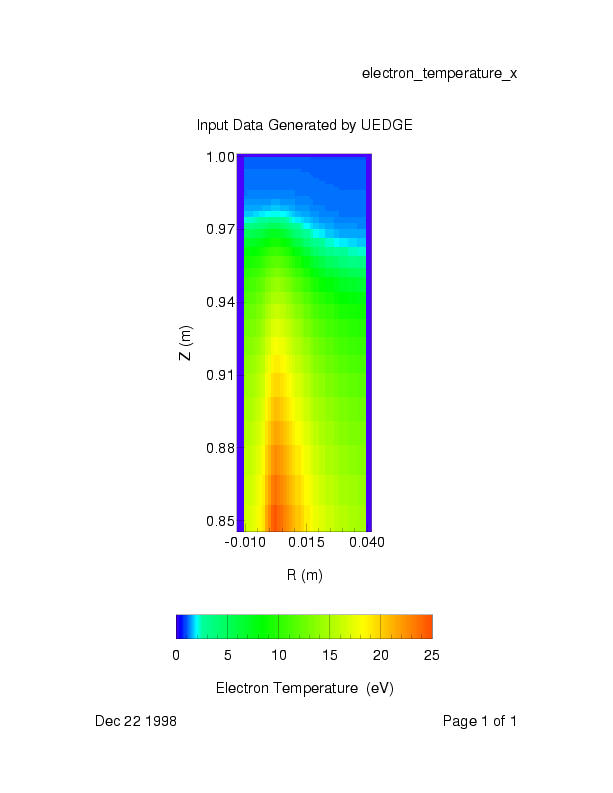
\includegraphics[width=5in]{te}
\caption{Electron temperature near the target ($Z = 1$ m) as computed by 
UEDGE with its fluid neutral model. }
\label{te}
\end{center}
\end{figure}

\begin{figure}
% \epsfverbosetrue
\begin{center}
\leavevmode
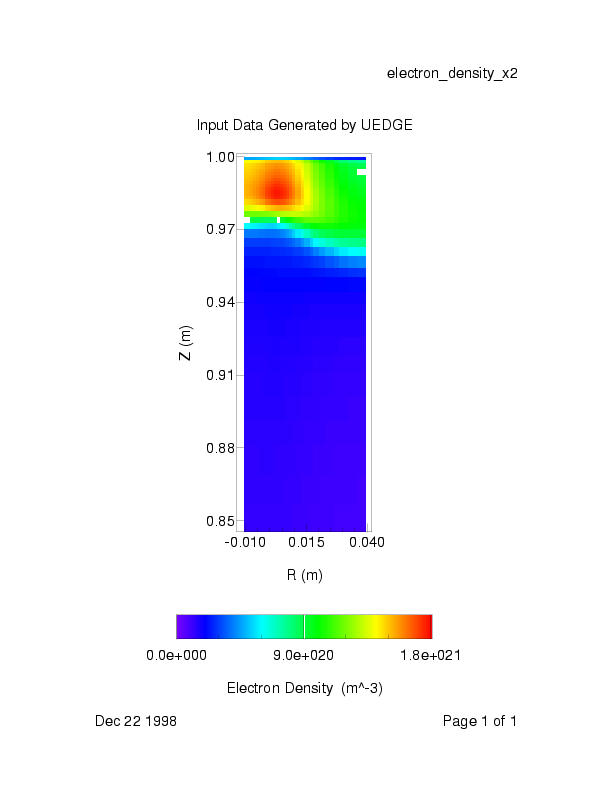
\includegraphics[width=5in]{ne}
\caption{Electron density near the target ($Z = 1$ m) as computed by
UEDGE with its fluid neutral model.}
\label{ne}
\end{center}
\end{figure}

\section{``Out of the Box'' Results}
\label{outofthebox}

Figures~\ref{eirDden} and \ref{degas2Dden} show how the atomic deuterium
densities computed by EIRENE and DEGAS 2 using the UEDGE plasma compare
with roughly standard physics.  The word ``roughly'' is meant to imply
that some of the changes to be described later in this chapter have
been incorporated into these simulations. For EIRENE, the random
number problem (see Sec.~\ref{sampling}) has been remedied. For DEGAS 2,
the treatment of reflection used on the molybdenum surfaces uses
the EIRENE data, including the attempts to mimic EIRENE's extrapolation
behavior (see Secs.~\ref{erefl} and \ref{arefl}).

\begin{figure}
% \epsfverbosetrue
\begin{center}
\leavevmode
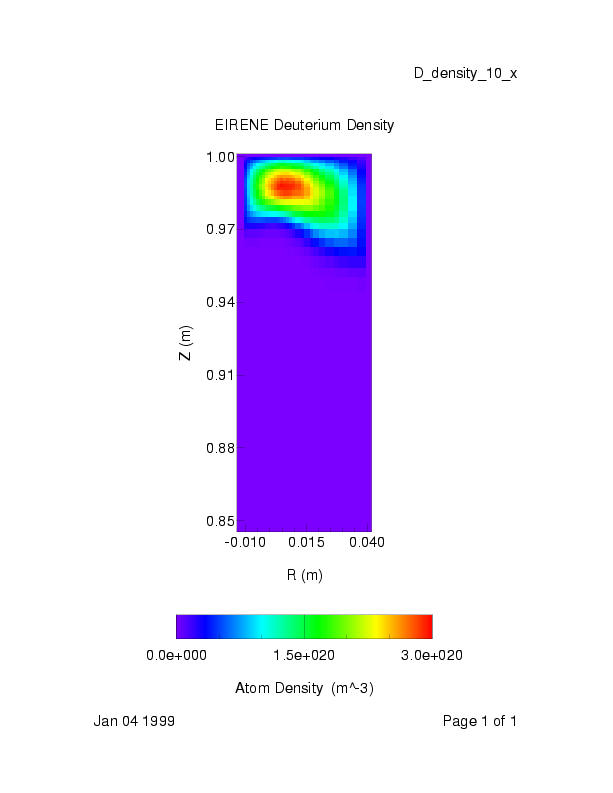
\includegraphics[width=5in]{eir_D_den}
\caption{Neutral deuterium atom density computed by EIRENE.}
\label{eirDden}
\end{center}
\end{figure}

\begin{figure}
% \epsfverbosetrue
\begin{center}
\leavevmode
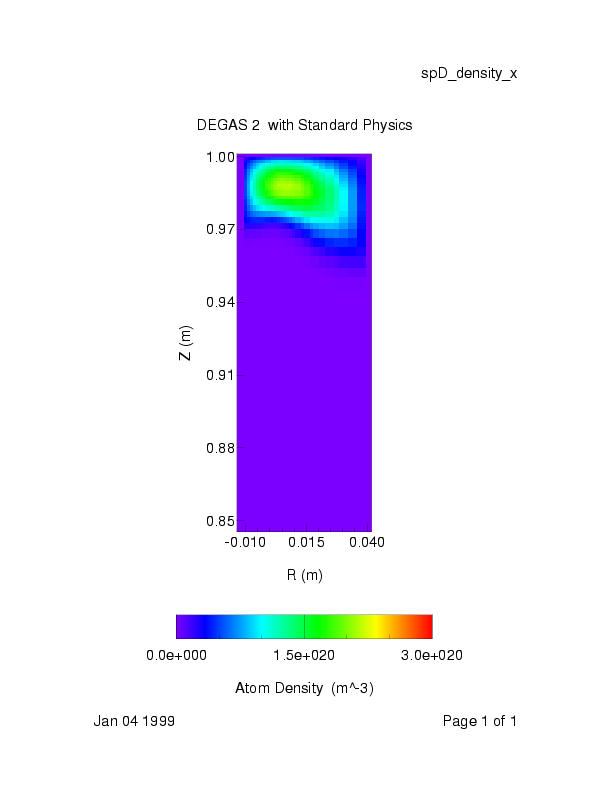
\includegraphics[width=5in]{degas2_D_den}
\caption{Neutral deuterium atom density computed by DEGAS 2 using ``standard
physics''.}
\label{degas2Dden}
\end{center}
\end{figure}

The peak EIRENE density is about $3 \times 10^{20}$ m$^{-3}$. For DEGAS 2,
the peak is only about $2 \times 10^{20}$ m$^{-3}$. In Sec.~\ref{codediffs},
we will list the causes of this discrepancy and describe the techniques
we use to eliminate or minimize them.

\section{Statistical Basis for Comparisons}
\label{statcompare}

Because Monte Carlo codes provide only a statistical description of
a result, e.g., the neutral density at a particular point in space 
and an estimate of its error, comparisons between codes require some
care. Differences between codes smaller than the standard error in their
results cannot be discerned, as this section will demonstrate. 
We will describe a quantitative procedure for comparing code results
which can be used to tell if the differences cannot be statistical
in nature.

The
standard error decreases with $1/\sqrt{N}$, where $N$ is the number
of flights, and can in principle be made as small as desired. For the
problem at hand, we've used 80,000 flights for each of the source
groups, resulting in standard errors of a few percent near the plate
for simple tallies such as the neutral atom density. The differences
between EIRENE and DEGAS 2 remaining after the steps described in 
Sec.~\ref{codediffs} have been taken are slightly larger than this, so
raising the number of flights further would not be useful.

Both DEGAS 2 and EIRENE compute the recombination  contributions to
the source terms (e.g., subtracting recombination rate from the ion
particle source) directly and add them to the final Monte Carlo results
at the end of the run. DEGAS 2 does provide the option for computing
these contributions in the standard Monte Carlo way (as a check), but
the statistical error is increased substantially.
Comparison of the code results is, thus, further complicated because the
computed variance estimates cannot be used directly with the final output
results.
Rather, our statistical comparisons must be made {\em without} these
``post-processing'' contributions.

DEGAS 2 has two sets of output arrays:
\begin{enumerate}
   \item One written before post-processing and containing relative
standard deviations,
   \item One with the post-processing results and no variance data.
\end{enumerate}
The screen output generated by EIRENE likewise contains 
results without these post-processing
contributions and their relative standard deviations, provided
they were requested in the input file. These data along with the
first of the two DEGAS 2 output array sets will be analyzed with
the procedure outlined here.  

The principal basis our statistical comparison is the Central Limit 
Theorem\cite{Span69}. Say we have the density score in a particular zone 
from a run of
$K$ flights; call it $\mu_{K}$. This result is effectively a sample 
drawn from a parent population; call its mean $m$ and the 
standard deviation $\sigma$. The objective of the Monte Carlo method is 
to estimate this mean $m$.

The Central Limit Theorem then says that the relative error
\begin{equation}
\epsilon_{\rm rel} \equiv \frac{ | \mu_{K} - m | }{ \sigma_{K} },
\end{equation}
where $\sigma_{K} = \sigma / \sqrt{K}$ is the standard error,
has a Maxwellian distribution.
That is, the probability that $\epsilon_{\rm rel} < 1$ is 
$68.3 \%$, $< 2$ is $95.4 \%$ and $< 3$ is $99.7 \%$.

To apply this directlyto our situation, we would need to:
\begin{itemize}
  \item Do many runs of both codes, 
  \item Find values of $m$ for each code which are consistent with
those results,
  \item Compare the $m$ values between codes,
  \item Repeat the process for each zone.
\end{itemize}
 
Such a process is too lengthy to permit extensive comparisons
of different variables and input conditions. We propose using
instead a simpler, compromise procedure.
Say we have a density score from DEGAS 2 $\mu^{\rm D}_{K}$ and
one from EIRENE $\mu^{\rm E}_{K^{\prime}}$,
We begin by {\em postulating} that they have the same $m$,
If this is true, the random variable $z \equiv \mu^{\rm D}_{K}
- \mu^{\rm E}_{K^{\prime}}$ has mean $m_{z} = 0$,
Then, if each of the codes' standard deviation estimates
$s^{\rm D}_{K}$ and $s^{\rm E}_{K^{\prime}}$ are also consistent with
$\sigma$, one can show that the distribution of $z$ about its
mean $0$ will have a standard deviation
\begin{equation}
s_{z,K,{\rm eff}} = \sqrt{(s^{\rm D}_{K})^{2} 
+ (s^{\rm E}_{K^{\prime}})^{2}},
\end{equation}
This is just what one expects from propagation of errors.

We are not done yet in that applying this would still require
many runs of both codes.
However, we do have many zones in each run.
{\em If} the scores in each zone are uncorrelated with other
zones, we could treat the value of 
\begin{equation}
\epsilon_{z,{\rm rel}} = 
z / s_{z,K,{\rm eff}}
\label{epsilonrel}
\end{equation}
in each
zone as a separate sample and compile a distribution of 
$\epsilon_{z,{\rm rel}}$ by comparing the results in each zone.
If we find this distribution to be Maxwellian, we may infer that our 
postulates are correct, i.e., the codes are giving the same results.
If the distribution strongly deviates from a Maxwellian, we can suspect
that the codes do not agree.

The extent to which scores in two zones are correlated depends
on many factors. Since we do not require precise statistical agreement
between the codes (a few percent of systematic error is acceptable), we
will assume that the effect of these correlations is too small to prevent this
test from detecting significant (more than a few percent) differences.

One other consideration is that the Central Limit Theorem only
applies for ``large enough $K$''.
For a given zone, this effectively means a ``small enough
relative standard deviation''.
For these comparisons, both codes produce relative standard
deviations near the target of a few percent.
If we restrict the comparison to zones with relative standard
deviations below some value, say $\sigma_{\rm max} = 20 \%$, 
we should still have a large
number of zones to work with.

Note that the codes output the relative standard deviation,
$\sigma / (m \sqrt{K})$.
To get $\sigma^{\rm D}_{K}$ we multiply the 
output relative standard deviation by $\mu^{\rm D}_{K}$.

\section{Code Differences}
\label{codediffs}

\subsection{Atomic Physics}

The common ancestry of EIRENE, DEGAS, and DEGAS 2 is apparent in their
atomic physics data. All three
codes rely upon the molecular data in the Janev book\cite{Jane87} (see 
Sec.~\ref{h2rate}, however). The reaction rates
are explicitly the same in all three codes, as are the dissociation energies,
and the electron energy loss rates. 
Note also that since the 
scoring of momentum transfer to the plasma in EIRENE is relatively new, 
its implementation is incomplete: there is no momentum transfer for the
molecular dissociation processes. However, given the dominance of the other
momentum sources, this should not be a problem. DEGAS 2 tracks all three
components of the momentum transfer in all reactions.

This version of EIRENE (with the present input file) uses the reaction
rate for charge exchange in the Janev book\cite{Jane87}. 
No attempt is made to ensure
that the sampled background ion velocities are consistent with the 
charge exchange cross section\cite{Heif82}.
Furthermore, the momentum and energy transfer expressions are correct only
in the limit of $\langle \sigma v \rangle = \sigma v$ 
(see Sec.~\ref{estdiffs}). More recent
versions of the code certainly do better than this\cite{Reit93}.

The DEGAS 2 standard charge exchange data comes from
the
Janev-Smith database\cite{Jane93}, with 
consistently computed reaction rates, and
energy and momentum transfer rates\cite{Reit93}. The simulation described in
Sec.~\ref{outofthebox} used these data. For subsequent runs, data
equivalent to those in EIRENE will be substituted.

DEGAS 2 and EIRENE each rely on their own collisional 
radiative\cite{Reit93} codes for 
the multi-step electron-impact ionization and recombination of 
hydrogen data. 
These two codes have been compared several times in the past.
The basic
difference is that the EIRENE code, AMJUEL, 
is based upon the Johnson-Hinnov ionization cross sections\cite{John73}.
The data used in DEGAS 2 are described in Sec.~\ref{AtomicPhysics}.

Figures~\ref{hionize} and \ref{eloss}
compare the rate data. The AMJUEL ionization rates are noticeably lower
for $T_{e} < 10$ eV. This is likely responsible for most of the
differences between the densities in Figs.~\ref{eirDden} and 
\ref{degas2Dden}. The energy loss rates agree. However, when normalized
to the ionization rate, to give the energy lost per ionization, the
differences of Fig.~\ref{hionize} are factored in. 

\begin{figure}
% \epsfverbosetrue
\begin{center}
\leavevmode
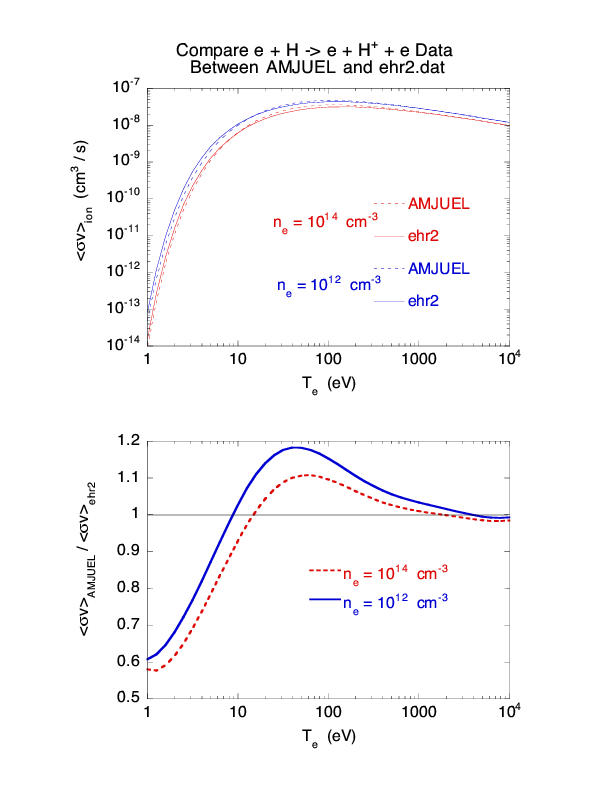
\includegraphics[width=5in]{Hionize_Comparison}
\caption{Comparison of effective collisional radiative electron impact
hydrogen ionization rate from EIRENE's
AMJUEL data file and from DEGAS 2's IRLS code (contained in the
publicly distributed file {\tt ehr2.dat}) at
densities of $10^{18}$ m$^{-3}$ and $10^{20}$ m$^{-3}$. The lower
figure shows the ratios of the rates computed by the two codes.}
\label{hionize}
\end{center}
\end{figure}

\begin{figure}
% \epsfverbosetrue
\begin{center}
\leavevmode
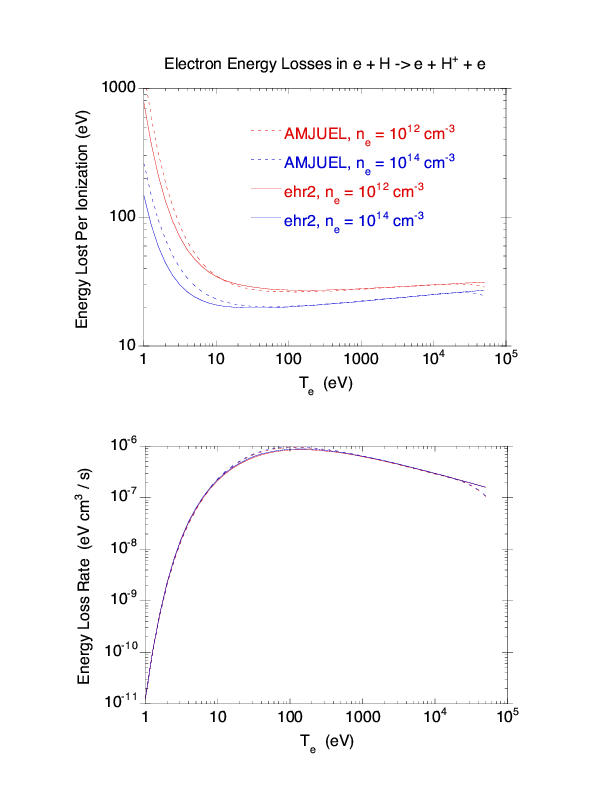
\includegraphics[width=5in]{E_Loss_Comparison}
\caption{Comparison of effective collisional radiative electron energy
loss rate from EIRENE's
AMJUEL data file and from DEGAS 2's IRLS code (contained in the
publicly distributed file {\tt ehr2.dat}) at
densities of $10^{18}$ m$^{-3}$ and $10^{20}$ m$^{-3}$. The upper figure
shows the energy lost per ionization; the lower gives the power
lost.}
\label{eloss}
\end{center}
\end{figure}

Figure~\ref{hrecombine} shows that the recombination rates agree well. 
The reason is that the Johnson-Hinnov\cite{John73} 
recombination cross section data are used in both collisional radiative
codes. The energy exchange rates agree for $T_{e} < 10$ eV, but disagree
at higher temperatures. This quantity includes the average energy of
a radiatively recombining electron; the expression used to compute 
it involves\cite{Reit93} 
$d \langle \sigma v \rangle_{\rm recombination} / d T_{e}$. Apparently,
the AMJUEL values were obtained by differentiating a fit to
$\langle \sigma v \rangle_{\rm recombination}$. The values used in DEGAS 2,
however, were obtained by differentiating closed form expressions for
$\langle \sigma v \rangle_{\rm recombination}$ and should be correct.

\begin{figure}
% \epsfverbosetrue
\begin{center}
\leavevmode
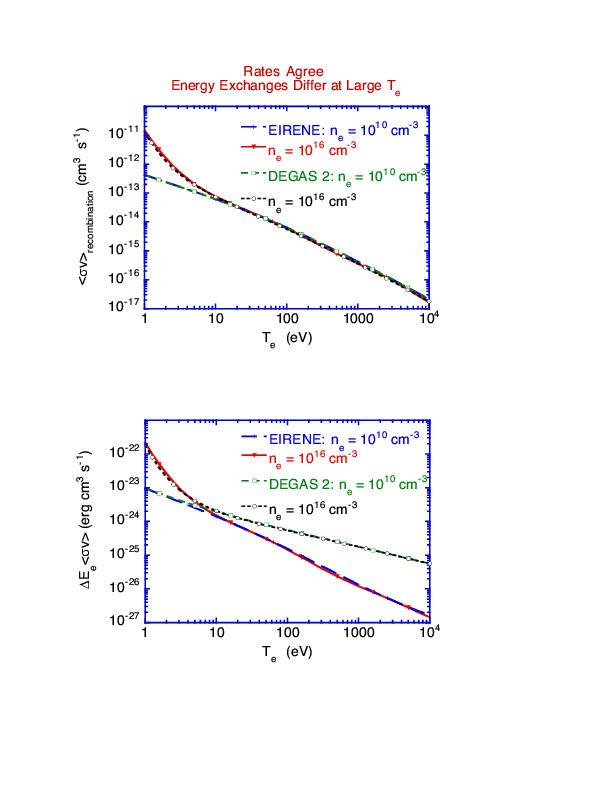
\includegraphics[width=5in]{Recomb_Plots}
\caption{Comparison of effective collisional radiative electron recombination
rates from EIRENE's
AMJUEL data file and from DEGAS 2's IRLS code (contained in the
publicly distributed file {\tt ehr2.dat}) at
densities of $10^{16}$ m$^{-3}$ and $10^{22}$ m$^{-3}$. The upper figure
shows the effective recombination rates; the lower gives the power
lost.}
\label{hrecombine}
\end{center}
\end{figure}

As with charge exchange,
in Sec.~\ref{outofthebox} DEGAS 2 used the {\tt ehr2.dat} data. 
For subsequent runs, the AMJUEL data will be used in both codes.

\subsection{Source Sampling}
\label{sampling}

The ion current distribution to the target is sampled according to
the relative fractions of current striking each segment (i.e., each
radial zone). Likewise, the probability distribution used in sampling
the ``birth'' zone of a recombining ion is given by the fraction of the
total recombination occurring in that zone. Whether or not a code is
correctly sampling these distributions can be easily determined. For
DEGAS 2, the {\tt sourcetest} utility was written to do just this
(see Sec.~\ref{testroutines}). Cruder means were used to extract the
requisite data from EIRENE.

Figure~\ref{sourcesegments} shows that the two codes are able to match
the input distribution (to within the error bars). To make the comparison
quantitative, we use a $\chi^{2}$ test\cite{Bevi69}. The result is $p$, 
the probability that sampled distribution  matches the parent distribution.
For the 5000 samples used in generating Fig.~\ref{sourcesegments}, 
the DEGAS 2 results yield $p = 0.97$. For EIRENE, we get $p = 0.69$. 
Since $p$ in both cases is not too much smaller than 1, we conclude that
the input distribution is being adequately sampled.

\begin{figure}
% \epsfverbosetrue
\begin{center}
\leavevmode
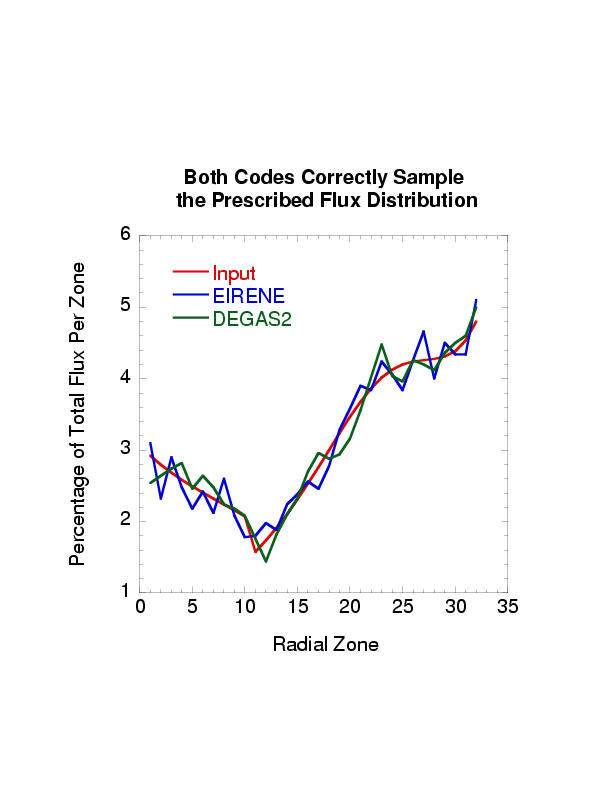
\includegraphics[width=4in]{source_segments}
\caption{Sampled target flux distributions, as a function of radial zone,
for DEGAS 2 and EIRENE. The curve labeled ``Input'' is the ideal
result.}
\label{sourcesegments}
\end{center}
\end{figure}

We use 50,000 samples of the recombination source. Because of the
large number of zones, a simple plot analogous to Fig.~\ref{sourcesegments}
is unintelligible. Furthermore, not all of the problem zones are 
adequately sampled to permit the application of a $\chi^{2}$ test to the
whole problem space. Instead, we isolate the 648 zones 
with highest recombination rate (the lowest
temperature region, chosen somewhat arbitrarily). Applying a
$\chi^{2}$ test to samples taken in those zones yields for
DEGAS 2 $p = 0.94$. But, for EIRENE $p = 0.21$. Sensing that this is
small enough to cause concern, we repaired a known problem with the
EIRENE random number generator (as received, the code had random number
seeds which differed by unity; the fix is to make one of these integers
very different). The result is much improved: $p = 0.79$. All other
EIRENE runs described in this chapter utilize this bug fix.

\subsection{Energy Distribution of Reflected Atoms}
\label{erefl}

The EIRENE surface physics is more detailed than 
that of the old DEGAS and, hence, DEGAS 2. Consequently, we will
not make an overall comparison with different
surface physics data. Instead, we have translated the Bateman format data 
for reflection of D off of Mo taken from EIRENE's {\tt TRIM} input
file into a DEGAS 2 format. To be more precise, the Mo data obtained from
Fe data using a scaling argument\cite{Ecks91}.

These data prescribe the reflection coefficient, the outgoing energy, and
two outgoing angles as a function of the incident energy and polar angle.
The Bateman format is described in detail elsewhere\cite{Heif82}.
Briefly, these data specify these parameter values (e.g.,
the outgoing energy) at
intervals of the cumulative distribution function: 0.1, 0.3, 0.5, 0.7, 0.9.
One can also establish data points at each end of the distribution. 
For example,
a minimum energy might be the wall temperature; a maximum would be the
incident energy. As originally implemented in DEGAS 2, this 
additional information to
extrapolate beyond the ends of the data. Doing this carefully required
specifying additional cumulative distribution values at 0, 0.2, 0.4, 0.6,
0.8, and 1.0 (intermediate values being obtained by linear interpolation).

EIRENE, however, mindlessly extrapolates the data and enforces the minimum
and maximum values after sampling. The result is that the sampled maximum
and minimum may be noticeably different from what one expects.
The \href{http://w3.pppl.gov/~dstotler/DE_Bench/full_code.html}{first set of benchmark runs}
indicated that the difference in the
handling of the lowest reflected energy atoms was significant. The
reason is that the atom density near the target plate (i.e., where
ionization is lowest) scales like the inverse of the atom velocity,
and hence is impacted strongly by the lowest energy atoms. To 
eliminate this difference, we reset the lower bound on the energy 
so DEGAS 2 would mimic the EIRENE extrapolation. Figure~\ref{edistrevised}
shows that the original DEGAS 2  reflected energies for a normally 
incident 19 eV atom match the input data well
(the difference at the lower end is due to the use of logarithmic 
interpolation in DEGAS 2). The revised DEGAS 2 reflected energies differ
from the input, but better match the values obtained from EIRENE.

\begin{figure}
\begin{center}
\leavevmode
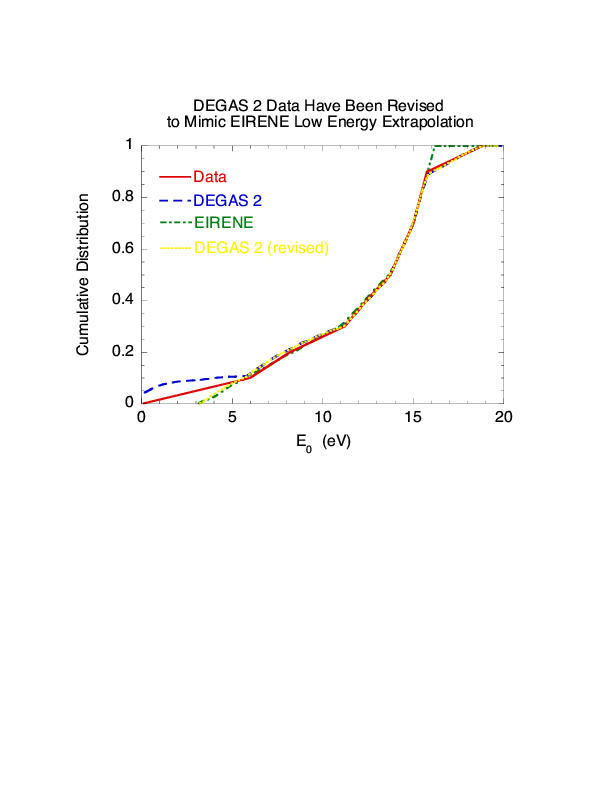
\includegraphics[width=5in]{E_dist_revised}
\caption{Comparison of the cumulative distribution of reflected energies
sampled in DEGAS 2 and EIRENE
with the input data obtained from EIRENE's {\tt TRIM} file.
The ``revised'' DEGAS 2 curve indicates that the code is now able to
mimic the simple extrapolation used in EIRENE. These data are for a
19 eV deuterium atom incident on molybdenum.}
\label{edistrevised}
\end{center}
\end{figure}

A second difference becomes significant with the present set of
benchmarks including recombination. The temperatures in this plasma
are sufficiently low that a significant number of atoms are striking the
target with energies below 1 eV. EIRENE assumes that such atoms are
always absorbed (and desorbed thermally as molecules in this simulation).
DEGAS 2 treats the data literally; the reflection coefficient is 
about 0.2 at 1 eV. For the initial comparison run (see Sec.~\ref{outofthebox}),
DEGAS 2 was run in this manner, although the energy and angular
extrapolation changes described above and in the next subsection
were implemented. For all subsequently discussed benchmark
simulations, DEGAS 2 will assume absorption for
incident atoms of less than 1 eV energy.

\subsection{Angular Distribution of Reflected Atoms}
\label{arefl}

The cosines of the angular distribution are sampled in a way analogous
to the energy.
In this case, the bounds of the sampled parameters are clearer still since
they are the cosines of the angles (i.e., 0 and 1). However, during this
benchmark exercise, a discrepancy in the near target deuterium density
was again connected with the distribution of neutral velocities in the
$Z$ direction. With the difference due to energy extrapolation (see
Sec.~\ref{erefl}) having been eliminated, the cause this time was
traced to the extrapolation of the cosine of the outgoing polar 
angle, $\cos (\theta_{\rm out})$. 

\begin{figure}
\begin{center}
\leavevmode
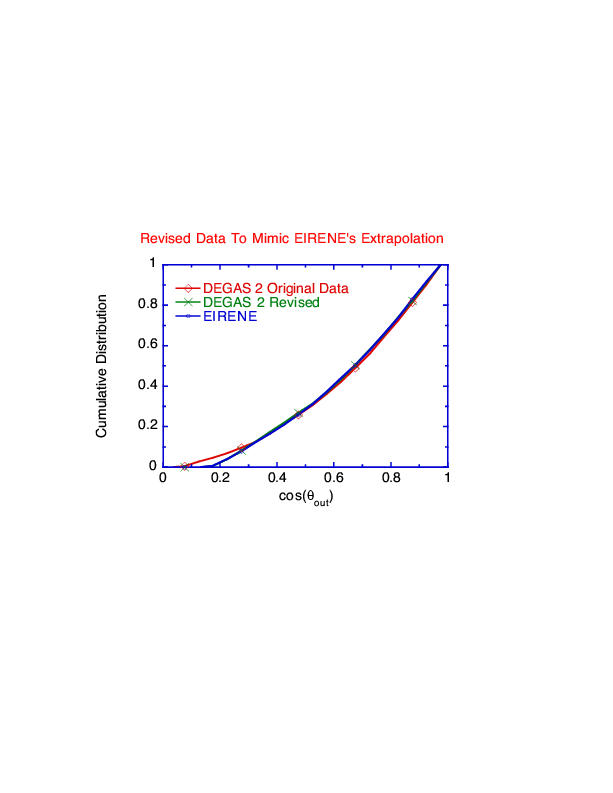
\includegraphics[width=5in]{costh}
\caption{Comparison of the cumulative distribution of reflected 
outgoing polar angles sampled in DEGAS 2 and EIRENE 
with the input data obtained from EIRENE's {\tt TRIM} file.
These distributions were compiled from all of the initial incident
{\em ions} (i.e., at the start of the flight) in a particular
zones. All of these ions strike the target normally with 6.88 eV.}
\label{costh}
\end{center}
\end{figure}

Figure~\ref{costh} shows the sampled cumulative distribution from two
DEGAS 2 runs and from an EIRENE run. These data were compiled from
all of the ions incident on the target in a particular zone (normal
incidence at 6.88 eV). The curve labeled ``original'' shows the DEGAS 2
treatment extending down to near $\cos(\theta_{\rm out}) \simeq 0$.
The ``revised'' curve demonstrates that our modifications to the DEGAS 2
data successfully mimic the EIRENE extrapolation behavior.


\subsection{H$_{2}$ Dissociation Rate}
\label{h2rate}

Significant differences in the electron energy sink were traced to
a discrepancy in the H$_{2}$ dissociation rate (reaction 2.2.5
in the Janev book\cite{Jane87}) at the lowest electron temperatures,
$T_{e} \simeq 1$ eV. Unfortunately, both the plot and the fit 
for these data in the Janev book are {\em wrong}. One needs
to refer to the corresponding preprint even to get the correct
values for the fit coefficients. EIRENE has those values, but applies
them down to the smallest $T_{e}$ used in the code, 1 eV. However,
the fit is valid down to only 1.2 eV. The dissociation rate values
used in DEGAS 2 at these lowest temperatures were taken directly from
the tabular data provided with the original DEGAS code\cite{Heif82},
not from the fit. The point is that these values differ from those
computed by the fit (presumably due to the fit not being valid there).
No record explaining the origin of the DEGAS values, but we assume
that they were taken from the initial data compilation from which the
fit was derived. Regardless, the remedy for the objectives of this
benchmark is to replace these low $T_{e}$ dissociation rates with the
same values used in EIRENE. The results of Sec.~\ref{outofthebox}
have the DEGAS values; runs discussed in subsequent sections will
have the EIRENE values.

\subsection{Estimator Differences}
\label{estdiffs}

With DEGAS 2 run as in Sec.~\ref{outofthebox}, the relative standard
deviations for the electron and ion energy sources were substantially
larger than those for EIRENE (these differences were most noticeable
close to the target). The cause of the higher electron energy
source variance was that DEGAS 2 was using a collision estimator
for the molecular contributions to that quantity (for historical reasons), 
while EIRENE was using a track length estimator. Switching the estimator
used in DEGAS 2 required a minor change to {\tt tallysetup} (see
Sec.~\ref{maincode}). At the same time, we changed the scoring of
the electron impact ionization of deuterium contributions to the ion
energy and momentum sources from being done ``post process''
(i.e., computed from the neutral density at the end of the run) to
a track length estimator. This allowed the variance contributions from
this process to be accounted for in these scores and was essential for
comparing with the EIRENE values (see Sec.~\ref{statcompare}).

The main reason for the larger ion energy source variance in DEGAS 2,
however, was that charge exchange was being treated by the collision
estimator, rather than the track length estimator used in EIRENE. 
The original reason for choosing the collision estimator in DEGAS 2
was that the charge exchange data file did not have the required
integrals of the cross section needed to score the energy and momentum
exchanges\cite{Reit93}. We have now worked out the forms these
integrals must have to emulate the EIRENE assumption of constant
$\sigma v$ and incorporated them into the charge exchange data file.
% Can add here variants of these expressions once we've documented
% the right expressions elsewhere.

The runs of Sec.~\ref{outofthebox} do not employ these estimator
changes (and utilize a different charge exchange cross section
altogether, as was noted previously), while runs in subsequent
sections have these modifications incorporated.

\subsection{Other Differences}
\label{otherdiffs}

We suspect that there are other differences remaining which will prevent
the two codes from being brought into closer agreement. For example,
DEGAS 2 uses a logarithmic interpolation in incident energy for the
Bateman format reflection data. EIRENE assumes a linear interpolation. 
The interpolation schemes in DEGAS 2 presently require a uniform
spacing, either linearly or logarithmically, between data points 
(a nonuniform spacing option was tried at one point, but abandoned
as too difficult to maintain). Hence, the interpolation technique
used by EIRENE cannot be emulated without significant changes to the
code. On the other hand, the subtlety of some of the differences which have
been detailed in this section suggests that remaining nonstatistical
discrepancies in the code results are unlikely to be of physical
significance and are consistent with minor numerical differences
between the codes.

\section{Characterize Comparison}

The principal means of comparing the code results is now considered to
be the quantitative prescription given in Sec.~\ref{statcompare}.
We will, however, begin this section with plots to illustrate two
points.

\subsection{Density Differences}

In Fig.~\ref{ddendiff}, we show the relative error,
\begin{equation}
\epsilon_{\rm rel} = \frac{n^{\rm D}_{D} - n^{\rm E}_{E}}{
\sigma_{\rm rsd}^{\rm D} \sqrt{(n^{\rm D}_{D})^{2} + (n^{\rm E}_{E})^{2}}}.
\end{equation}
This expression is equivalent to Eq.~(\ref{epsilonrel}) with $\sigma_{\rm rsd}$
being the relative standard deviation. Within the {\tt geomtesta} 
post-processor (see Sec.~\ref{maincode}), we do not have access to the
EIRENE error estimates (see Sec.~\ref{statcompare}). However, in the case
of the deuterium density, the EIRENE and DEGAS 2 relative standard
deviations are sufficiently similar that we can treat them as equal for
this purpose. Both are on the order of a one to a few percent near
the target. The scale in Fig.~\ref{ddendiff} indicates the number
of standard errors between the DEGAS 2 and EIRENE density values.
Note that this is a signed quantity. The white zones indicate areas
with differences greater than 3 times the standard error; the black 
areas indicate likewise that the lower bound has been exceeded.

\begin{figure}
% \epsfverbosetrue
\begin{center}
\leavevmode
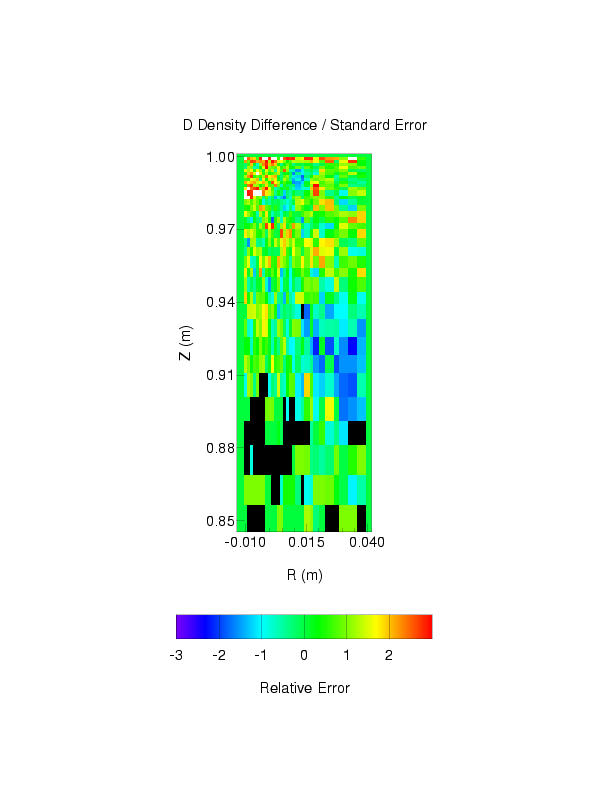
\includegraphics[width=5in]{ddendiff}
\caption{Difference between DEGAS 2 and EIRENE deuterium density relative
to the standard error estimate.}
\label{ddendiff}
\end{center}
\end{figure}

The dominance of the green areas is indicative of the nearly complete
statistical agreement (see Sec.~\ref{quantcompare}). The red, orange,
and yellow zones near the target likely point to a remaining systematic
discrepancy between the codes, as suggested in Sec.~\ref{otherdiffs}.

\subsection{Comparison of Momentum Source}

As indicated by Figs.~\ref{dmomsrc} and \ref{eirmomsrc}, the deuterium
ion parallel momentum sources computed by the two codes are qualitatively
(i.e., visually) similar. However, the statistical errors are extremely 
high (Fig.~\ref{momrsd}), presumably caused by the tight coupling with
the background ions through charge exchange (i.e., the net momentum
source due to charge exchange is the difference of two nearly equal
numbers).

\begin{figure}
% \epsfverbosetrue
\begin{center}
\leavevmode
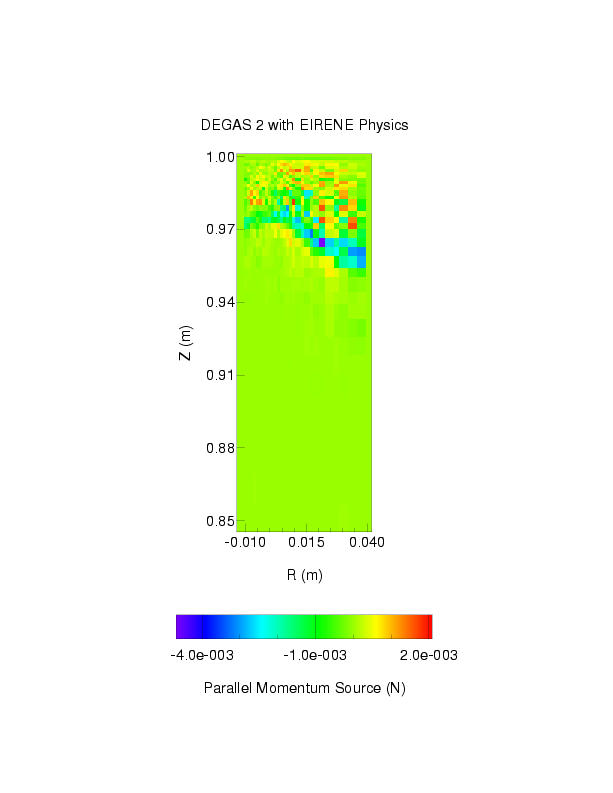
\includegraphics[width=5in]{d_mom_src}
\caption{Source of deuterium ion parallel momentum computed by DEGAS 2.}
\label{dmomsrc}
\end{center}
\end{figure}

\begin{figure}
% \epsfverbosetrue
\begin{center}
\leavevmode
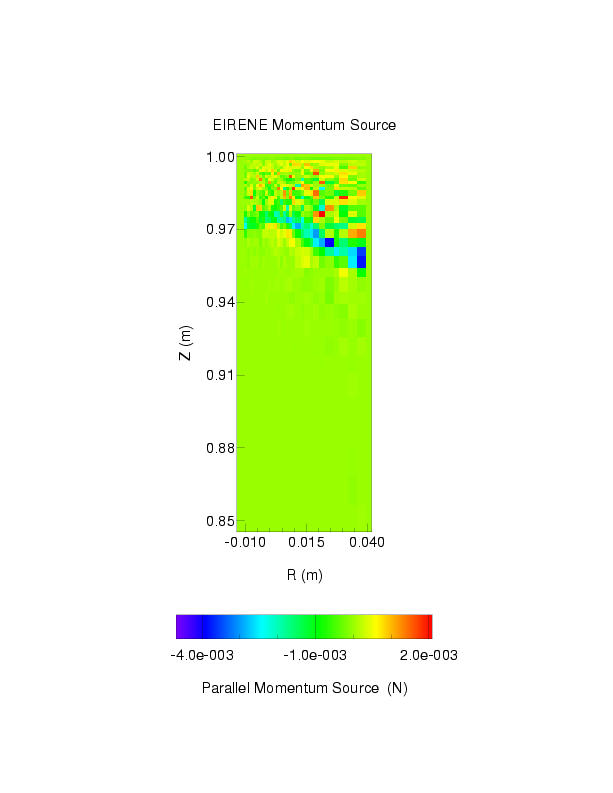
\includegraphics[width=5in]{eir_mom_src}
\caption{Source of deuterium ion parallel momentum computed by EIRENE.}
\label{eirmomsrc}
\end{center}
\end{figure}

\begin{figure}
% \epsfverbosetrue
\begin{center}
\leavevmode
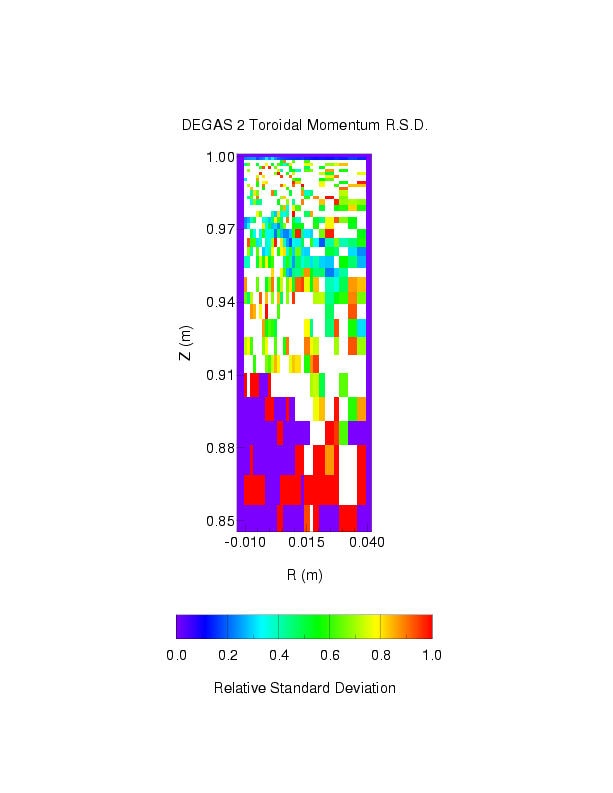
\includegraphics[width=5in]{mom_rsd}
\caption{Relative standard deviation for the deuterium ion momentum source
computed by DEGAS 2.}
\label{momrsd}
\end{center}
\end{figure}

The lack of regions with small relative standard deviations makes comparison
of the code results (see Sec.~\ref{statcompare}) problematic since we 
require a large number of (independent, ideally) zones with ``good
statistics'' (so that the Central Limit Theorem applies) for the analysis.
As will be seen in Sec.~\ref{quantcompare}, relaxing one of these two
constraints permits a comparison to be made. In each case, the results
are consistent with the two codes being in agreement. The deuterium ion 
energy source likewise has significant relative standard deviations, 
although smaller than those shown in Fig.~\ref{momrsd}. The consequences
for the stability of a coupling to a plasma transport code may be
more serious, however. Future work will assess and remedy this situation,
if necessary.

\subsection{Results of Quantitative Comparison}
\label{quantcompare}

The procedure outlined in Sec.~\ref{statcompare} must be amended slightly
to accomodate the remaining few-percent systematic differences in some
of the code results. The relative error is given instead by
\begin{equation}
\epsilon_{\rm rel} = \frac{\mu^{\rm D}_{K} - \mu^{\rm E}_{K^{\prime}}}
{\max{\left( \sqrt{(s^{\rm D}_{K})^{2} + (s^{\rm E}_{K^{\prime}})^{2}},
\sigma_{\rm min} \frac{\mu^{\rm D}_{K} + \mu^{\rm E}_{K^{\prime}}}{2}\right)}},
\end{equation}
where again the $s_{K}$ refers to the standard error for a simulation
of $K$ flights (i.e., $s_{K} = \sigma_{\rm rsd} \mu_{K}$). The 
additional parameter, $\sigma_{\rm min}$ is associated with the
statistical error (expressed as a fraction, like the relative
standard deviation). 

For all of these except the ion energy and momentum
source, $\sigma_{\rm max} = 20 \%$ and $\sigma_{\rm min}$ is given.
For those two, $\sigma_{\rm min} = 0$ and $\sigma_{\rm max}$ is given.
In the former case, the relative standard deviation is required to be
$< 20 \%$ to ensure that the Central Limit Theorem is applicable and
$\sigma_{\rm min}$ represents the systematic error. Of the tested
values of $\sigma_{\rm min}$ the one which yields a set of percentages
most closely matching the Maxwellian ideal ($68 \%$, $95 \%$, $99.7 \%$)
is taken as our estimate of the systematic error. For the ion energy
and momentum sources, we are unable to get ``good statistics'' with
$\sigma_{\rm max} = 20 \%$; hence, larger values are tested. The
relative standard deviations are too large for any systematic error
to be detected, so we use $\sigma_{\rm min} = 0$.

\begin{tabular}{|c||c|c|c||c|c|c|}
\hline
 Source:       & \multicolumn{3}{|c||}{Plate} & \multicolumn{3}{|c|}{Recombination} \\ \hline  % Do better?
        & $1 \sigma$ & $2 \sigma$ & $3 \sigma$ & $1 \sigma$ & $2 \sigma$ & $3 \sigma$ \\ \hline
\multicolumn{7}{|l|}{D Density} \\ \hline
$\sigma_{\rm min}=7 \%$ & $82 \%$ & $99.2 \%$ & $100  \%$ & $90 \%$ & $99.4 \%$ & $99.9 \%$ \\ \hline
$\sigma_{\rm min}=5 \%$ & $75 \%$ & $95   \%$ & $99.8 \%$ & $82 \%$ & $98   \%$ & $99.9 \%$ \\ \hline
$\sigma_{\rm min}=0 \%$ & $56 \%$ & $86   \%$ & $96   \%$ & $52 \%$ & $88   \%$ & $99   \%$ \\ \hline
\multicolumn{7}{|l|}{D$_{2}$ Density} \\ \hline
$\sigma_{\rm min}=0 \%$ & $64 \%$ & $92 \%$ & $98   \%$ & $59 \%$ & $92 \%$ & $99.2 \%$ \\ \hline
\multicolumn{7}{|l|}{D$_{2}^{+}$ Density} \\ \hline
$\sigma_{\rm min}=0 \%$ & $63 \%$ & $92 \%$ & $100  \%$ & $68 \%$ & $97  \%$ & $100  \%$ \\ \hline
\multicolumn{7}{|l|}{D$^{+}$ Ion Source Rate} \\ \hline
$\sigma_{\rm min}=7 \%$ & $74 \%$ & $99.6 \%$ & $100  \%$ & $83 \%$ & $99.3 \%$ & $100  \%$ \\ \hline
$\sigma_{\rm min}=5 \%$ & $57 \%$ & $94   \%$ & $100  \%$ & $63 \%$ & $98   \%$ & $99.8 \%$ \\ \hline
$\sigma_{\rm min}=0 \%$ & $38 \%$ & $73   \%$ & $93   \%$ & $38 \%$ & $66   \%$ & $85   \%$ \\ \hline
\multicolumn{7}{|l|}{Electron Energy Source Rate} \\ \hline
$\sigma_{\rm min}=7 \%$ & $92 \%$ & $99 \%$ & $99.1 \%$ & $93 \%$ & $99 \%$ & $99.3 \%$ \\ \hline
$\sigma_{\rm min}=5 \%$ & $79 \%$ & $98 \%$ & $99.1 \%$ & $86 \%$ & $98 \%$ & $99.1 \%$ \\ \hline
$\sigma_{\rm min}=0 \%$ & $38 \%$ & $72 \%$ & $91   \%$ & $45 \%$ & $78 \%$ & $94   \%$ \\ \hline
\multicolumn{7}{|l|}{D$^{+}$ Ion Energy Source Rate} \\ \hline
$\sigma_{\rm max}=70 \%$ & $69 \%$ & $94 \%$ & $99   \%$ & $68 \%$ & $96 \%$ & $99.7 \%$ \\ \hline
$\sigma_{\rm max}=50 \%$ & $69 \%$ & $94 \%$ & $99.1 \%$ & $65 \%$ & $97 \%$ & $100  \%$ \\ \hline
$\sigma_{\rm max}=20 \%$ & $68 \%$ & $94 \%$ & $100  \%$ & $61 \%$ & $98 \%$ & $100  \%$ \\ \hline
\multicolumn{7}{|l|}{D$^{+}$ Ion Parallel Momentum Source Rate} \\ \hline
$\sigma_{\rm max}=70 \%$ & $72 \%$ & $88 \%$ & $99.2 \%$ & $75 \%$ & $92  \%$ & $99.4 \%$ \\ \hline
$\sigma_{\rm max}=50 \%$ & $74 \%$ & $97 \%$ & $100 \%$ & $76 \%$ & $97  \%$ & $99   \%$ \\ \hline
$\sigma_{\rm max}=20 \%$ & $58 \%$ & $89 \%$ & $100 \%$ & $0  \%$ & $0   \%$ & $0    \%$ \\ \hline
\end{tabular}

The two molecular densities fare the best, given nearly Maxwellian percentages
without allowing for any systematic error. The atom density,  electron
energy source (which is given by the atom density times a function of $T_{e}$,
apart from a small contribution due to molecules), and ion
source rate are all roughly consistent
with a $5 \%$ systematic error. Again, the ion energy and momentum sources
are too noisy to permit an estimate of the systematic error. However, these
numbers indicate that the two codes do agree within the estimated
statistical errors.

\section{Performance Benchmark and Optimization}
\label{performance}

Although efficiency was kept in mind during all
stages of the design process, no effort was made to optimize the
performance of DEGAS 2 along the way.
In this section, we describe the benchmark of the code's performance against 
EIRENE. Speed bottlenecks were discovered through profiling. 
Improvements eliminating those bottlenecks.were implemented.
Some involved
significant code revisions; others were
effected by simple changes to source or
input files. The end result was that the run time for DEGAS 2 was 
roughly equal to
that of EIRENE within the variations normally experienced in a time-sharing
environment.

The implemented code revisions were motivated by profiling the code to
determine which subroutines were the most time-consuming. At one point,
assignments and comparisons of string variables were using significant
fractions of the run time. The strings responsible were 
being used to 
describe auxiliary data associated with the atomic physics reactions.
The code was modified to compile a list of all of these strings at the
beginning of the run and to use an integer pointer into that list for
the run-time comparisons and assignments. Because these code changes
were pervasive, their impact on the run time could not be documented
as carefully as the other improvements noted below. Roughly, however,
they resulted in a reduction of about 10 seconds per 
1000 flights.

\subsection{Starting Point}

The starting assumptions were the same as those associated with the
code as run for the initial EIRENE benchmark (specifically, the 
DEGAS 2 version with the CVS tag \verb+V1_8a+).
The ``EIRENE physics'' set was used to minimize differences due to the 
number of collisions and to permit direct comparisons of the variances.

For each code configuration, runs were performed at 1000, 2000, and
4000 flights. The time for the 1000 flight case was subtracted from
the other two and the results used to estimate the incremental
time required to track 1000 flights. The idea is that production
runs would be substantially longer than these (with relative standard
deviations on the order of $1 \%$) so that the overhead associated with
input and output would be negligible. In a few cases, production length
runs (e.g., 80,000 flights) were done; for those, the run time was just
taken to be the time consumed divided by 80. 

These runs were performed on a Sun UltraSPARC 2 running SunOS 5.5.1
and V. 4.2 of f77 with \verb+-O4+ optimization. Again, because this computer 
is a time-sharing system, these run times are only approximate. The 
estimated error is about $10 \%$. The baseline run time for
DEGAS 2 was: 136 seconds per 1000 flights.

\subsection{Charge Exchange Rejection}

The charge exchange cross section depends on the relative ion-neutral
velocity. However, collisions are decided upon using a cross section
averaged over a Maxwellian distribution. In the baseline, the ion
collision partners were chosen so as to be consistent with the actual
cross section using a rejection technique, sampling several ions 
before finding one which is satisfactory.
The version of EIRENE used in this benchmark does not do this 
(neither did the original DEGAS). 

For the
first change, charge exchange rejection was turned off. A cursory
examination of the results showed no significant impact on the neutral
density. However, a stronger effect may have occurred elsewhere (e.g.,
energy transferred to background species). Run time after disabling
charge exchange rejection: 119 seconds per 1000 flights.

\subsection{Reduce Number of Scores}

One impressive feature of EIRENE is how thoroughly its default operation
has been pared down to the minimum necessary for coupling to the fluid
plasma codes. In particular, no data on the variances are kept. DEGAS 2 was
written with the philosophy that the mean value for a score is meaningless
without a corresponding variance, and the two data values are kept
together. For this comparison, a short list of variances was requested
in the EIRENE input file. These will be needed later.

As presently distributed, DEGAS 2 by default sets up about 14 scores or
tallies. This list was reduced to 7 at this step (later, 3 more will
be eliminated leaving the neutral density and the 3 scores representing
the particle, momentum, and energy transfer to the background species).
Run time after cutting the number of scores to 7: 95 seconds per
1000 flights.

\subsection{Compression of Scores}

The first offender in the profiling exercise was the routine responsible
for compiling the scores accumulated during a single flight into the
global total. As originally written, both the total and incremental
scoring arrays were full-sized (roughly the
number of zones times the number of scores times the number of
background species). However, each flight visits only a small fraction
of the problem space, and this routine was spending a significant
amount of time adding $0$ to $0$.

These scoring arrays were modified to contain only the non-zero scores,
with an array of pointers mapping their contents back to the corresponding
locations in the full-sized arrays (which were still used for the
final output stage). Run time after implementation of compressed
scoring: 49 seconds per 1000 flights.

\subsection{Other Changes with Minimal Effects}

Further reducing the number of scores from  7 to 4 
had little impact on
the run, probably because of the use of
compression at this point.

DEGAS 2 (and EIRENE) employ a 10 term quadratic representation of all
surfaces in the geometry. 
In some problems, such as this one, only the linear terms
are needed. The inclusion of the quadratic terms was made a compile-time
option so that they could be turned off for fully linear geometries.
Earlier tests of the impact of this change showed a reduction of
about 4 seconds per 1000 flights. However, in this more systematic
series of trials, the improvement could not be quantified with certainty.

\subsection{Variance-Altering Changes}

Thus far, all of the changes made led to the same final results as
the run with ``EIRENE physics''.
Most of the subsequent changes,
while reducing the run time, also result in increases
in the variance of the results. In a given Monte Carlo calculation,
the variance is inversely proportional to the number of flights and, hence,
to the run time. So, the performance Figure of Merit (FOM) is the
variance times the run time.  An attempt will be made
below to quantify this FOM, but we can also compare qualitatively the
variance over the most relevant portion of the problem space (near the
target plate) via the relative standard deviation $\sigma_{\rm rsd}$. 
Figure~\ref{densityrsd} shows $\sigma_{\rm rsd}$ for the deuterium density
in the baseline case.

\begin{figure}
\begin{center}
\leavevmode
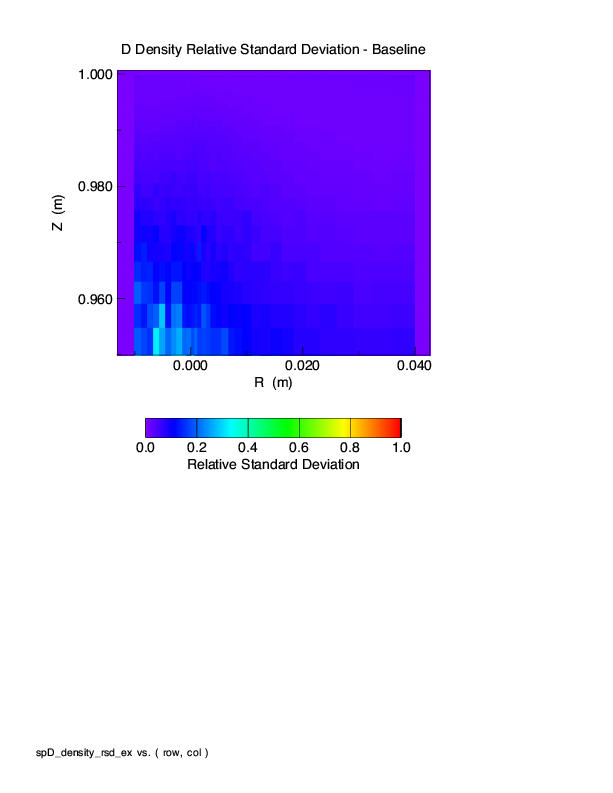
\includegraphics[width=5in]{spD_density_rsd_ex}
\caption{Relative standard deviation of the atomic deuterium density in the
baseline run of the performance benchmark.}
\label{densityrsd}
\end{center}
\end{figure}

Below we will use $\sigma_{\rm rsd}$ for the source rate of D$^{+}$ 
due to ionization
of neutrals. Although not computed for this baseline run, this
$\sigma_{\rm rsd}$ should
be comparable to that shown in Fig.~\ref{densityrsd} except for the 
first one or two zones adjacent to the plate
in which the contributions from D$_{2}$ are significant.

\subsection{Removal of Suppressed Ionization}

The simplest (``analog'') Monte Carlo simulation kills off neutrals
at their first ionizing collision. However, this makes finding the
solution more than one mean free path from the source difficult. The
predominant non-analog improvement is to assign a weight to each neutral
flight (e.g., initially 1) and reduce that weight at each step to reflect
the amount of ionization which should have occurred along the way. 
As a result, smaller variances are obtained in low probability regions of
the problem. Because each flight will thus be tracked for more steps, 
a run using suppressed ionization will take longer. Whether or not
that time is well spent depends on the problem at hand.

These EIRENE runs do not use suppressed ionization. For the purposes
of comparison, we turned it off in DEGAS 2 as well. The run time
without suppressed ionization dropped to 15 seconds per 1000 flights.
Figure~\ref{ionsourceisrsd} shows the resulting $\sigma_{\rm rsd}$.

\begin{figure}
\begin{center}
\leavevmode
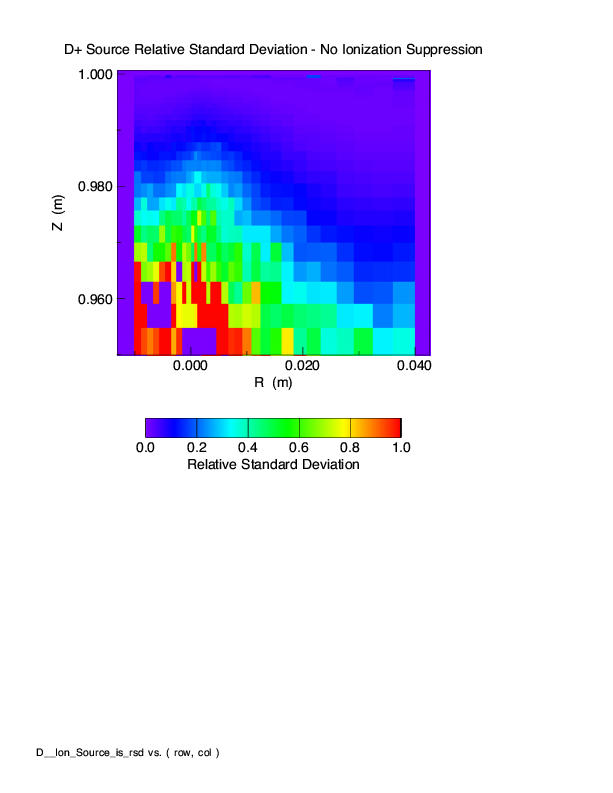
\includegraphics[width=5in]{D__Ion_Source_is_rsd}
\caption{Relative standard deviation of the D$^{+}$ ion source {\em without}
suppressed ionization.}
\label{ionsourceisrsd}
\end{center}
\end{figure}

\subsection{Collision Estimator}

Some of the scores in DEGAS 2, e.g., the neutral density and the D$^{+}$ source
rate, are computed via the track-length estimator. The other scores
are compiled using data only at collisions (though most of these can also
be done by track-length). Since the collision routines get executed
regardless of whether or not the resulting data are used in the scores, we
felt that it would be interesting to switch all of the estimators to 
collision (except density) and eliminate the overhead associated with
generating the track-length scores. Of course, doing this increases the
variance as is shown in Fig.~\ref{ionsourcecolrsd}. The run with using
the collision estimator (again without suppressed absorption) needed
10 seconds per 1000 flights.

% NOTE: it's not clear from my original text which options were used
% in this section and the next - are all of these time reductions essentially
% additive?

\begin{figure}
\begin{center}
\leavevmode
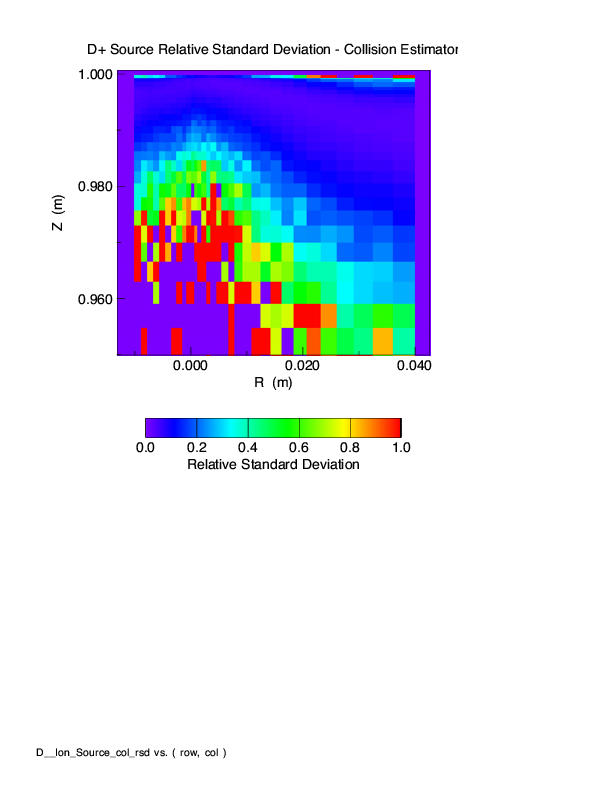
\includegraphics[width=5in]{D__Ion_Source_col_rsd}
\caption{Relative standard deviation of the D$^{+}$ ion source using 
a collision estimator and {\em without}
suppressed ionization.}
\label{ionsourcecolrsd}
\end{center}
\end{figure}

\subsection{Russian Roulette for Molecules}

Two of the seven reactions involving D$_{2}$ and D$_{2}^{+}$ in 
DEGAS 2 result in two D
atoms. DEGAS 2 normally tracks both of these. EIRENE, however, like the
original DEGAS, chooses one of the two to follow and ``kills'' off the other.
This is a simple example of a general nonanalog Monte Carlo technique known
as ``Russian roulette''. Whether the use (or non-use) of this technique 
improves the variance again depends on the problem. For the purposes of
this benchmark, Russian roulette was added to DEGAS 2's molecular 
dissociation routine. Those scores switched to collision estimator in the
previous section were reverted to the track-length estimator for this
configuration. Figure~\ref{ionsourcerrrsd} shows the corresponding
$\sigma_{\rm rsd}$. This run used only 8 seconds per 1000 flights.

\begin{figure}
\begin{center}
\leavevmode
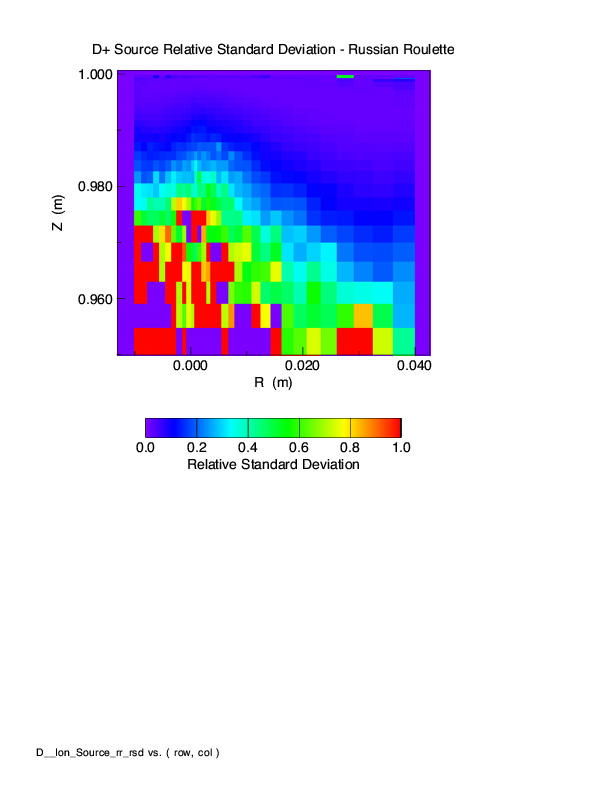
\includegraphics[width=5in]{D__Ion_Source_rr_rsd}
\caption{Relative standard deviation of the D$^{+}$ ion source using 
Russian roulette for molecules.}
\label{ionsourcerrrsd}
\end{center}
\end{figure}

\subsection{Figures of Merit}

We now have four different configurations with which to evaluate this
figure of merit, variance times run time. Presently, there is no single
``answer'' in these simulations which we can use to compute the FOM. 
Somewhat arbitrarily, we have selected a region of the problem spanning
the width (radius) of this geometry and encompassing most of the integrated
D$^{+}$ source (the selection was made by eyeballing the plot; $83 \%$ of the
integrated source was included). The $\sigma_{\rm rsd}$ for each
configuration was divided by that of the baseline and integrated over this
region. We then defined the FOM as the product of the 1000
flight run times (quoted above) and the square (to get the variance) of
this ratio.

\begin{tabular}{|c|c|c|c|}
\hline
Configuration & Seconds / 1000 flights & $\sigma_{\rm rsd}$ ratio & FOM \\ \hline 
Baseline      &             49         &     1.0               &  49 \\ \hline
No Suppressed Ionization &  15         &     1.9               &  54 \\ \hline
Collision Estimator      &  10         &     4.3               & 185 \\ \hline
D$_{2}$ Russian Roulette &   8         &     2.3               &  41 \\ \hline
\end{tabular}

Clearly, using the collision estimator is not a good idea. The effectiveness
of suppressed ionization could go either way. However, doing Russian
roulette on the molecular products (this run was done without ionization
suppression) looks to be the overall winner. Probably not by accident, this
configuration is the closest to the default mode of operation for EIRENE.

\subsection{EIRENE Performance}

Of course, the whole point of this portion of the benchmark is to compare
the performance of DEGAS 2 against that of EIRENE. Apart from the addition
of the variance output to EIRENE, no other modifications have been made to
its default mode of operation. However, the compiler optimization was
changed from the \verb+-O3+ value specified with the IPP-Garching version
to the \verb+-O4+ which appears to work well for DEGAS 2 with the Sun
FORTRAN 77 compiler. Over several runs of length 1000 to 10000 flights,
the incremental time for 1000 flights is 12 seconds. 
The relative standard deviations computed by EIRENE were consistent with
those of the corresponding DEGAS 2 configuration (Russian roulette), 
although a direct comparison was not made here (see
Sec.~\ref{estdiffs}). 

Within normal variations, the two codes are thus running at the same
speed. The particular DEGAS 2 configuration should be chosen according to
the needs of the problem at hand. Keep in mind that the original objective of
DEGAS 2 was to be faster than DEGAS; the hope was that the code would
yield performance comparable to that of EIRENE while retaining
flexibility. That objective has been met. DEGAS 2 is also able
to take full advantage of the substantial 
benefits of parallel processing.

Note, however, that EIRENE's computation of variances is less 
than optimal. Disabling them in the input file and turning off
unneeded tallies reduces the incremental run time to 3 seconds
per 1000 flights. At this point, EIRENE is substantially faster than 
DEGAS 2 since turning off
its variance computation (which has been optimized) will not have a significant
impact. The performance comparison between the two codes will
be revisited as part of a later benchmark utilizing a
more realistic divertor geometry.

The advantages of dynamic memory allocation of all
run-time arrays, another design feature of DEGAS 2, have also been
demonstrated during this benchmark. The run-time sizes were: DEGAS 2 -
7 MB, EIRENE - 142 MB. By reducing the dimensioning parameters in EIRENE to 
values more
appropriate for this input file, the size of the code was reduced from
142 MB to 55 MB.

\chapter{Future Work}

\section{To Do List}

The following are known problems and / or are items which need
to be done:

\begin{itemize}
\item Sampling from a drifting Maxwellian is fudged or not done at all
(sampling recycling ion, recombining ion, charge exchange).
\item H / H2 fraction for gas puffing is not implemented; needed for
wall desorption, too.
\item Need real sheath physics routine.
\item Add fits to reactions, as done for PMI.
\item Use FWEB to break up reaction-specific routines into separate files.
\item Generalize detectors to treat finite solid angle?
\item Might be able to replace eval\_data and pd\_eval\_data with a single
routine.
\item Generalize setup of detector views to permit chords not lying in poloidal
plane.
\item Need to add other H\_alpha emitting molecular reactions (will follow
EIRENE here, unlike DEGAS, and explicitly track these reactions rather
than fudging the emission rates of the dominant reactions).
\item In readgeometry, set up detector views using chords from DEGAS input 
file.
\item Note: in readgeometry, improved treatment of double-null, vacuum, UEDGE
option, but didn't do likewise for !vacuum case: it will probably not
work.
\item Manual and other documentation needs to be updated.
\item Add a dump of trajectories? Charles says that we might even be able to
plot these in real time using some MPI-based utilities.
\item Define default PMI packages which are invoked based on all material and
test pairs. Ideally, the user should be presented with the list compiled
at problemsetup time and edit it prior to actually running problemsetup.
\item Extend sector definition to use two surfaces and a zone. If needed,
this could be an ordered pair with the second member optional (or duplicated).
Do this only if it cleans up some of the ugly sector related code in
readgeometry and sector scoring routines.
\item Adapt DG to write DEGAS 2 geometry netCDF file.
\item Begin development of hybrid kinetic-fluid neutral transport code.
\end{itemize}

\chapter{Troubleshooting}

\section{Help!}
\label{help}

If you're really in need of help, try contacting \\
Charles Karney \\
Princeton Plasma Physics Laboratory, MS 28 \\
P. O. Box 451 \\
Princeton NJ 08543-0451 \\ 
(609) 243-2607 \\
\href{mailto:karney@pppl.gov}{E-mail: karney@pppl.gov}

or

Daren Stotler \\
Princeton Plasma Physics Laboratory, MS 27 \\
P. O. Box 451 \\
Princeton NJ 08543-0451 \\ 
(609) 243-2063 \\
\href{mailto:dstotler@pppl.gov}{E-mail: dstotler@pppl.gov}

\begin{thebibliography}{99}
\bibitem{Tend87}The development of analytic, numerical, and Monte Carlo  
methods of solving
the time-independent Boltzmann equation describing neutral kinetics is
reviewed in: \\ M. Tendler and D. Heifetz, {\em Fusion Tech.} {\bf 11}, 289 
(1987).
\bibitem{Span69} The ``bible'' of Monte Carlo transport techniques is: \\
J. Spanier and E. M. Gelbard, ``MonteCarlo Principles and Neutron
Transport Problems'' (Addison-Wesley Publishing Company, Reading
Massachusetts, 1969). \\
Other references from the neutron transport field include: \\
J. M. Hammersley and D. C. Handscomb, ``Monte Carlo Methods'' (Metuchen,
London, 1964). \\
L. L. Carter and E. D. Cashwell, ``Particle-Transport Simulation with the
Monte Carlo Method'' (National Technical Information Service, Springfield,
Virginia, 1975). \\
Ivan Lux and Laszlo Koblinger, ``Monte Carlo Particle Transport Methods:
Neutron and Photon Calculations'' (CRC Press, Boca Raton, 1991).
\bibitem{Heif82} The Algorithm and applications of DEGAS are discussed in: \\
D. Heifetz, D. Post, M. Petravic, J. Weisheit, and G. Bateman,
{\em J. Comp. Phys.} {\bf 46} 309 (1982). \\
The Proceedings from a NATO-sponsored school in Val-Morin, Canada (1984)
are an invaluable reference for scrape-off layer physics. In addition
to again describing the algorithms and applications of DEGAS, Heifetz
covers in his article some of the basics of neutral transport in a plasma:
D. B. Heifetz, in {\em Physics of Plasma-Wall Interactions in Controlled 
Fusion}, D. Post and R. Behrisch, Eds., (Plenum, New York, 1986), p. 695.
\bibitem{Stot92} D. P. Stotler et al., {\em J. Nucl. Mater.}
{\bf 196-198}, 894 (1992).
\bibitem{Bate61} D. R. Bates, A. E. Kingston, and R. W. P. McWhirter,
{\em Proc. R. Soc. A} {\bf 267}, 297 (1962).
\bibitem{McWh65} R. W. P. McWhirter, in {\em Plasma Diagnostic Techniques},
R. H. Huddlestone and S. L. Leonard, Eds. (Academic, New York, 1965).
\bibitem{FWEB} \verb+http://w3.pppl.gov/~krommes/fweb_toc.html+
(\href{http://w3.pppl.gov/~krommes/fweb_toc.html}{FWEB home page})
\bibitem{nCDF} \verb+http://www.unidata.ucar.edu/packages/netcdf/index.html+
(\href{http://www.unidata.ucar.edu/packages/netcdf/index.html}{netCDF home page})
\bibitem{HDF} \verb+http://hdf.ncsa.uiuc.edu/+
(\href{http://hdf.ncsa.uiuc.edu/}{HDF home page})
\bibitem{Reit92} Although never formally published and not readily 
available online, the EIRENE User's Manual is a very useful reference on 
the physics and algorithms of Monte Carlo neutral transport: \\
D. Reiter, ``The EIRENE Code, Version: Jan. 92, Users Manual'', EURATOM-KFA
Institut f\"{u}r Plasmaphysik Report JUL-2599 (1992). \\
One source for a recent version of this document is the ``SOLPS'' package
maintained R. Schneider and D. Coster of the Max Planck Insitut f\"{u}r 
Plasmaphysik in Garching. Try the 
\verb+http://www.rzg.mpg.de/~dpc/solps.html+  
\href{http://www.rzg.mpg.de/~dpc/solps.html}{SOLPS home page} for more
information.
\bibitem{Case67} K. M. Case
and P. F. Zweifel, {\em Linear Transport Theory} (Addison-Wesley, Reading, MA,
1967).
\bibitem{Stot96} D. P. Stotler, A. Yu. Pigarov, C. F. F. Karney, 
S. I. Krasheninnikov, B. LaBombard, B. Lipschultz, G. M. McCracken,
A. Niemczewski, J. A. Snipes, J. L. Terry, and R. A. Vesey, in {\em 
Fusion Energy 1996} (Proc. 16th Int. Conf. Montreal, 1996), Vol. 2 
(IAEA, Vienna, 1997) p. 633 (see also the corresponding
\href{http://www-local.pppl.gov/pppl/services/pub_report/1997/PPPL-3221-abs.html}{PPPL Report}).
  \bibitem{Jane87} R. K. Janev, W. D. Langer, K. Evans, Jr., and D. E. Post, Jr., {\em Elementary
Processes in Hydrogen-Helium Plasmas} (Springer-Verlag, Berlin, 1987)
(see also the corresponding \href{http://www-cfadc.phy.ornl.gov/aladdin/aladdin_list.html}{Aladdin data file}).
\bibitem{Reit93} D. Reiter, in {\em Atomic and Plasma-Material Interaction
Processes in Controlled Thermonuclear Fusion}, R. K. Janev and H. W.
Drawin, Eds., (Elsevier, New York, 1993), p. 243.
\bibitem{Jane93} R. K. Janev and J. J. Smith, {\em Atomic and Plasma-Material
Interaction Data for Fusion} (Supplement to the journal Nuclear
Fusion) {\bf 4} (1993) (see also the corresponding \href{http://www-cfadc.phy.ornl.gov/aladdin/aladdin_list.html}{Aladdin data file}).
\bibitem{John73} L. C. Johnson and E. Hinnov, {\em J. Quant. Spectrosc.
Radiat. Transfer} {\bf 13}, 333 (1973).
\bibitem{Weis75} J. C. Weisheit, {\em J. Phys. B: Atom. Molec. Phys.} {\bf 8},
2556 (1975).
\bibitem{Kanz00} R. J. Kanzleiter, D. P. Stotler, C. F. F. Karney, and 
D. Steiner {\em Phys. Plasmas} {\bf 7}, 5064 (2000).
\bibitem{Krst98} P. S. Krstic and D. R. Schultz, {\em Atomic and 
Plasma-Material Data for Fusion} {\bf 8}, 1 (1998).
\bibitem{Bach95} P. Bachmann and d. Reiter, {\em Contrib. Plasma Phys.} 
{\bf 35}, 45 (1995).
\bibitem{Abou91} H. H. Abou-Gabal and G. A. Emmert, {\em Nucl. Fusion}
{\bf 31}, 407 (1991).
\bibitem{Dalg58} A. Dalgarno, {\em Phil. Trans. R. Soc. London, Ser. A}
{\bf 250}, 426 (1958).
\bibitem{Hols52} T. Holstein, {\em J. Phys. Chem.} {\bf 56}, 832 (1952).
\bibitem{Wade79} J. M. Wadehra, {\em Phys. Rev. A} {\bf 20}, 1859 (1979).
\bibitem{Mayxx} Chr. May, Ph. D. Thesis. 
\bibitem{Reit97} D. Reiter, Chr. May,
M. Baelmans, and P. B\"{o}rner, {\em J. Nucl. Mater.} {\bf 241}, 342 (1997).
\bibitem{Chap70} S. Chapman and T. G. Cowling, {\em The Mathematical
Theory of Non-Uniform Gases} (Cambridge University Press, 1970).
\bibitem{Mors63} T. F. Morse, {\em Phys. Fluids} {\bf 6}, 1420 (1963).
\bibitem{Reid87} R. C. Reid, J. M. Prausnitz, B. E. Poling, {\em The
Properties of Liquids and Gases} (McGraw-Hill Book Company, New York, 1987).
\bibitem{CRC} {\em CRC Handbook of Chemistry and Physics, 75th Edition,
1913--1995}, D. R. Lide, Ed., p. 6-239 (CRC Press, Boca Raton, 1994).
\bibitem{Bevi69} P. R. Bevington, {\em Data Reduction and Error Analysis
for the Physical Sciences} (McGraw-Hill Book Company, New York, 1969).
\bibitem{Ecks91} W. Eckstein, {\em Computer Simulation of Ion-Solid
Interactions} (Springer-Verlag, New York, 1991).
\bibitem{Bate80} G. Bateman, ``Distribution of Neutrals Scattered Off 
A Wall'', PPPL Applied Physics Division Report \# 1 (1980).
\bibitem{Macm67} D. B. Macmillan, {\em SIAM J. Appl. Math.} {\bf 15}, 264 
(1967).
\bibitem{Span66} J. Spanier, {\em SIAM J. Appl. Math.} {\bf 14}, 702 (1966).
\bibitem{Knuth97} D. E. Knuth, {\em The Art of Computer Programming} 
(Addison-Wesley, Reading, MA, 1997).
\end{thebibliography}


%%tth:\printindex

\begin{theindex}

  \item adsorption, \hyperpage{41}
  \item Allocation, memory, \hyperpage{2}
  \item Atomic physics, \hyperpage{18}

  \indexspace

  \item background species, \hyperpage{41}
  \item BGK, \hyperpage{27}
  \item Boltzmann equation, \hyperpage{1}
  \item boxgen, \hyperpage{37}

  \indexspace

  \item Charge exchange, \hyperpage{22}
  \item chargex, \hyperpage{40}
  \item collisional-radiative, \hyperpage{18}
  \item CVS, \hyperpage{3}, \hyperpage{43}

  \indexspace

  \item dataexam, \hyperpage{38}
  \item datasetup, \hyperpage{37}
  \item DEGAS, \hyperpage{2}
  \item desorption, \hyperpage{41}
  \item Differential cross section, \hyperpage{22}
  \item Diffusion, \hyperpage{27}
  \item Diffusion cross section, \hyperpage{22}
  \item dissoc, \hyperpage{40}
  \item dissoc\_rec, \hyperpage{40}
  \item Distribution, probability, \hyperpage{5}

  \indexspace

  \item elastic, \hyperpage{40}
  \item Elastic scattering, \hyperpage{22}
  \item elements\_infile, \hyperpage{40}
  \item elementsfile, \hyperpage{40}

  \indexspace

  \item flighttest, \hyperpage{35}
  \item FWEB, \hyperpage{2}, \hyperpage{44}

  \indexspace

  \item Generators, random number, \hyperpage{5}
  \item generic, \hyperpage{40}
  \item generic PMI, \hyperpage{41}
  \item generic reactions, \hyperpage{40}
  \item geometry.inp, \hyperpage{42}
  \item geomtesta, \hyperpage{35}

  \indexspace

  \item HDF, \hyperpage{3}

  \indexspace

  \item ionization, \hyperpage{18}
  \item ionize, \hyperpage{40}
  \item ionize\_suppress, \hyperpage{40}

  \indexspace

  \item Macros, \hyperpage{2}
  \item matcheir, \hyperpage{39}
  \item matchout, \hyperpage{39}
  \item materials\_infile, \hyperpage{41}
  \item materialsfile, \hyperpage{41}
  \item Maxwell molecules, \hyperpage{27}
  \item Monte Carlo, \hyperpage{5}

  \indexspace

  \item NetCDF, \hyperpage{3}
  \item netCDF, \hyperpage{44}
  \item Neutral Transport, \hyperpage{1}
  \item Neutral-ion scattering, \hyperpage{22}
  \item Neutral-neutral scattering, \hyperpage{27}
  \item non-generic PMI, \hyperpage{41}
  \item non-generic reactions, \hyperpage{40}

  \indexspace

  \item Object oriented programming, \hyperpage{2}
  \item outputscript, \hyperpage{42}

  \indexspace

  \item Pcl-cvs, \hyperpage{43}
  \item PMI, \hyperpage{41}
  \item pmi\_infile, \hyperpage{41}
  \item pmitest, \hyperpage{38}
  \item pmiwrite, \hyperpage{37}
  \item problem\_infile, \hyperpage{41}
  \item problemfile, \hyperpage{41}
  \item problemsetup, \hyperpage{35}
  \item Processing, parallel, \hyperpage{3}

  \indexspace

  \item Random, \hyperpage{5}
  \item randomtest, \hyperpage{38}
  \item ratecalc, \hyperpage{37}
  \item rates, atomic physics, \hyperpage{18}
  \item reaction type, \hyperpage{40}
  \item reaction\_infile, \hyperpage{40}
  \item reactionfile, \hyperpage{40}
  \item reactiontest, \hyperpage{38}
  \item reactionwrite, \hyperpage{37}
  \item readbackground, \hyperpage{35}
  \item readbackground input, \hyperpage{42}
  \item readgeometry, \hyperpage{35}
  \item readgeometry input, \hyperpage{42}
  \item recombination, \hyperpage{18}, \hyperpage{40}
  \item reference level, \hyperpage{41}
  \item reflection, \hyperpage{41}

  \indexspace

  \item Scattering angle, \hyperpage{22}
  \item Scoring, \hyperpage{5}
  \item sourcetest, \hyperpage{38}
  \item species, \hyperpage{40}
  \item species\_infile, \hyperpage{40}
  \item speciesfile, \hyperpage{40}
  \item Spin exchange, \hyperpage{22}
  \item subset data, \hyperpage{41}
  \item symbolic name, \hyperpage{39}
  \item sysdeptest, \hyperpage{38}

  \indexspace

  \item Tags, \hyperpage{45}
  \item tally, \hyperpage{42}
  \item tally\_infile, \hyperpage{42}
  \item tallyfile, \hyperpage{42}
  \item tallysetup, \hyperpage{35}, \hyperpage{42}
  \item test species, \hyperpage{41}
  \item Theory, transport, \hyperpage{1}
  \item Total cross section, \hyperpage{22}
  \item Tracking, \hyperpage{5}
  \item Transport codes, \hyperpage{1}

  \indexspace

  \item Viscosity, \hyperpage{27}
  \item Viscosity cross section, \hyperpage{22}

\end{theindex}
 


\tableofcontents

\end{document}